\documentclass{article}
% Language setting
% Replace `english' with e.g. `spanish' to change the document language
\usepackage{biblatex} %Imports biblatex package
\addbibresource{refs.bib}
\usepackage{changepage}
\usepackage[english]{babel}
\usepackage{tikz}
\usepackage{array}
\usepackage{amsmath}
\usepackage{csquotes}
\usepackage{accents}
\usepackage{empheq}
\usepackage{multirow}
\usepackage{pythonhighlight}
\newcolumntype{P}[1]{>{\centering\arraybackslash}p{#1}}
\newcolumntype{M}[1]{>{\centering\arraybackslash}m{#1}}

% Set page size and margins
% Replace `letterpaper' with `a4paper' for UK/EU standard size
\usepackage[letterpaper,top=2cm,bottom=2cm,left=3cm,right=3cm,marginparwidth=1.75cm]{geometry}

\usepackage{graphicx}
\usepackage[colorlinks=true, allcolors=blue]{hyperref}
\usepackage{setspace}
\usepackage{booktabs}
\usepackage[T1]{fontenc}
\usepackage{longtable}
\doublespacing

\begin{document}
\newcommand{\circled}[1]{\tikz[baseline=(char.base)]{
            \node[shape=circle,draw,inner sep=2pt] (char) {#1};}}

\newcommand{\pd}[3]{\frac{\partial^{#3}#1}{\partial {#2}^{#3}}}
\begin{titlepage}

\centering
\scshape
\vspace{\baselineskip}

%
\rule{\textwidth}{1.6pt}\vspace*{-\baselineskip}\vspace*{2pt}
\rule{\textwidth}{0.4pt}

{\Huge \textbf{\textsc{Computer Project \\
\vspace{15pt}}}}

\rule{\textwidth}{0.4pt}\vspace*{-\baselineskip}\vspace{3.2pt}
\rule{\textwidth}{1.6pt}\vspace{6pt}
%%\centerline{\textit{University of Illinois at Urbana-Champaign}} 
\vspace{1.5\baselineskip}


\large \centerline{\textbf{Author:} Nathan Glaser}
\large \centerline{\textbf{Net-ID:} nglaser3}
\quad
\large \centerline{December 21, 2024}

\vfill


\includegraphics[width=0.8\textwidth]{./illinois.eps}\\[1cm]
\pagenumbering{gobble}
\end{titlepage}

\tableofcontents
\clearpage
\listoffigures
\clearpage
\listoftables
\clearpage
\pagenumbering{arabic}

\section{Introduction}
There are two types of nuclear reactors operating for commercial purposes in the United States: Boiling Water Reactor (BWR) and Pressurized Water Reactor (PWR). Both of these designs are Light Water Reactors (LWRs), meaning they operate with light water as their coolant. Both reactor-types typically use the same fuel form and cladding as well, $UO_2$ and $Zircaloy$, respectively. Thus ends the similarities. BWRs boil water within their cores, whereas PWRs only heat up super-pressurized water to then heat up a secondary loop, ultimately generating steam. Due to their drastically different in-core flow types, modeling both is a necessity. PWRs, because they are ideally single phase ($1\Phi$) flow, have a thermal design criteria known as Departure from Nuclear Boiling Ratio (DNBR), with a value of 1.3. This thermal design criteria ensures there is no low-quality Critical Heat Transfer (CHF) occurring, where a vapor film develops on the clad surface. On the contrary, the thermal design criteria for BWRs is typically Critical Power Ratio (CPR), with a value of 1.2. This criteria ensures high-quality CHF does not occur, where there is very low water content in the bulk flow and no water contact with the clad surface. While BWRs are designed with CPR in mind, DNBR is still crucial to investigate and meet.
In modeling these systems, the main prevention from solving analytically is $2\Phi$ flow, where there is ultra-local differences in density, enthalpy, pressure, and heat transfer. Thus, a simple approach is the Homogeneous Equilibrium Model (HEM), which ignores all local dependence, and assumes the heat transfer has two components and the heat transfer is simply the root sum squared of these two components. 

\clearpage
\section{Problem Statement}

This report will focus on numerically solving a two-phase, sub-channel flow problem. Numerical solutions for both a PWR and BWR channel are presented. Prior to beginning the problem, we define some assumptions:

\begin{itemize}
    \item[\circled{1}] Steady-State
    \item[\circled{2}] No internal heat generation in the fluid
    \item[\circled{3}] Negligible Axial Conduction
    \item[\circled{4}] Constant $1\Phi$ properties (evaluated at inlet temperature and pressure)
    \item[\circled{5}] Saturation temperature, liquid enthalpy, and vapor enthalpy are all functions of pressure. All other saturation properties are assumed constant (evaluated at inlet temperature and pressure)
    \item[\circled{6}] Changes in fuel and clad properties are negligible 
    \item[\circled{7}] Linear power ($q'$) is of the form:
    \begin{equation}
        q'(z) = q'_0\sin\bigr(\frac{\pi z}{H}\bigr)
    \end{equation}
\end{itemize}

The geometry being solved over in this problem is a unit channel. This can be interpreted as either a single pin surrounded by water, or a corner of 4 pins, with interstitial water. I interpreted this as the latter. Thus, the cross-sectional slice of this geometry is presented in Figure \ref{fig:geom}. The dimensions of this geometry are for the PWR case, but the general form is identical for the BWR just with slightly different scaling. Further, the gap region is not visible in this figure, as it is orders of magnitude thinner than the clad or fuel regions, but is present between the fuel and clad regions. 

\begin{figure}[!hp!]
    \centering
    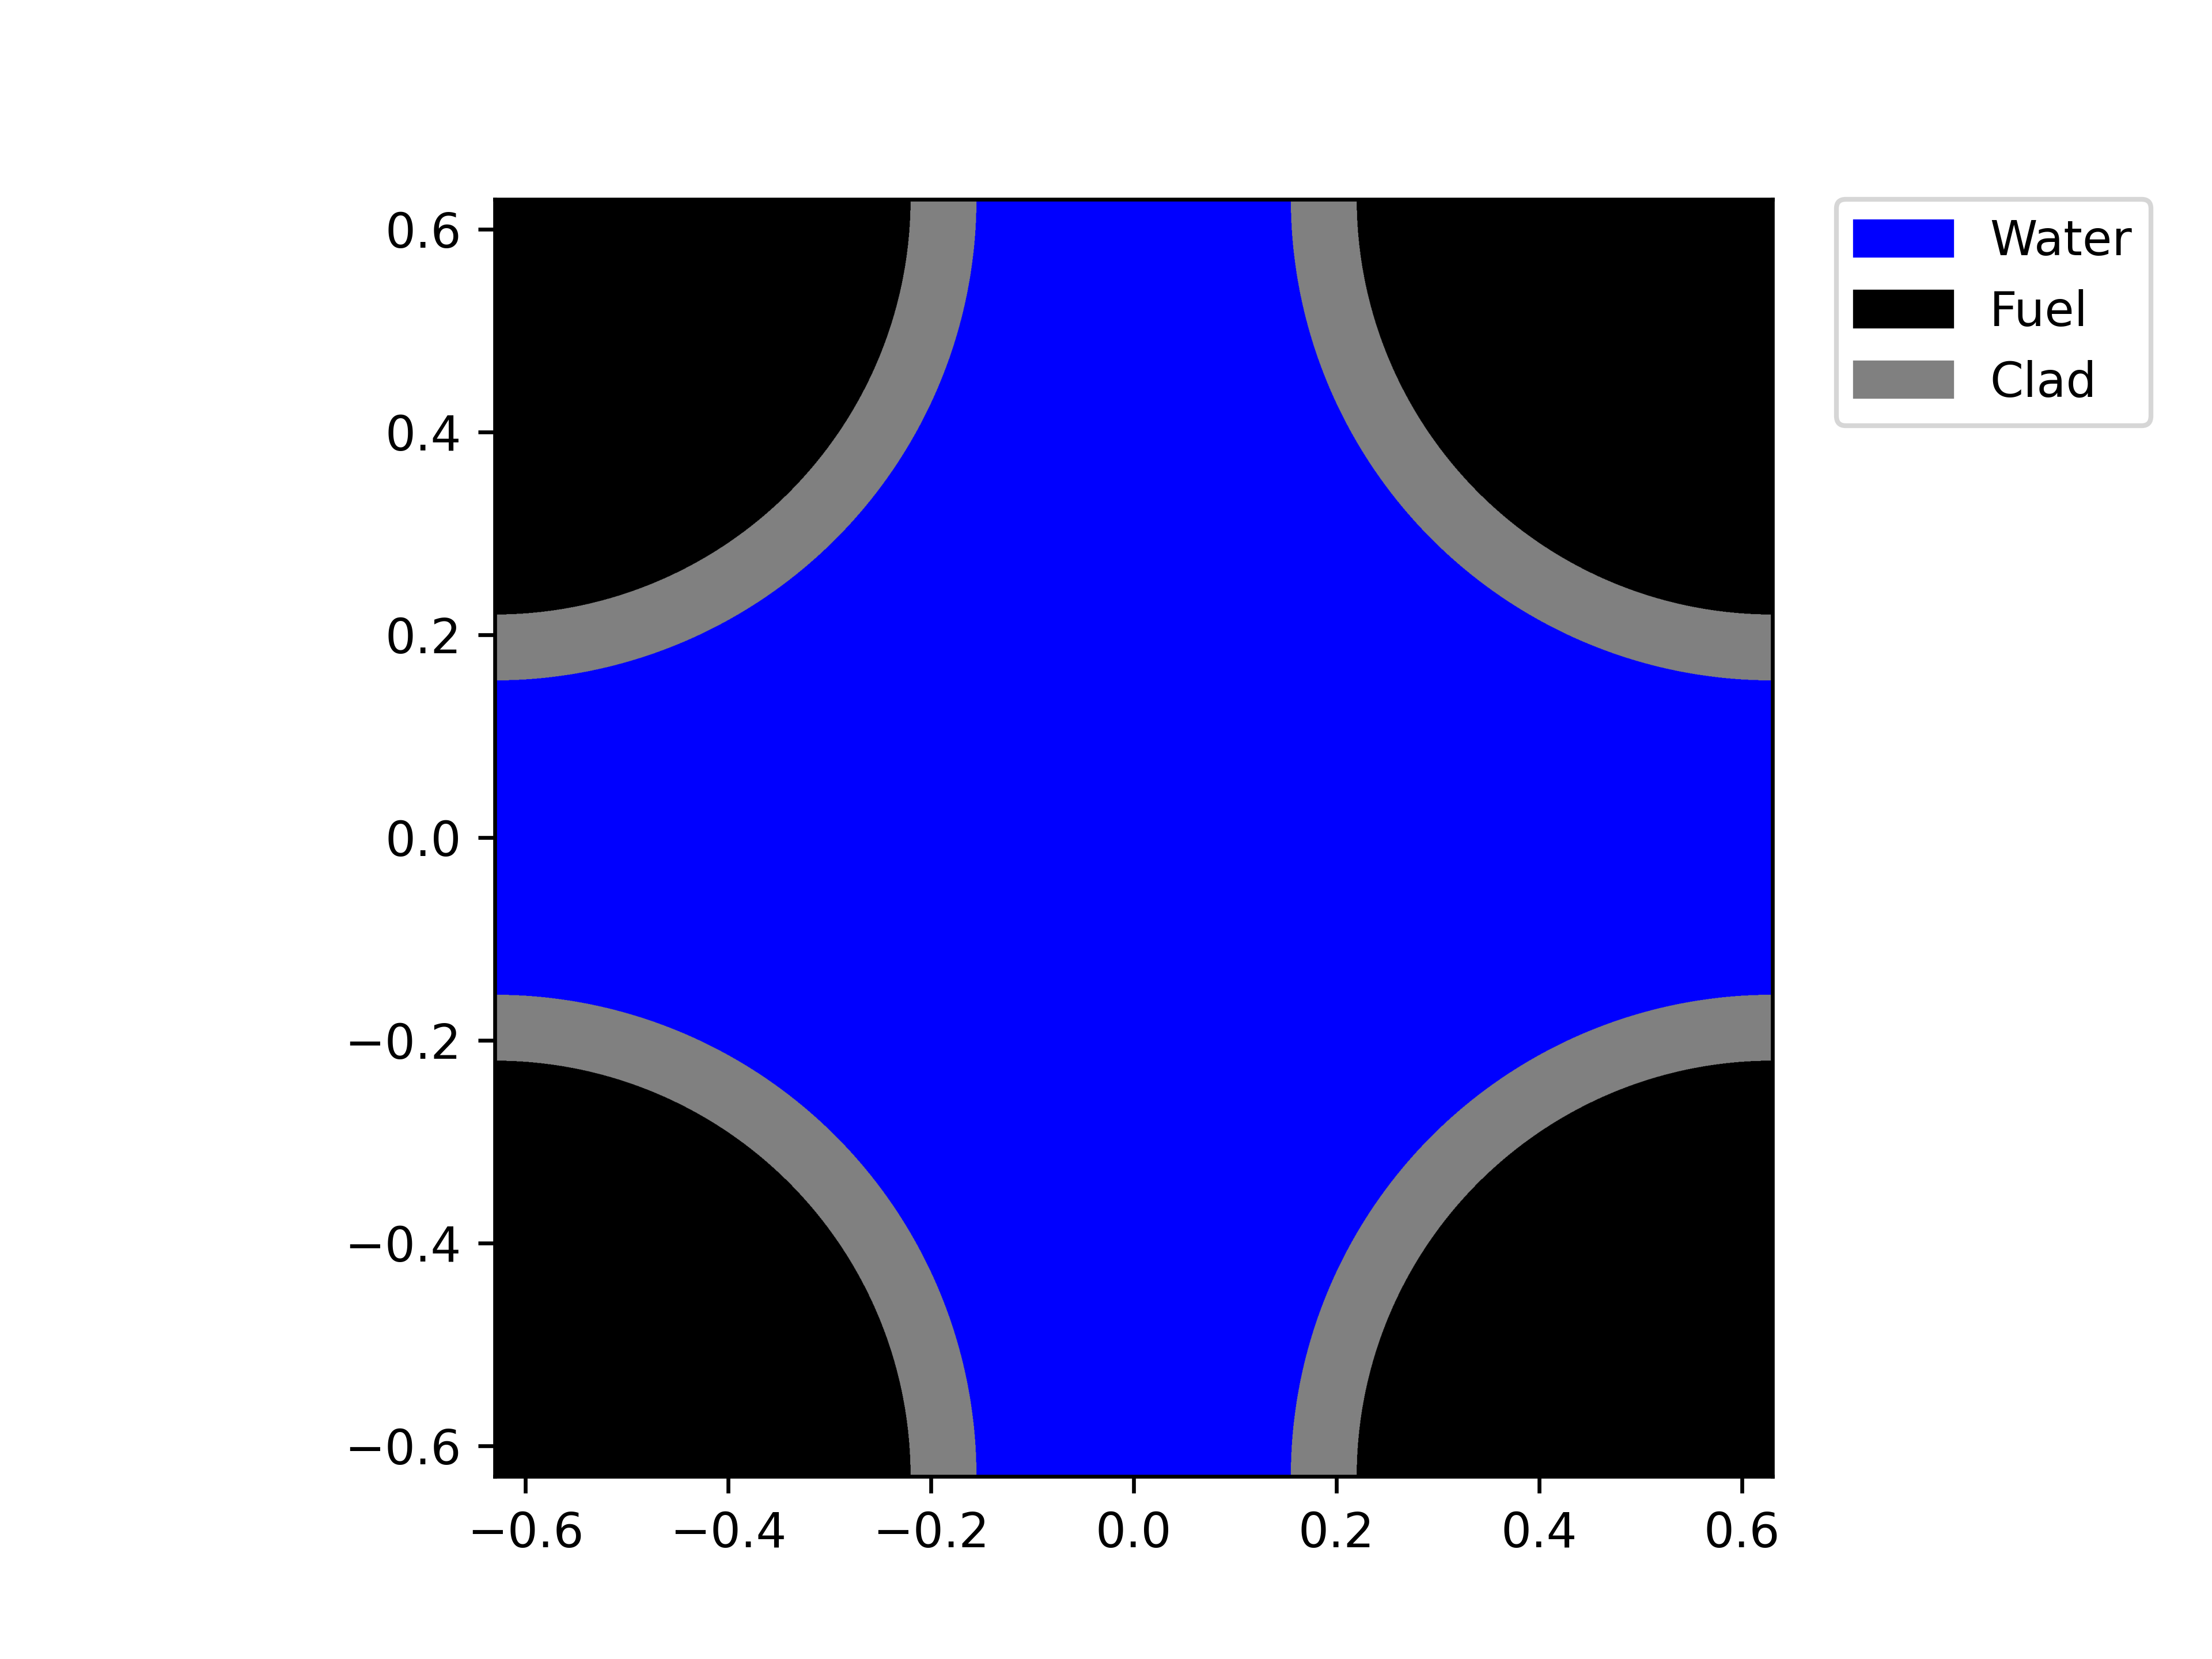
\includegraphics[width=0.5\linewidth]{geometry.png}
    \caption{Problem Geometry}
    \label{fig:geom}
\end{figure}
\clearpage
Next, we get into our initial conditions and properties for the PWR and BWR case. These are presented below, in Table \ref{tab:ICs}. All other properties are found with the use of pyXSteam, a python module interpolating steam tables.

\begin{table}[!hp!]
    \centering
    \caption{Initial Conditions and Properties}
    \label{tab:ICs}
    \renewcommand{\arraystretch}{1.5}
    \begin{tabular}{|c|c|c|c|}
         \cline{3-4}
         \multicolumn{2}{c|}{} & \textbf{PWR} & \textbf{BWR}\\
         \cline{3-4}
         \bottomrule
         \multirow{5}{*}{\textbf{Geometry}} &Channel Height (H) [$m$] & 4 & 4.1 \\
         &Pitch [$cm$]& 1.26 & 1.62 \\
         &Rod Diameter [$cm$]& 0.95& 1.227\\
         &Fuel Diameter [$cm$]& 0.82 & 1.04\\
         &Gap Thickness [$cm$]& 0.006 & 0.010 \\
         \toprule
         \bottomrule
         \multirow{3}{*}{\textbf{Thermal Conductivity}} & Gap $\bigr[\frac{W}{m^oC}\bigr]$& 0.25 & 0.25 \\
         &Fuel $\bigr[\frac{W}{m^oC}\bigr]$& 3.6 & 3.6\\
         &Clad $\bigr[\frac{W}{m^oC}\bigr]$& 21.5 & 21.5\\
         \toprule
         \bottomrule
         \multirow{4}{*}{\textbf{Conditions}}& Mass Flux $\bigr[\frac{kg}{m^2s}\bigr]$& 4000 & 2350 \\
         & Maximal Linear Power ($q'_0$) $\bigr[\frac{W}{cm}\bigr]$& 430 & 605 \\
         & Inlet Pressure [$MPa$]& 15 & 7.5 \\
         & Inlet Temperature [$^oC$]& 277 & 272 \\
         \toprule
         
    \end{tabular}
    
\end{table}

\clearpage
\section{Methods}
With our problem statement defined, and our initial conditions set, we can begin the solution process. This section will present the differential equations and equations being solved in Section \ref{modeling}, and the numerical method utilized to solve each in Section \ref{nummet}.

\subsection{Modeling}\label{modeling}
Prior to deriving the appropriate differential equations to this problem, the general differential equations are written. First, the area-averaged navier stokes equations are presented in Equations \ref{eq:massA} through \ref{eq:energyA}. Then, the general heat diffusion equation is presented in equation \ref{eq:heat}.

\begin{subequations}
    \begin{equation}
        \pd{\rho}{t}{} + \pd{\rho v}{z}{} = 0
        \label{eq:massA}
    \end{equation}
    \begin{equation}
        \pd{\rho v}{t}{} + \pd{}{z}{}\rho v^2 = -\pd{P}{z}{}-\tau_F\frac{\xi_w}{A_f} - \rho g \sin(\theta)
        \label{eq:momentumA}
    \end{equation}
    \begin{equation}
        \pd{\rho h}{t}{} + \pd{}{z}{}\rho v h = \frac{q''\xi_h}{A}+\pd{P}{t}{} + q'''
        \label{eq:energyA}
    \end{equation}
\end{subequations}

\begin{equation}
    \nabla \cdot k\nabla T + q''' = -\rho c_p \pd{T}{t}{}
    \label{eq:heat}
\end{equation}


\subsubsection{Fluid Flow}
First, the fluid flow.

First, assumption \circled{1} drops all time dependent terms from each equation. Next, assumption \circled{2} drops the heat generation term in Equation \ref{eq:energyA}. Then, defining $G = \rho v$, and then investigating the mass equation, Equation \ref{eq:massA}, G must be constant in z. Applying both of these to the momentum and energy equations yields:

\begin{subequations}
    \begin{equation}
        -\pd{P}{z}{} = G^2\pd{}{z}{}\frac{1}{\rho} +\tau_F\frac{\xi_w}{A_f} - \rho g \sin(\theta)
        \label{eq:mom2}
    \end{equation}
    \begin{equation}
        G\pd{h}{z}{} = \frac{q'' \xi_h}{A} 
        \label{eq:en2}
    \end{equation}
\end{subequations}

Now, we do not have information on $q''$, but $q'$ is known. Thus, performing a control volume analysis we can determine a relationship. All heat in/out of the pin must be equal to the heat generated, as no energy is stored:
\begin{subequations}
\begin{equation}
        q'dz = q''\xi_hdz
\end{equation}
\begin{equation}
        \frac{q'}{\xi_h} = q''
\end{equation}
\end{subequations}

And thus,

\begin{equation}
    q''(z) = \frac{q'_0}{\xi_h}\sin\bigr(\frac{\pi z}{H}\bigr)
    \label{eq:qpp}
\end{equation}
\newcommand{\qpp}{q'_0\sin\bigr(\frac{\pi z}{H}\bigr)}

Next, $h$ is not particularly helpful to solve for, thus we convert it to $\chi_e$. $\chi_e$ is a much more helpful variable, as with this we can find two phase material properties exceedingly easy, this will be touched on next. We convert $h$ to $\chi_e$ as follows:
\begin{subequations}
    \begin{equation}
        h = h_f + h_{fg}\chi_e
    \end{equation}
    \begin{equation}
        \pd{h}{z}{} = h_{fg}\pd{\chi_e}{z}{}
        \label{eq:xe2h}
    \end{equation}
\end{subequations}

Next, to apply the HEM to the momentum equation, we simply convert $\rho$ to $\rho_m$. This new $\rho_m$ is defined as:

\begin{subequations}
    \begin{equation}
        \rho_m = \bigr(V_f + V_{gf}\chi\bigr)^{-1}
    \end{equation}
    \begin{equation}
        \pd{}{z}{}\frac{1}{\rho} = V_{gf}\pd{\chi}{z}{}
    \end{equation}
    \label{eq:rhom}
\end{subequations}

Lastly, $\tau_F$ is defined as:
\begin{subequations}
\begin{equation}
    \tau_f = \frac{1}{2}f\frac{G^2}{\rho_m}
    \label{eq:tauf}
\end{equation}
\begin{equation}
    f = f_{1\Phi}\biggr(\frac{\mu_m}{\mu_f}\biggr)^n
\end{equation}
\begin{equation}
    \mu_m = \biggr( \frac{\chi}{\mu_g} + \frac{1 - \chi}{\mu_f}\biggr)^{-1}
\end{equation}
\end{subequations}


Finally, we insert Equations \ref{eq:qpp}, \ref{eq:xe2h}, \ref{eq:rhom}, and \ref{eq:tauf} into the momentum and energy equations, Equations \ref{eq:en2} and \ref{eq:mom2}, respectively. 

\begin{subequations}
    \begin{equation}
        -\pd{P}{z}{} = G^2V_{gf}\pd{\chi}{z}{} +\tau_F\frac{\xi_w}{A_f} - \rho g \sin(\theta)
    \end{equation}
    \begin{equation}
        G\biggr[\chi_e\pd{h_{fg,sat}}{z}{} + \pd{h_{f,sat}}{z}{} + h_{fg}\pd{\chi_e}{z}{} \biggr] = \frac{q'' \xi_h}{A} 
    \end{equation}
\end{subequations}

And then simplifying and rearranging, the energy equation becomes:    \begin{equation}
    \pd{\chi_e}{z}{} = \frac{1}{AGh_{fg}}q'(z) - \frac{1}{h_{fg}}\biggr[\chi_e\pd{h_{fg}}{z}{} + \pd{h_f}{z}{}\biggr]
\end{equation}

or alternatively: 
\begin{equation}
    \pd{\chi_e}{z}{} = \frac{1}{AGh_{fg}}q'(z) - \frac{1}{h_{fg}}\biggr[\chi_e\pd{h_{g}}{z}{} + (1-\chi_e)\pd{h_f}{z}{}\biggr]
    \label{eq:energy}
\end{equation}

Then, recognizing the derivative of $\rho_m$ is dependent on the derivative $\chi_e$, we substitute this derivative into $\rho_m$ and simplify. This yields:
\begin{equation}
    -\pd{P}{z}{} = 
    \frac{
    \frac{1}{2}f\frac{\xi_wG^2}{A_f\rho_m} + \rho_m g + \frac{GV_{gf}}{Ah_{fg}}\qpp
    }{1- \frac{G^2V_{gf}}{h_{fg}}\biggr[ \chi_e\pd{h_{g}}{z}{} + (1-\chi_e)\pd{h_f}{z}{}\biggr]}
    \label{eq:momentum}
\end{equation}

\subsubsection{Heat Transfer}
Next, the convective heat transfer between the fluid and the clad surface. 

In this problem set-up there are two regimes of convective heat transfer: $1\Phi$ and $2\Phi$. The criteria determining which region governs the heat transfer is the clad surface temperature. If the clad surface temperature is equal to the fluid saturation temperature or greater, then the surface is experiencing $2\Phi$ heat transfer, otherwise it is $1\Phi$. 

To begin, we investigate the first, $1\Phi$. This regime is the simple case, and its governing equation is:
\begin{equation}
    q''(z) = h\bigr[T_{s}(z) - T_{fluid}(z)\bigr]
\end{equation}

where h is found from the Dittus-Boelter correlation:

\begin{equation}
    h = \frac{Nuk}{D_h}Re^{0.8}Pr^{0.4}
\end{equation}

Next, we investigate $2\Phi$. The governing equation is the correlation:
\begin{equation}
    q'' = \sqrt{\bigr[ Fh_{fc}(T_s(z) - T_{fluid})\bigr]^2 + \bigr[ Sh_{nb}(T_s(z) - T_{sat}(z))\bigr]^2} 
    \label{2phase}
\end{equation}
Where $h_{fc}$ is the same heat transfer coefficient as in $1\Phi$, and the other parameters are defined as:

\begin{subequations}
    \begin{equation}
        F = \biggr[ 1 + \chi Pr\biggr(\frac{\rho_f}{\rho_g} - 1\biggr)\biggr] ^{-1}
    \end{equation}  
    \begin{equation}
        S = \bigr[1 + 0.055F^{0.1}Re^{0.16}\bigr]^{-1}
    \end{equation}
    \begin{equation}
        h_{nb} = 55 \biggr(\frac{P}{P_c}\biggr)^{0.12}(q'')^{2/3}\biggr(-\log\frac{P}{P_c}\biggr)M_{H_2O}^{-1/2}
        \label{eq:hnb}
    \end{equation}
\end{subequations}

Next, we investigate the CHF criteria for both PWRs and BWRs. PWRs undergo low-quality CHF, also known as Departure from Nucleate Boiling (DNB). BWRs can also undergo this, but are more likely to experience high-quality CHF, also known as dryout. Dryout occurs at some critical power, and thus the thermal design for BWRs is Critical Power Ratio (CPR). Similarly, DNB occurs at some power, and thus the thermal design criteria for PWRs is DNB Ratio (DNBR). 

Firtly, DNBR. DNBR is defined as:
\begin{equation}
    DNBR = \frac{q''_{critical}}{q''_{operating}}
\end{equation}
where $q''_{critical}$ is the subject of numerous correlations. The one utilized in this work is the W-3 correlation \cite{tong}. This correlation is:
\begin{subequations}
    \label{eq:dnbr}
    \begin{equation}
        q''_cr = c_1c_2c_3c_4c_5
    \end{equation}
    \begin{equation}
        c_1 = (2.022 - 0.06238P) + (0.1722 - 0.01427P)\exp[(18.177-0.5987P)\chi_e]
    \end{equation}
    \begin{equation}
        c_2 = (0.1484 - 1.596\chi_e + 0.1729\chi_e|\chi_e|)\cdot 2.326G + 3271
    \end{equation}
    \begin{equation}
        c_3 = 1.157 - 0.869\chi_e
    \end{equation}
    \begin{equation}
        c_4 = 0.2664 + 0.8357\exp[-124.1D_h]
    \end{equation}
    \begin{equation}
        c_5 = 0.8258 + 0.000341(h_f - h_{in})
    \end{equation}
\end{subequations}

Next, CPR. CPR is defined as the power scaling factor that causes the steam quality to be tangent to the the critical steam quality. The scaling factor is found iteratively, but the critical steam quality is found utilizing the CISE-4 \cite{tk} correlation:

\begin{subequations}
    \label{eq:critx}
    \begin{equation}
        \chi_{cr} = \biggr(a\frac{L_{cr}}{L_cr + b}\biggr)
    \end{equation}
    \begin{equation}
        a = \frac{1 - \frac{P}{P_c}}{(G/1000)^{1/3}}
    \end{equation}
    \begin{equation}
        b = 0.199\biggr(\frac{P_c}{P} - 1\biggr)^{0.4}GD^{1.4}
    \end{equation}
\end{subequations}



\subsubsection{Fuel Pin}
Finally, we derive the temperature distribution in the fuel pin. This pin has three regions: Fuel ($_f$), Gap ($_g$), and Clad ($_c$). Applying Assumptions \circled{1}, \circled{3}, and \circled{6}, we obtain the following simplified heat diffusion equations for each region:
\newcommand{\laplace}{\frac{1}{r}\pd{}{r}{}r\pd{}{r}{}}
\begin{subequations}
\begin{equation}
    k_f\laplace T_f(r,z) + q''' = 0
\end{equation}
\begin{equation}
    k_g\laplace T_g(r,z) = 0
\end{equation}
\begin{equation}
    k_c\laplace T_c(r,z) = 0
\end{equation}
\end{subequations}

First, solving the fuel temperature distribution:
\begin{subequations}
    \begin{equation}
        k_f\laplace T_f(r,z) + q'''(z) = 0
    \end{equation}
    \begin{equation}
        \laplace T_f(r,z) = -\frac{q'''(z)}{k_f}
    \end{equation}
    \begin{equation}
        r\pd{}{r}{}T_f(r,z) = -\frac{q'''(z)r^2}{2k_f} + C_1(z)
    \end{equation}
    \begin{equation}
        T_f(r,z) = -\frac{q'''(z)r^2}{4k_f} + C_1(z)\ln(r) + C_2(z)
        \label{eq:fgen}
    \end{equation}
\end{subequations}

Then for the gap:
\begin{subequations}
    \begin{equation}
        k_g\laplace T_g(r,z) = 0
    \end{equation}
    \begin{equation}
        r\pd{}{r}{}T_g(r,z) = C_3(z)
    \end{equation}
    \begin{equation}
        T_g(r,z) = C_3(z)\ln(r) + C_4(z)
        \label{eq:ggen}
    \end{equation}
\end{subequations}

and finally, for the clad:
\begin{subequations}
    \begin{equation}
        k_c\laplace T_c(r,z) = 0
    \end{equation}
    \begin{equation}
        r\pd{}{r}{}T_c(r,z) = C_5(z)
    \end{equation}
    \begin{equation}
        T_c(r,z) = C_5(z)\ln(r) + C_6(z)
        \label{eq:cgen}
    \end{equation}
\end{subequations}

\clearpage
Next, for our boundary conditions. The boundary conditions for this problem are:

\begin{itemize}
    \item[\circled{1}] $-k_f\nabla T_f (r = 0,z) = 0$
    \item[\circled{2}] $-k_f\nabla T_f(r=R_{f},z) = -k_g\nabla T_g(r=R_{f},z)$
    \item[\circled{3}] $-k_g\nabla T_g(r=R_{c,i},z)=-k_c\nabla T_c(r=R_{c,i},z)$
    \item[\circled{4}] $T_c(r= R_{c,s},z) = T_{c,s}(z)$
    \item[\circled{5}] $T_g(r=R_{c,i},z) = T_c(r=R_{c,i},z)$
    \item[\circled{6}] $T_f(r=R_f,z) = T_g(r=R_f,z)$
\end{itemize}

In applying all boundary conditions, once an unknown (such as $C_1$) is found, it will be kept as it initially appears and not expanded out for brevity. First, applying \circled{1} eliminates $C_1$, as the natural logarithm of 0 is non-finite, and thus the derivative cannot be 0. Next, investigating \circled{2}, inserting temperature distributions into this relation yields:

\begin{subequations}
    \begin{equation}
        \frac{q'''(z)R_f}{2} = -\frac{k_gC_3}{R_f}
    \end{equation}
    \begin{equation}
        C_3(z) = -\frac{q'''(z)R_f^2}{2k_g}
    \end{equation}
\end{subequations}

Then, applying \circled{3}, and inserting the corresponding temperature distributions:

\begin{subequations}
    \begin{equation}
        -\frac{k_gC_3(z)}{R_{c,i}} = -\frac{k_cC_5(z)}{R_{c,i}}
    \end{equation}
    \begin{equation}
        C_5(z) = \frac{k_g}{k_c}C_3(z)
    \end{equation}
\end{subequations}

Then, applying \circled{4}, assuming $T_{c,s}$ is a known value, found through convective heat transfer analysis at the boundary:
\begin{subequations}
    \begin{equation}
        C_5(z)\ln(R_{c,s}) + C_6(z) = T_{c,s}(z)
    \end{equation}
    \begin{equation}
        C_6(z) = T_{c,s}(z) - C_5(z)\ln(R_{c,s})
    \end{equation}
\end{subequations}

Proximally applying \circled{5}:

\begin{subequations}
    \begin{equation}
        C_3(z)\ln(R_{c,i}) + C_4(z) =  C_5(z)\ln(R_{c,i}) + C_6(z)
    \end{equation}
    \begin{equation}
        C_4(z) = \ln(R_{c,i})\bigr[C_5(z) - C_3(z)\bigr] + C_6(z)
    \end{equation}
\end{subequations}

And finally, applying the final boundary condition, \circled{6}:
\begin{subequations}
    \begin{equation}
        -\frac{q'''(z)R_{f}^2}{4k_f} + C_2(z) = C_3(z)\ln(R_f) + C_4(z)
    \end{equation}
    \begin{equation}
         C_2(z) = \frac{q'''(z)R_{f}^2}{4k_f} + C_3(z)\ln(R_f) + C_4(z)
    \end{equation}
\end{subequations}

\subsection{Numerical Methods}\label{nummet}
The numerical method utilized in solving this problem is known as 'forward' finite differencing. This scheme is utilized because the 'next' point in the simulation is only dependent on the previous' results. A simple example of this is in approximating the first derivative of a function. Forward finite differencing is defined such that the approximation to the first derivative is in the form of 'rise over run', like so:

\begin{equation}
    \pd{f(x)}{x}{} = \frac{f(x_{i+1}) - f(x_i)}{x_{i+1} - x_i}
\end{equation}

such that $i$ denotes the current node, and $i+1$ denotes the next node visited in the scheme.

In this problem, the energy equation is approximated as follows:
\begin{subequations}
    \begin{equation}
        \pd{\chi_e}{z}{} = \frac{\chi_e(z_{i+1}) - \chi_e(z_i)}{z_{i+1} - z_i}
    \end{equation}
    \begin{equation}
        \chi_e(z_{i+1}) = \chi_e(z_{i}) + \Delta z\biggr(\frac{1}{AGh_{fg}}q'(z) - \frac{1}{h_{fg}}\biggr[\chi_e(z_i)\pd{h_{g}}{z}{} + (1-\chi_e(z_i)\pd{h_f}{z}{}\biggr]\biggr)
    \label{eq:energyDis}
    \end{equation}
\end{subequations}

And then the momentum equation:

\begin{subequations}
    \begin{equation}
        -\pd{P}{z}{} = -\frac{P(z_{i+1}) - P(z_{i})}{z_{i+1} - z_i}
    \end{equation}
    \begin{equation}
        P(z_{i+1}) = P(z_i) - \Delta z\left[ 
        \frac{
        \frac{1}{2}f\frac{\xi_wG^2}{A_f\rho_m} + \rho_m g + \frac{GV_{gf}}{Ah_{fg}}\qpp
         }{1- \frac{G^2V_{gf}}{h_{fg}}\biggr[ \chi_e(z_i)\pd{h_{g}}{z}{} + (1-\chi_e(z_i))\pd{h_f}{z}{}\biggr]}
        \right]
    \end{equation}
\end{subequations}

Next, to determine the clad surface temperature, we utilize convective heat transfer. To do so, we assume at point $z_i$, the heat transfer is $1\Phi$. We then determine the wall temperature assuming this is the case, then check this found value against the saturation temperature of the water. If the $1\Phi$ wall temperature is less than the saturated wall temperature, then this value is stored as the wall temperature at that node, and the simulation progresses to the next node. On the other hand, if this assumed $1\Phi$ value is greater than the saturation temperature, then this node is experiencing $2\Phi$ heat transfer, and thus the $1\Phi$ value is incorrect. To determine the correct wall temperature with $2\Phi$ heat transfer, Equations \ref{2phase} through \ref{eq:hnb} are used. This equation yields a quadratic, and thus the wall temperature can be found one of two ways --- analytically or numerically. I elected to solve for the wall temperature numerically, leveraging \texttt{scipy.optimize.root} to determine the roots of the quadratic.

With the clad surface temperature found, the fuel pin temperature distribution is found simply through plugging in the clad surface temperature to each coefficient that is dependent on it.

Finally, to find the CPR, an iterative scheme is used. This scheme begins by finding the steam quality as a function of boiling length for the operating linear power, comparing this against the critical quality found from Equation \ref{eq:critx}. Then, the linear power is scaled by a factor $n$,  and this process is repeated. This is done until the steam quality meets the critical quality, specifically when the critical quality is tangential to the steam quality.

\clearpage
\section{Results and Analysis}
\subsection{Pressurized Water Reactor}
\subsubsection{Results}
Prior to presenting relevant results, a mesh refinement study is done to determine an appropriate mesh size. Notably, as the number of nodes used in the spatial discretization increases the difference between each solution decreases. For the remainder of the results presented, 100 nodes are utilized.

\begin{figure}[!hp!]
    \centering
    
\includegraphics[width=0.5\linewidth]{PWRplots/mesh.png}
    \caption{Mesh convergence of the coolant temperature for the PWR}
    \label{fig:pwrmesh}
\end{figure}

With an appropriate mesh size selected, we know move onto the temperature distributions. Firstly, the fluid saturation temperature as a function of axial position along the channel is presented in Figure \ref{fig:pwrcoolant}. Next, the inner and outer clad surface temperatures as a function of axial position is presented in \ref{fig:pwrclad}. Finally, the fuel outer surface and center-line temperature as a function of axial position is presented in \ref{fig:pwrfuel}. To continue, the radial temperature profile of the pin at three axial locations are found. The axial locations are at $\frac{H}{4}$, $\frac{H}{2}$, and $z_{max,cl}$, where $z_{max,cl}$ is defined as the location in which the center-line temperature is maximum. These results are presented in Figures \ref{fig:pwrh4}, \ref{fig:pwrh2}, and \ref{fig:pwrzmax}, respectively, and the maximum center-line temperature occurred at 2.01 meters along the channel. Next, the pressure as a function of axial location is presented in Figure \ref{fig:pwrpressure}. Finally, the critical heat flux, found using Equation \ref{eq:dnbr}, is presented in comparison to the operational heat flux, both as functions of axial position, in Figure \ref{fig:pwrdnb}, and the resulting ratio is presented in Figure \ref{fig:pwrdnbr}. The minimum DNBR is found to be 2.3973, well over the threshold of 1.3. 


\begin{figure}[!hp!]
    \begin{minipage}[b]{.45\linewidth}
    \centering
        
\includegraphics[width=\linewidth]{PWRplots/tfluid.png}
        \caption{PWR coolant temperature as a function of axial location}
        \label{fig:pwrcoolant}
        \vspace{4ex}
    \end{minipage}
    \begin{minipage}[b]{.45\linewidth}
    \centering
        
\includegraphics[width=\linewidth]{PWRplots/tclad.png}
        \caption{PWR clad temperature as a function of axial location}
        \label{fig:pwrclad}
        \vspace{4ex}
    \end{minipage}
    \begin{minipage}[b]{.45\linewidth}
    \centering
        
\includegraphics[width=\linewidth]{PWRplots/tfuel.png}
        \caption{PWR fuel temperature as a function of axial location}
        \label{fig:pwrfuel}
        \vspace{4ex}
    \end{minipage}
    \begin{minipage}[b]{.45\linewidth}
    \centering
        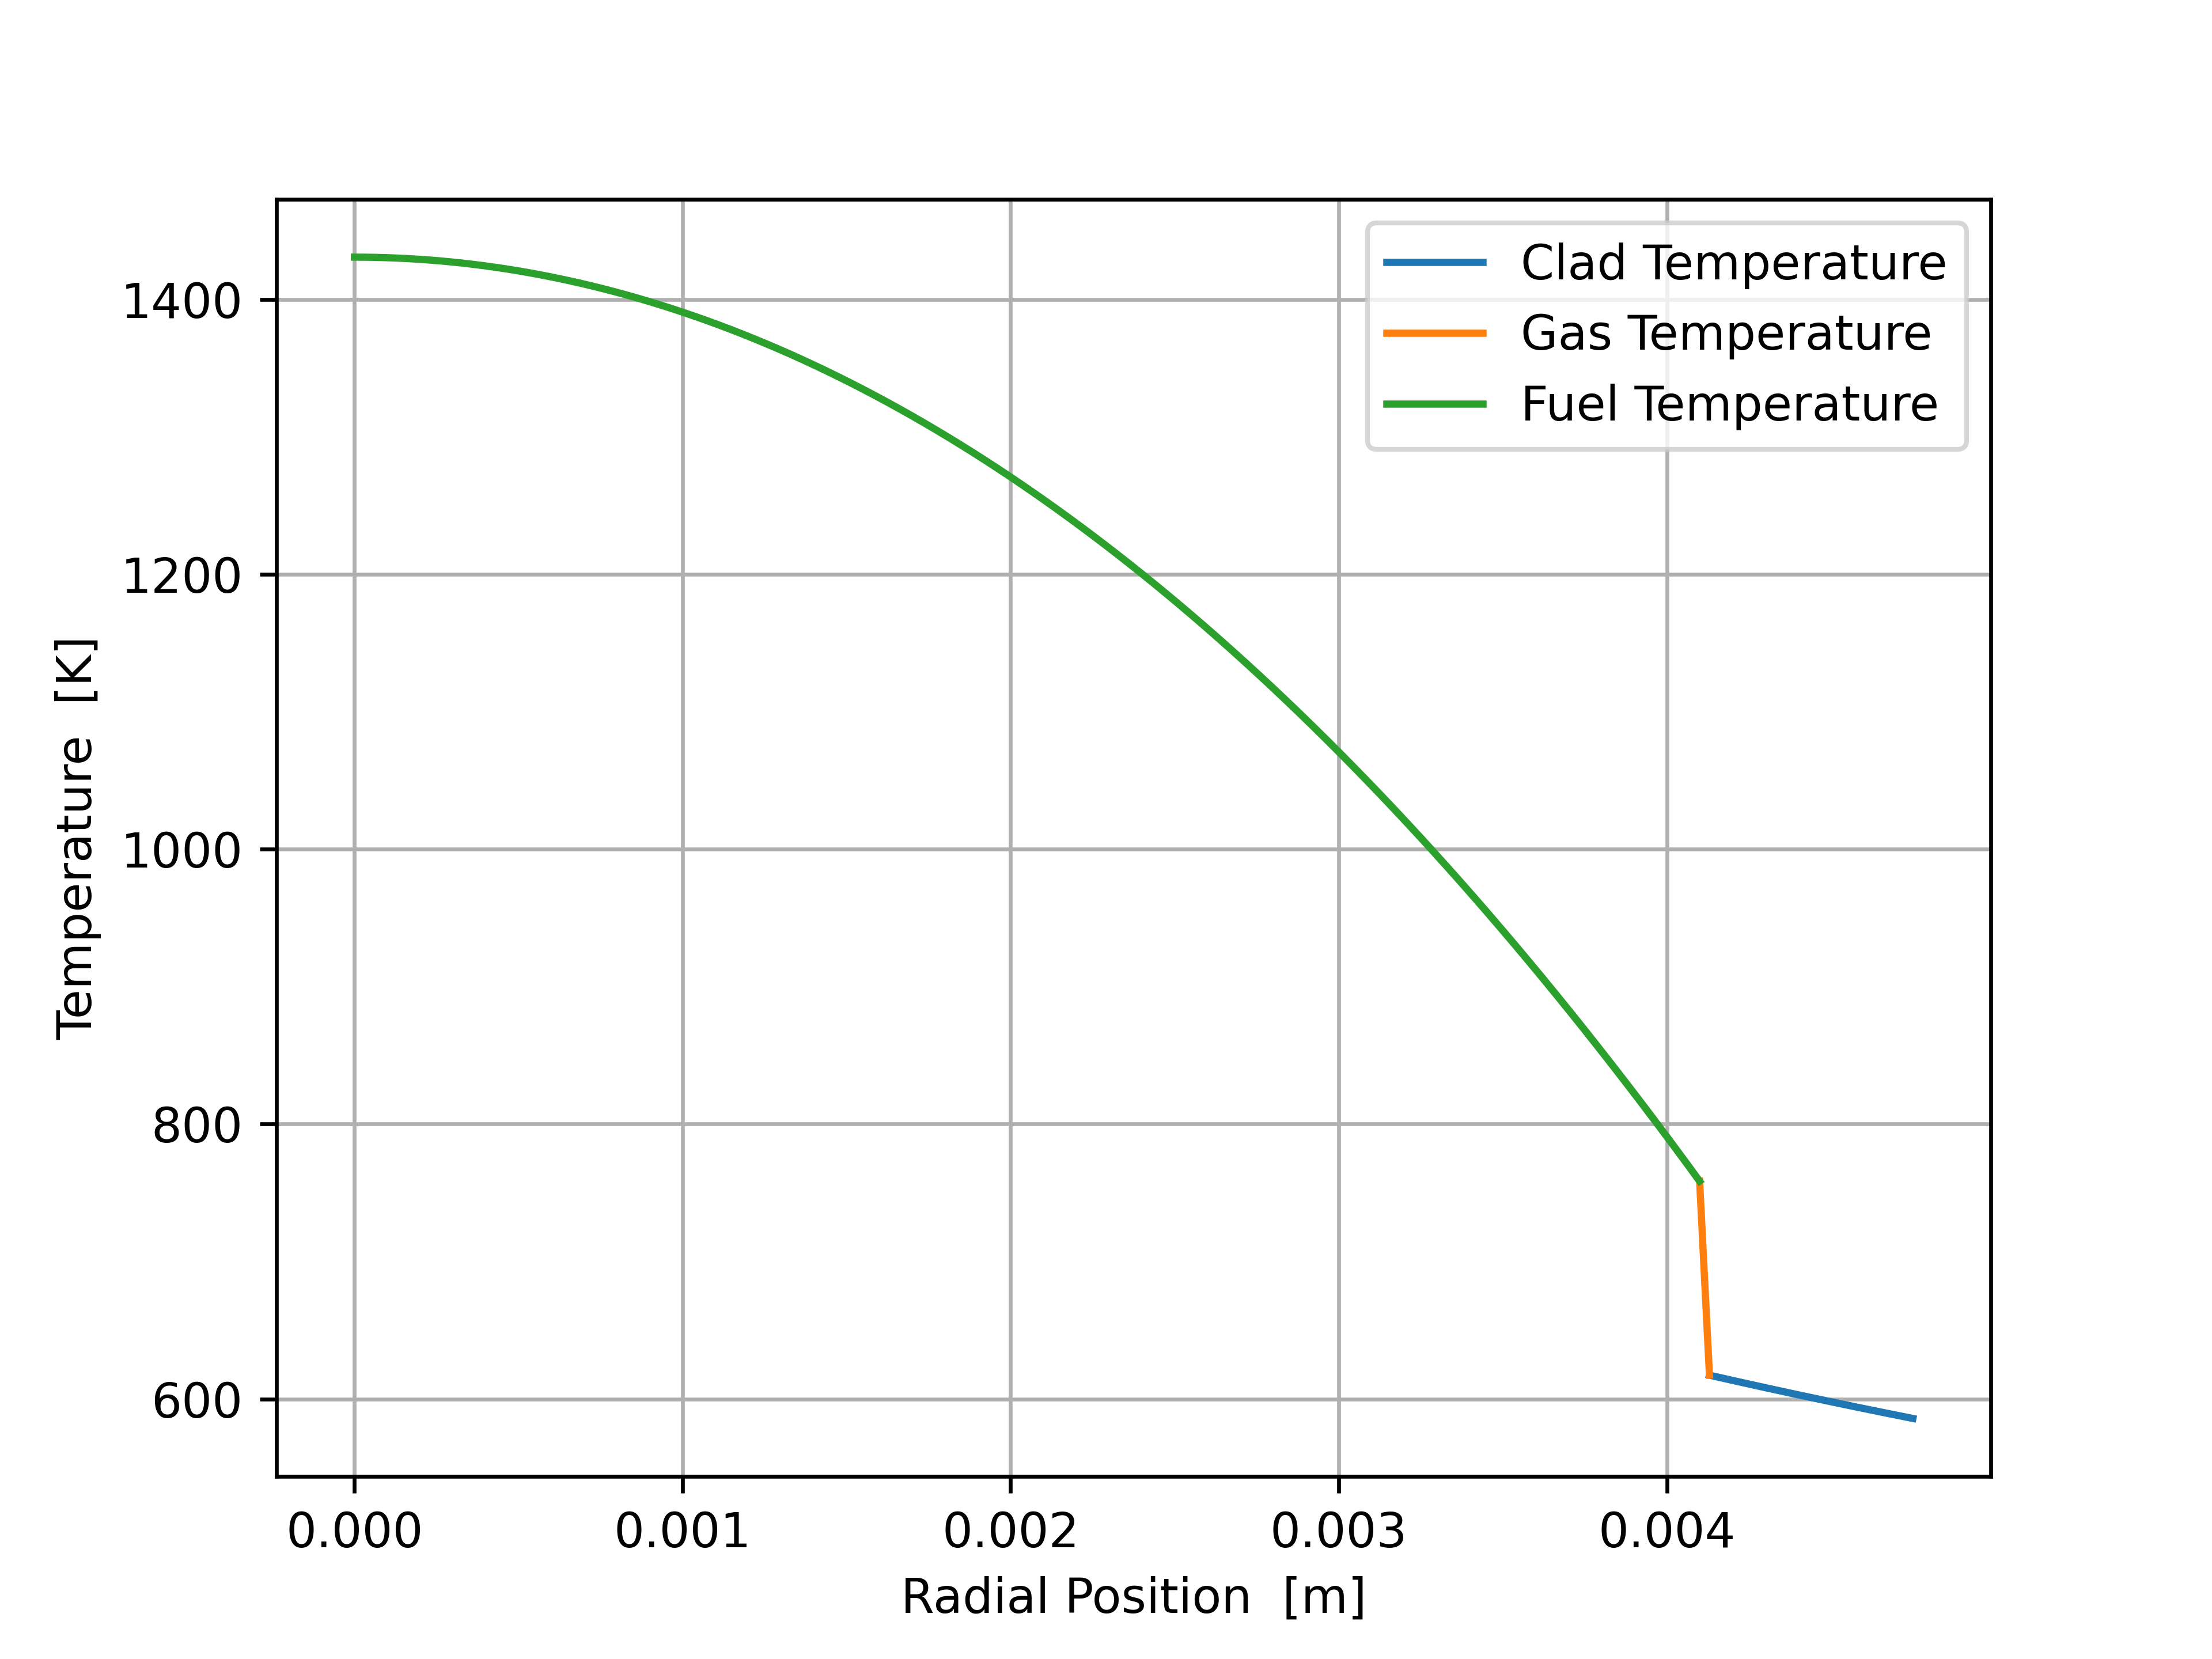
\includegraphics[width=\linewidth]{PWRplots/r-at-1.0.png}
        \caption{Radial PWR pin temperature distribution at H = 1.0 m}
        \label{fig:pwrh4}
        \vspace{4ex}
    \end{minipage}
    \begin{minipage}[b]{.45\linewidth}
    \centering
        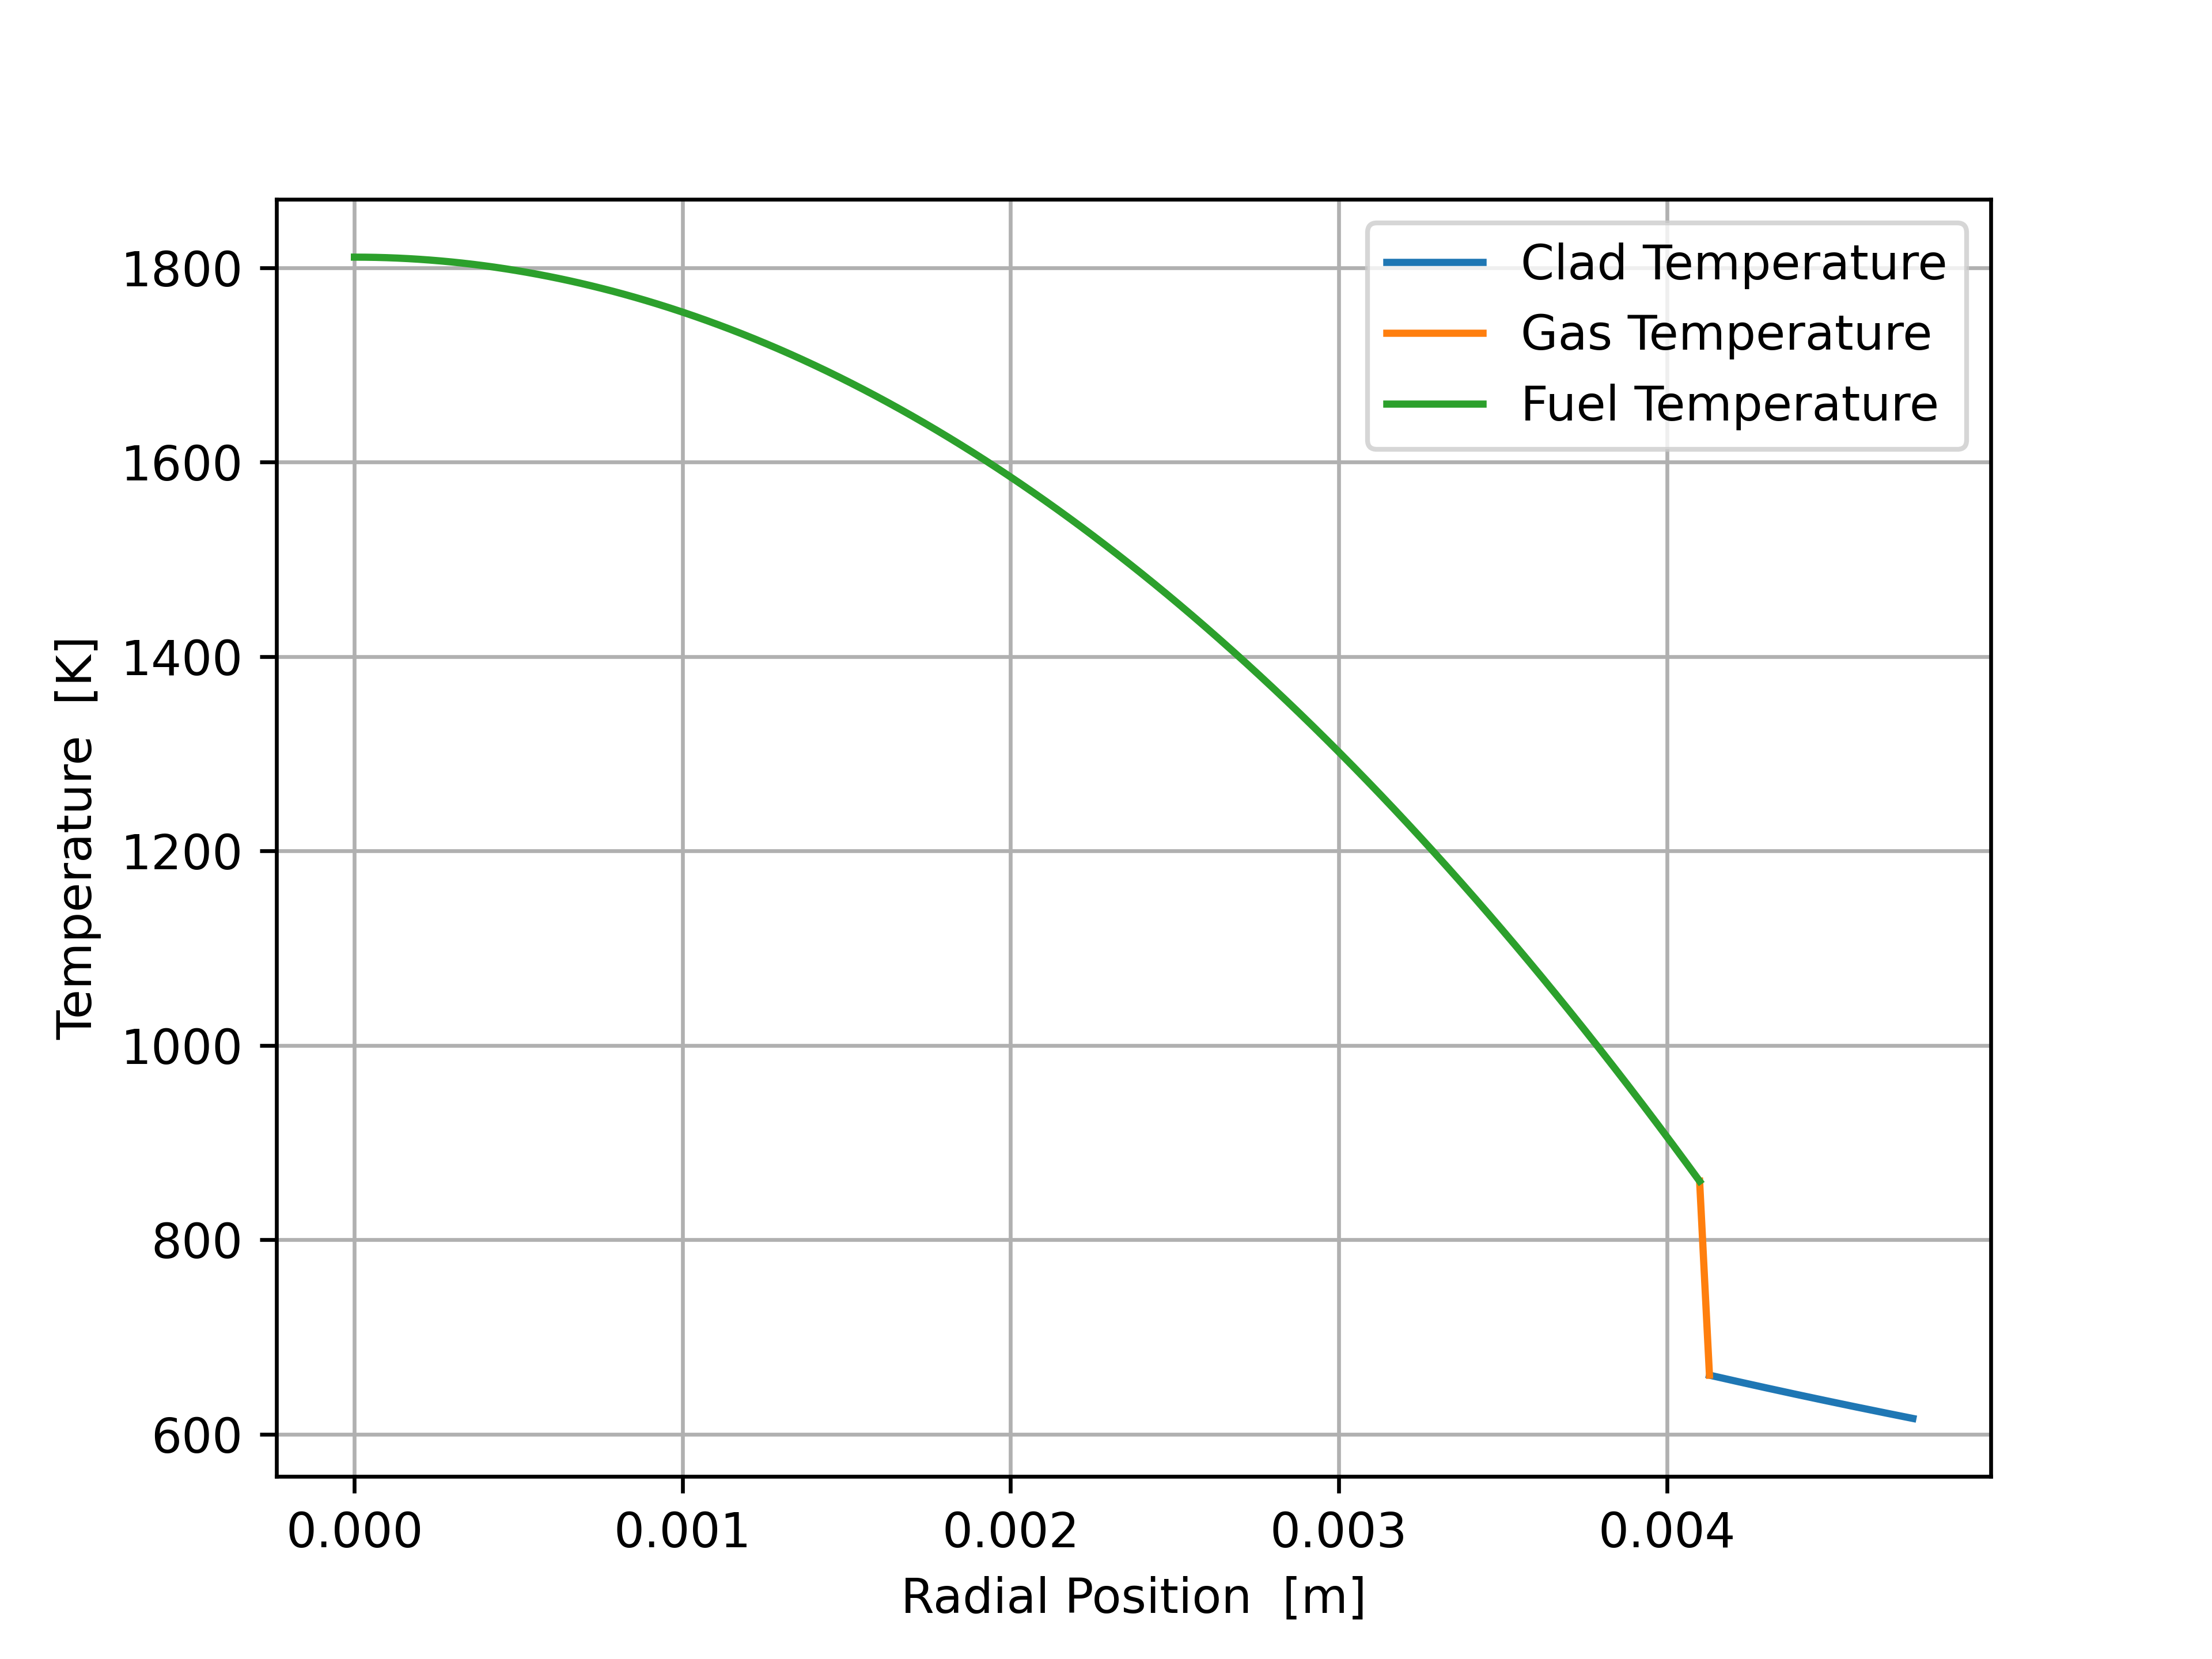
\includegraphics[width=\linewidth]{PWRplots/r-at-2.0.png}
        \caption{Radial PWR pin temperature distribution at H = 2.0 m}
        \label{fig:pwrh2}
        \vspace{4ex}
    \end{minipage}
    \begin{minipage}[b]{.45\linewidth}
    \centering
        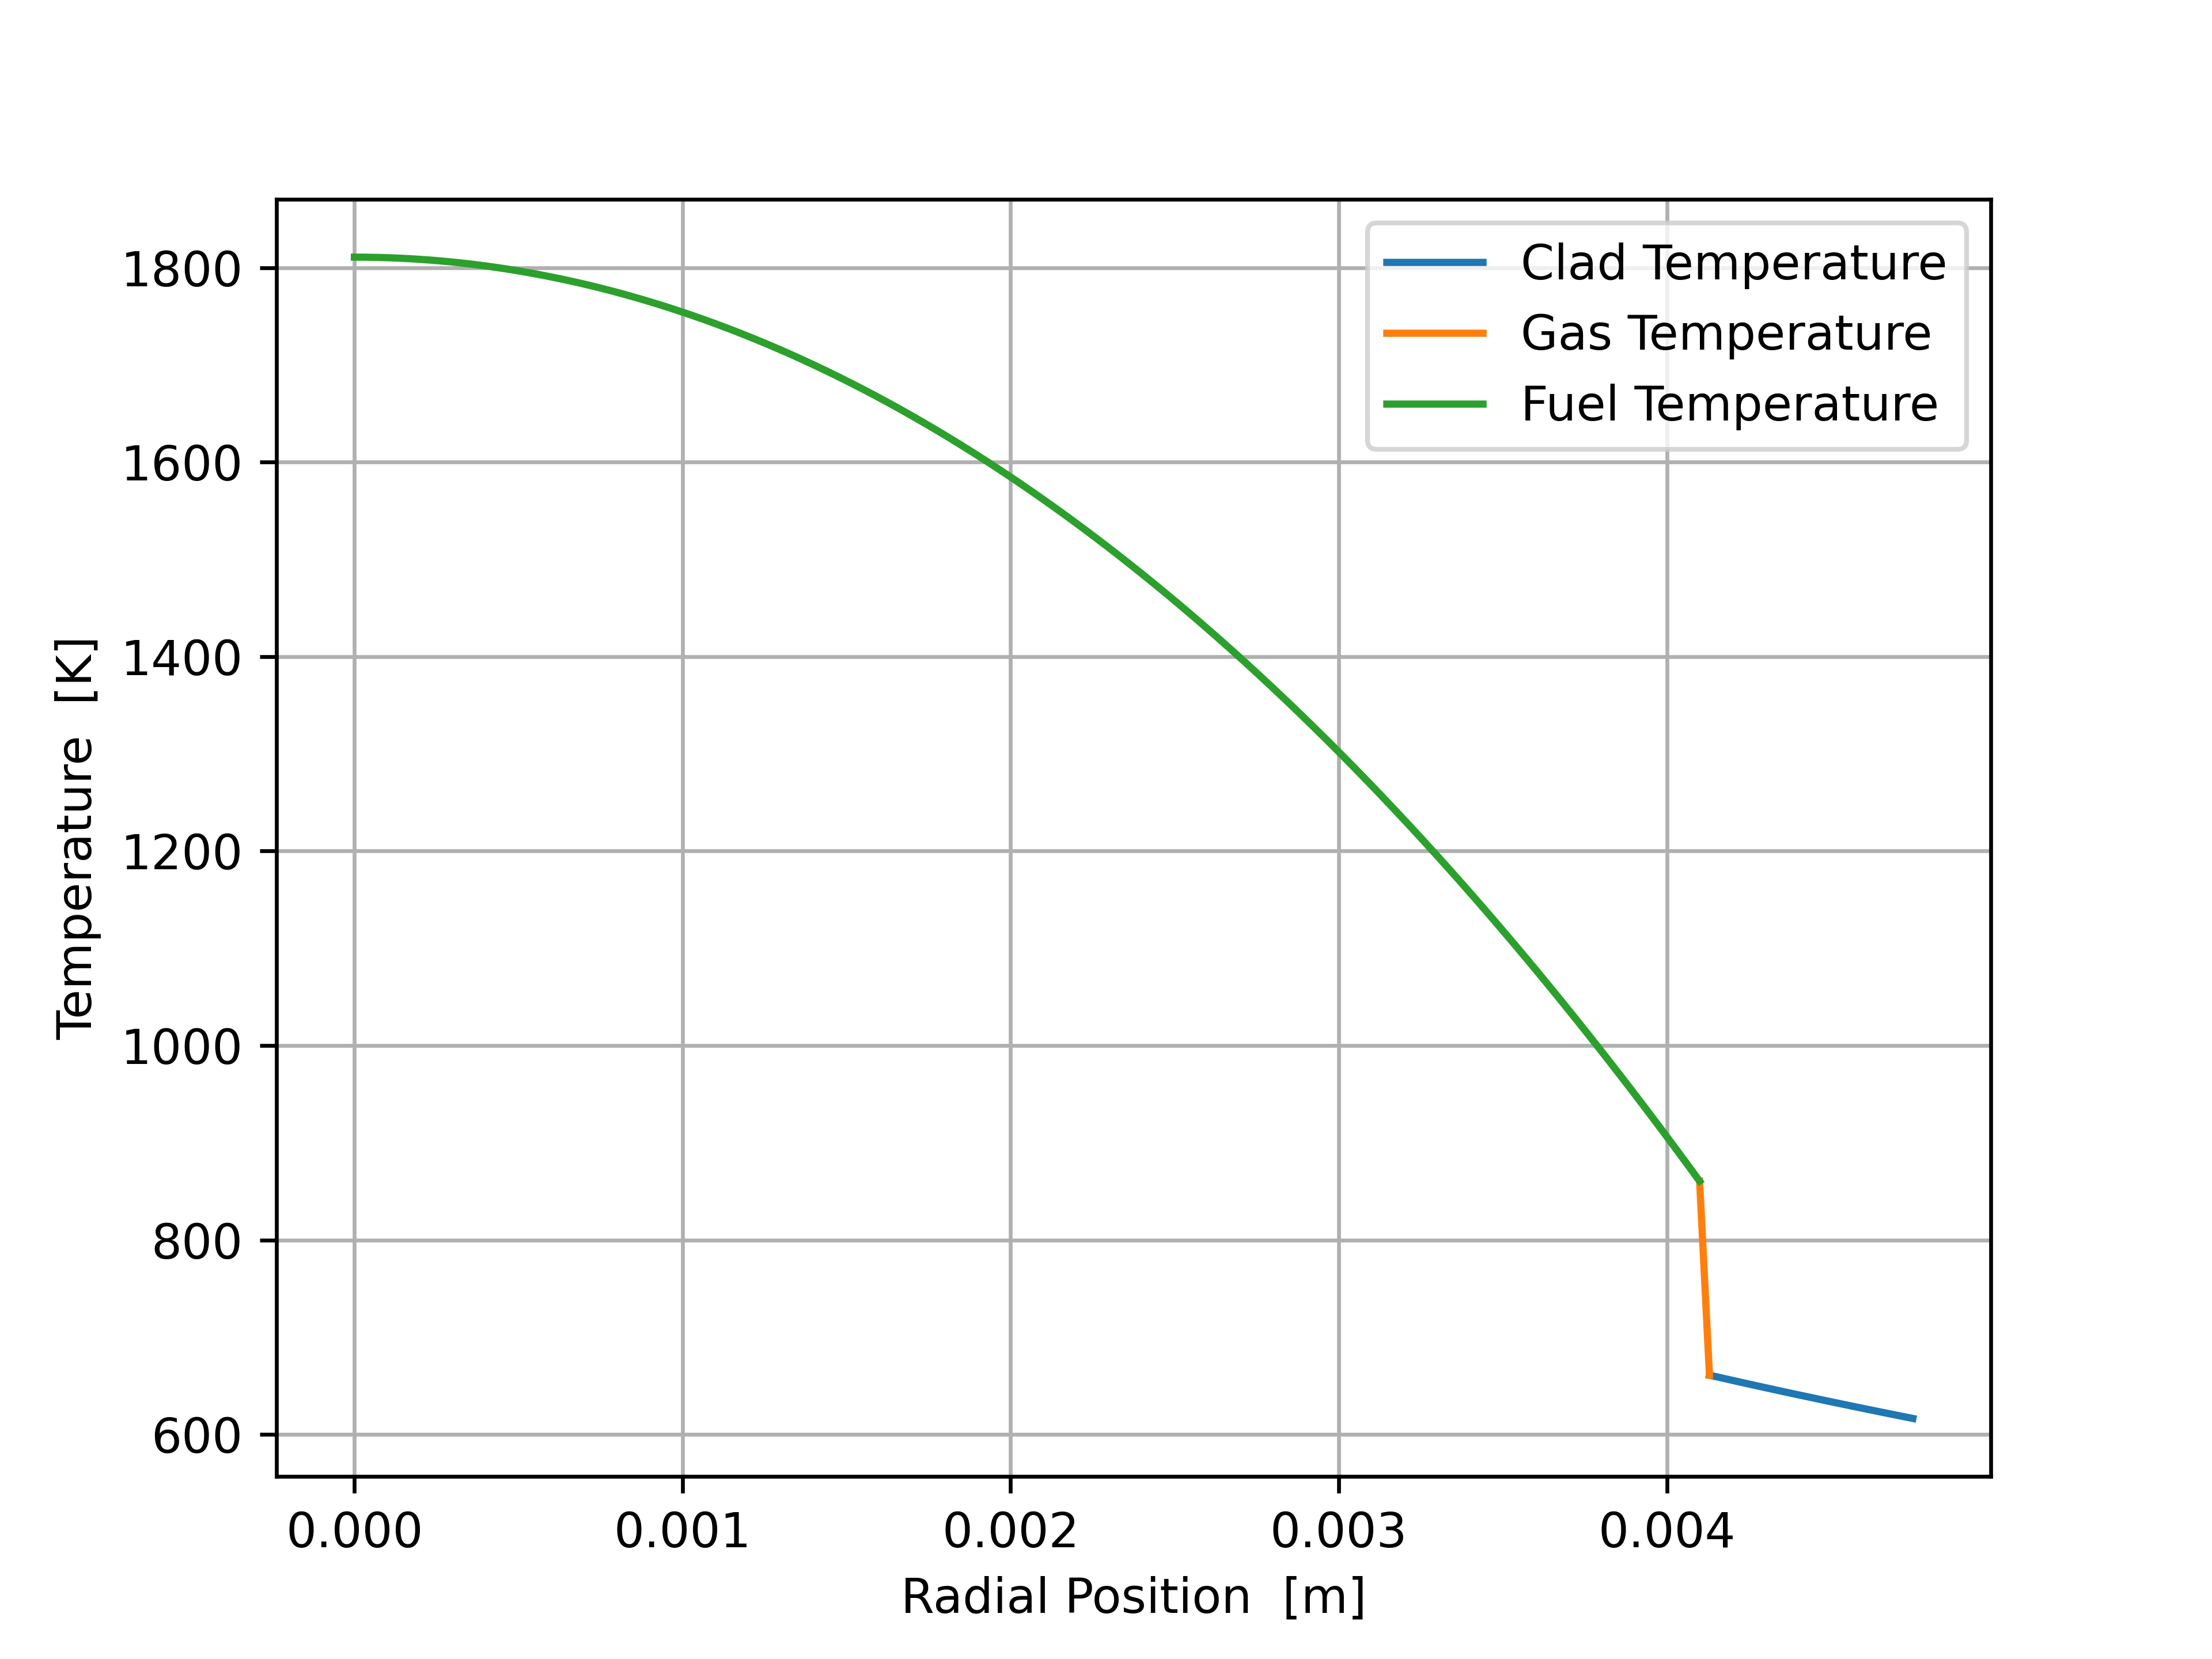
\includegraphics[width=\linewidth]{PWRplots/r-at-2.006006006006006.png}
        \caption{Radial PWR pin temperature distribution at H = 2.01 m}
        \label{fig:pwrzmax}
        \vspace{4ex}
    \end{minipage}
\end{figure}

\begin{figure}[!hp!]
    \centering
    
\includegraphics[width=0.5\linewidth]{PWRplots/pressure.png}
    \caption{PWR pressure as a function of axial location}
    \label{fig:pwrpressure}
\end{figure}

\begin{figure}[!hp!]
    \begin{minipage}[b]{.45\linewidth}
    \centering
        
\includegraphics[width=\linewidth]{PWRplots/dnb.png}
        \caption{PWR critical and operational heat flux as functions of axial location}
        \label{fig:pwrdnb}
        \vspace{4ex}
    \end{minipage}
    \begin{minipage}[b]{.45\linewidth}
    \centering
        
\includegraphics[width=\linewidth]{PWRplots/dnbr.png}
        \caption{PWR DNBR as a function of axial location}
        \label{fig:pwrdnbr}
        \vspace{4ex}
    \end{minipage}
\end{figure}

Finally, the sensitivity of the maximum center-line temperature to the maximum linear power, the mass flux, the inlet fluid temperature, and the inlet fluid pressure was investigated. To do this, simulations were re-run with 5 different values for each parameter, outputting only the maximum center-line temperature. These results are presented in Table \ref{tab:pwrsens}.

\begin{table}[!hp!]
    \centering
    \renewcommand{\arraystretch}{1.5}
    \caption{Sensitivity of PWR maximum center-line temperature to select inputs}
    \label{tab:pwrsens}
    \begin{tabular}{|c|c|c|c|c|c|c|}
        \toprule
        \bottomrule
        $q'_{0}$  [$W\cdot cm^{-1}$] & 215.0 & 322.5 & 430.0 & 537.5 & 645.0 \\
        \hline
        $T_{max,CL}$  [$K$] & 1182.065 & 1498.145 & 1811.012 & 2111.856 & 2411.461 \\
        \toprule
        \bottomrule
        $G$  [$kg\cdot m^{-2} \cdot s^{-1}$] & 2000.0 & 3000.0 & 4000.0 & 5000.0 & 6000.0 \\
        \hline
        $T_{max,CL}$  [$K$] & 1814.255 & 1813.359 & 1811.012 & 1801.556 & 1792.889 \\
        \toprule
        \bottomrule
        $T_{fluid,inlet}$  [$K$] & 492.246 & 523.012 & 553.777 & 584.542 & 609.155 \\
        \hline
        $T_{max,CL}$  [$K$] & 1762.829 & 1790.371 & 1811.646 & 1813.957 & 1814.247 \\
        \toprule
        \bottomrule
        $P_{inlet}$  [$MPa$] & 11.25 & 13.125 & 15.0 & 16.875 & 18.75 \\
        \hline
        $T_{max,CL}$  [$K$] & 1792.731 & 1802.641 & 1811.012 & 1814.371 & 1814.3 \\
        \toprule
    \end{tabular}
\end{table}

\clearpage
\subsubsection{Analysis}
To begin, investigating Figure \ref{fig:pwrcoolant}, the fluid temperature does not quite reach the saturation temperature, and peaks at 612$^o$ Kelvin. This is to be expected, as there is no bulk boiling in a PWR. Next, investigating the clad temperature distribution, we notice some odd behavior occurring after the onset of nucleate boiling. This rapid de-acceleration of the temperature increase is due to much better heat transfer, as $2\Phi$ heat transfer is orders of magnitude stronger at transferring heat than $1\Phi$. This is also seen in the inner surface temperature, as the temperature rapidly drops after the onset of nucleate boiling. Unfortunately, the onset of nucleate boiling has little impact on the fuel temperature distributions. There are two reasons for this: gap resistance and thermal conductivity. First, the gap being present adds a large resistance to heat conduction between the fuel and clad, as seen in Figures \ref{fig:pwrh4} through \ref{fig:pwrzmax}, where the gap temperature distribution is practically vertical. Further, the thermal conductivity of the fuel is exceedingly poor, resulting in larger temperature gradients in the fuel than ideal. To continue, the pressure drop is nearly perfectly linear, again to be expected as their are no minor losses from pipe bends or other geometry changes. Further, the MDNBR for this PWR channel is 2.3973, much higher than the thermal design criteria of 1.3, and thus this PWR is safe. 

Finally, Investigating the sensitivity of the maximum center-line temperature on the maximal linear power, mass flux, inlet fluid temperature, and inlet pressure. First, we notice a strong correlation between the maximal linear power and the center-line temperature. This makes sense as the predominant component governing the center-line temperature is the volumetric power, which is related to the linear power by a constant (cross-sectional area of the fuel). Further, as expected when the mass flux increases the center-line temperature decreases, albeit minimally. This minimal change is entirely due to the high thermal resistance of the gap and the thermal conductivity of the fuel, forcing poor conduction out of the fuel. Similarly, drastic changes in the inlet temperature and pressure of the fluid have minimal relative change to the maximum center-line temperature, again due to the poor fuel thermal conductivity and the gap resistance. The largest change in the center-line temperature as a result of altering an initial condition of the coolant flow was from decreasing the inlet temperature.

\clearpage
\subsection{Boiling Water Reactor}
\subsubsection{Results}
Prior to presenting relevant results, a mesh refinement study is done to determine an appropriate mesh size. For the remainder of the results presented, 100 nodes are utilized.

\begin{figure}[!hp!]
    \centering
    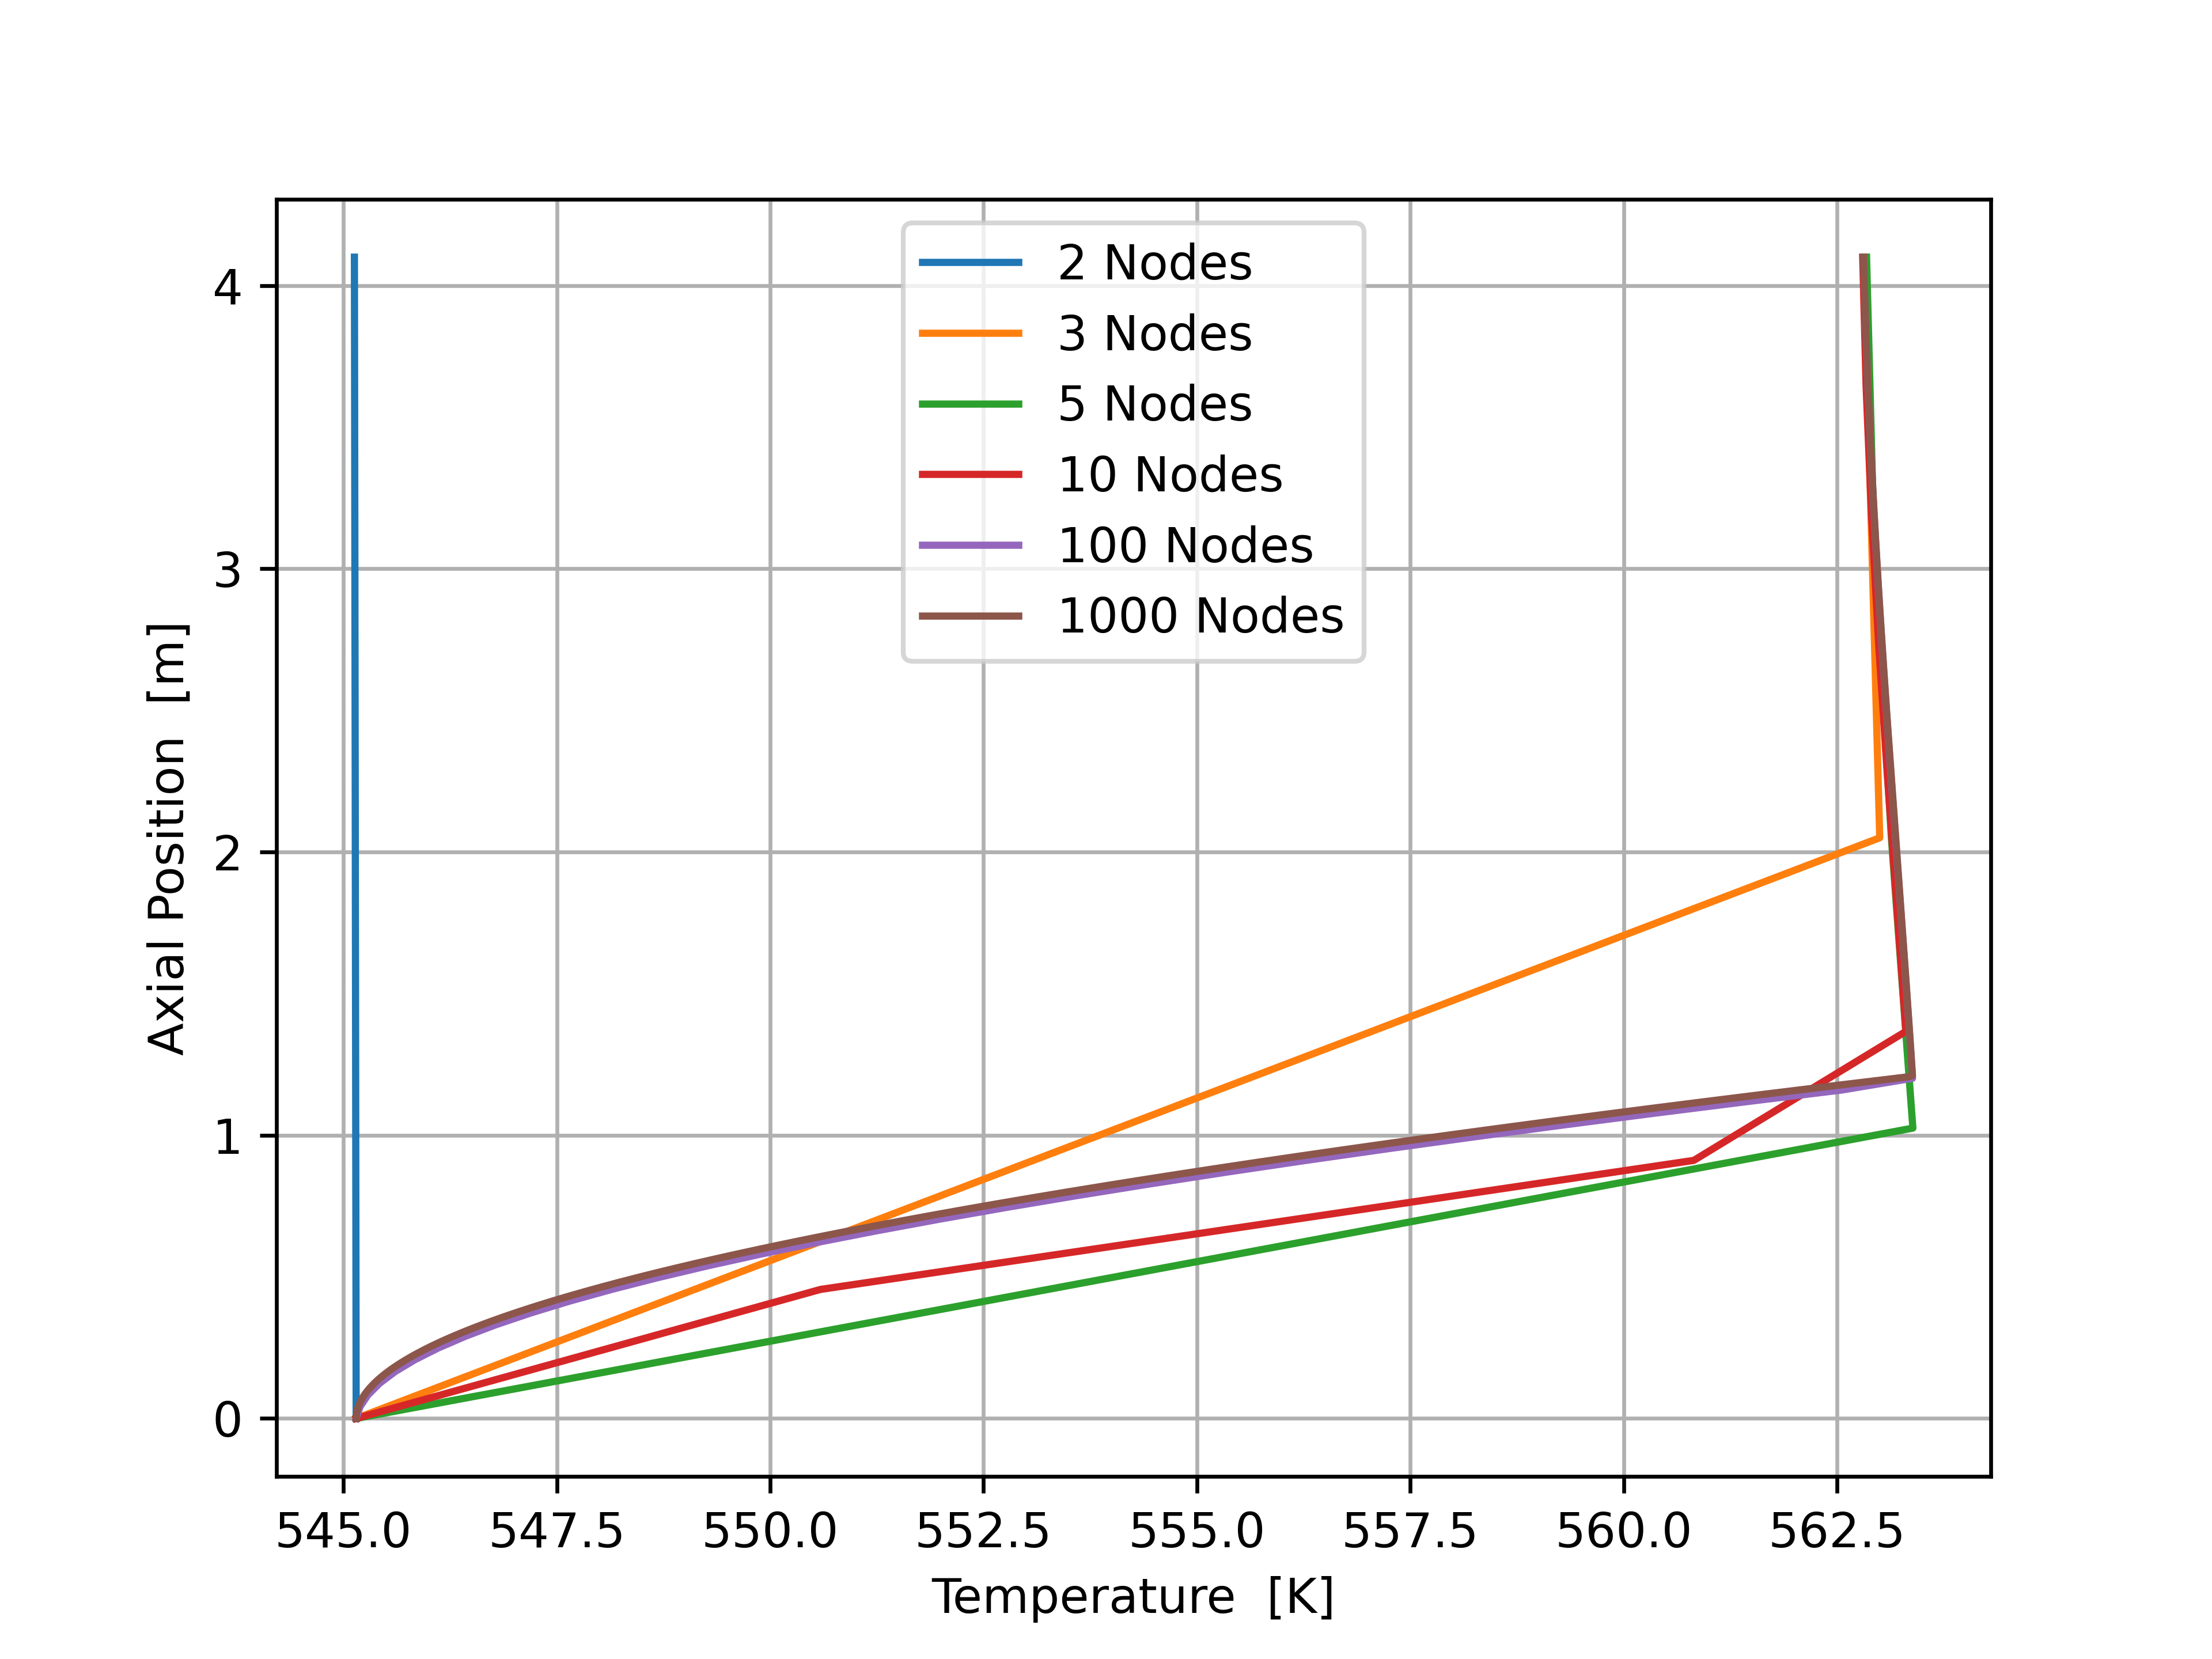
\includegraphics[width=0.5\linewidth]{BWRplots/mesh.png}
    \caption{Mesh convergence of the coolant temperature for the BWR}
    \label{fig:bwrmesh}
\end{figure}

With an appropriate mesh size selected, we know move onto the temperature distributions. Firstly, the fluid saturation temperature as a function of axial position along the channel is presented in Figure \ref{fig:bwrcoolant}. Next, the inner and outer clad surface temperatures as a function of axial position is presented in \ref{fig:bwrclad}. The locations of the onset of nucleate boiling and saturated boiling were 0.341 m and 1.208 m, respectively. Finally, the fuel outer surface and center-line temperature as a function of axial position is presented in \ref{fig:bwrfuel}. To continue, the radial temperature profile of the pin at three axial locations are found. The axial locations are at $\frac{H}{4}$, $\frac{H}{2}$, and $z_{max,cl}$, where $z_{max,cl}$ is defined as the location in which the center-line temperature is maximum. These results are presented in Figures \ref{fig:bwrh4}, \ref{fig:bwrh2}, and \ref{fig:bwrzmax}, respectively, and the maximum center-line temperature occurred at 2.05 meters along the channel. Next, the pressure as a function of axial location is presented in Figure \ref{fig:bwrpressure}. Proximally, the density as a function of axial location is presented in Figure \ref{fig:bwrdensity}. The equilibrium and steam quality, aswell as the void fraction, are presented in Figure \ref{fig:bwrfraction}. 

Next, to present the critical heat flux. First, the critical quality is found using Equation \ref{eq:critx}, is presented in comparison to the quality for different power scalings, all as functions of boiling length, in Figure \ref{fig:bwrcritx}. The scaling factor that yielded the tangent line was 1.17326, and thus the critical power ratio is 1.17326, which is lower than thermal design criteria of 1.2. Next, the DNB was investigated. Again utilizing Equation \ref{eq:dnbr}, the critical and operating heat fluxes are presented in Figure \ref{fig:bwrdnb}, and the resulting ratio is presented in Figure \ref{fig:bwrdnbr}. For the BWR design, the minimum DNBR is found to be 1.2873, below the thermal design criteria of 1.3.

\begin{figure}[!hp!]
    \begin{minipage}[b]{.45\linewidth}
    \centering
        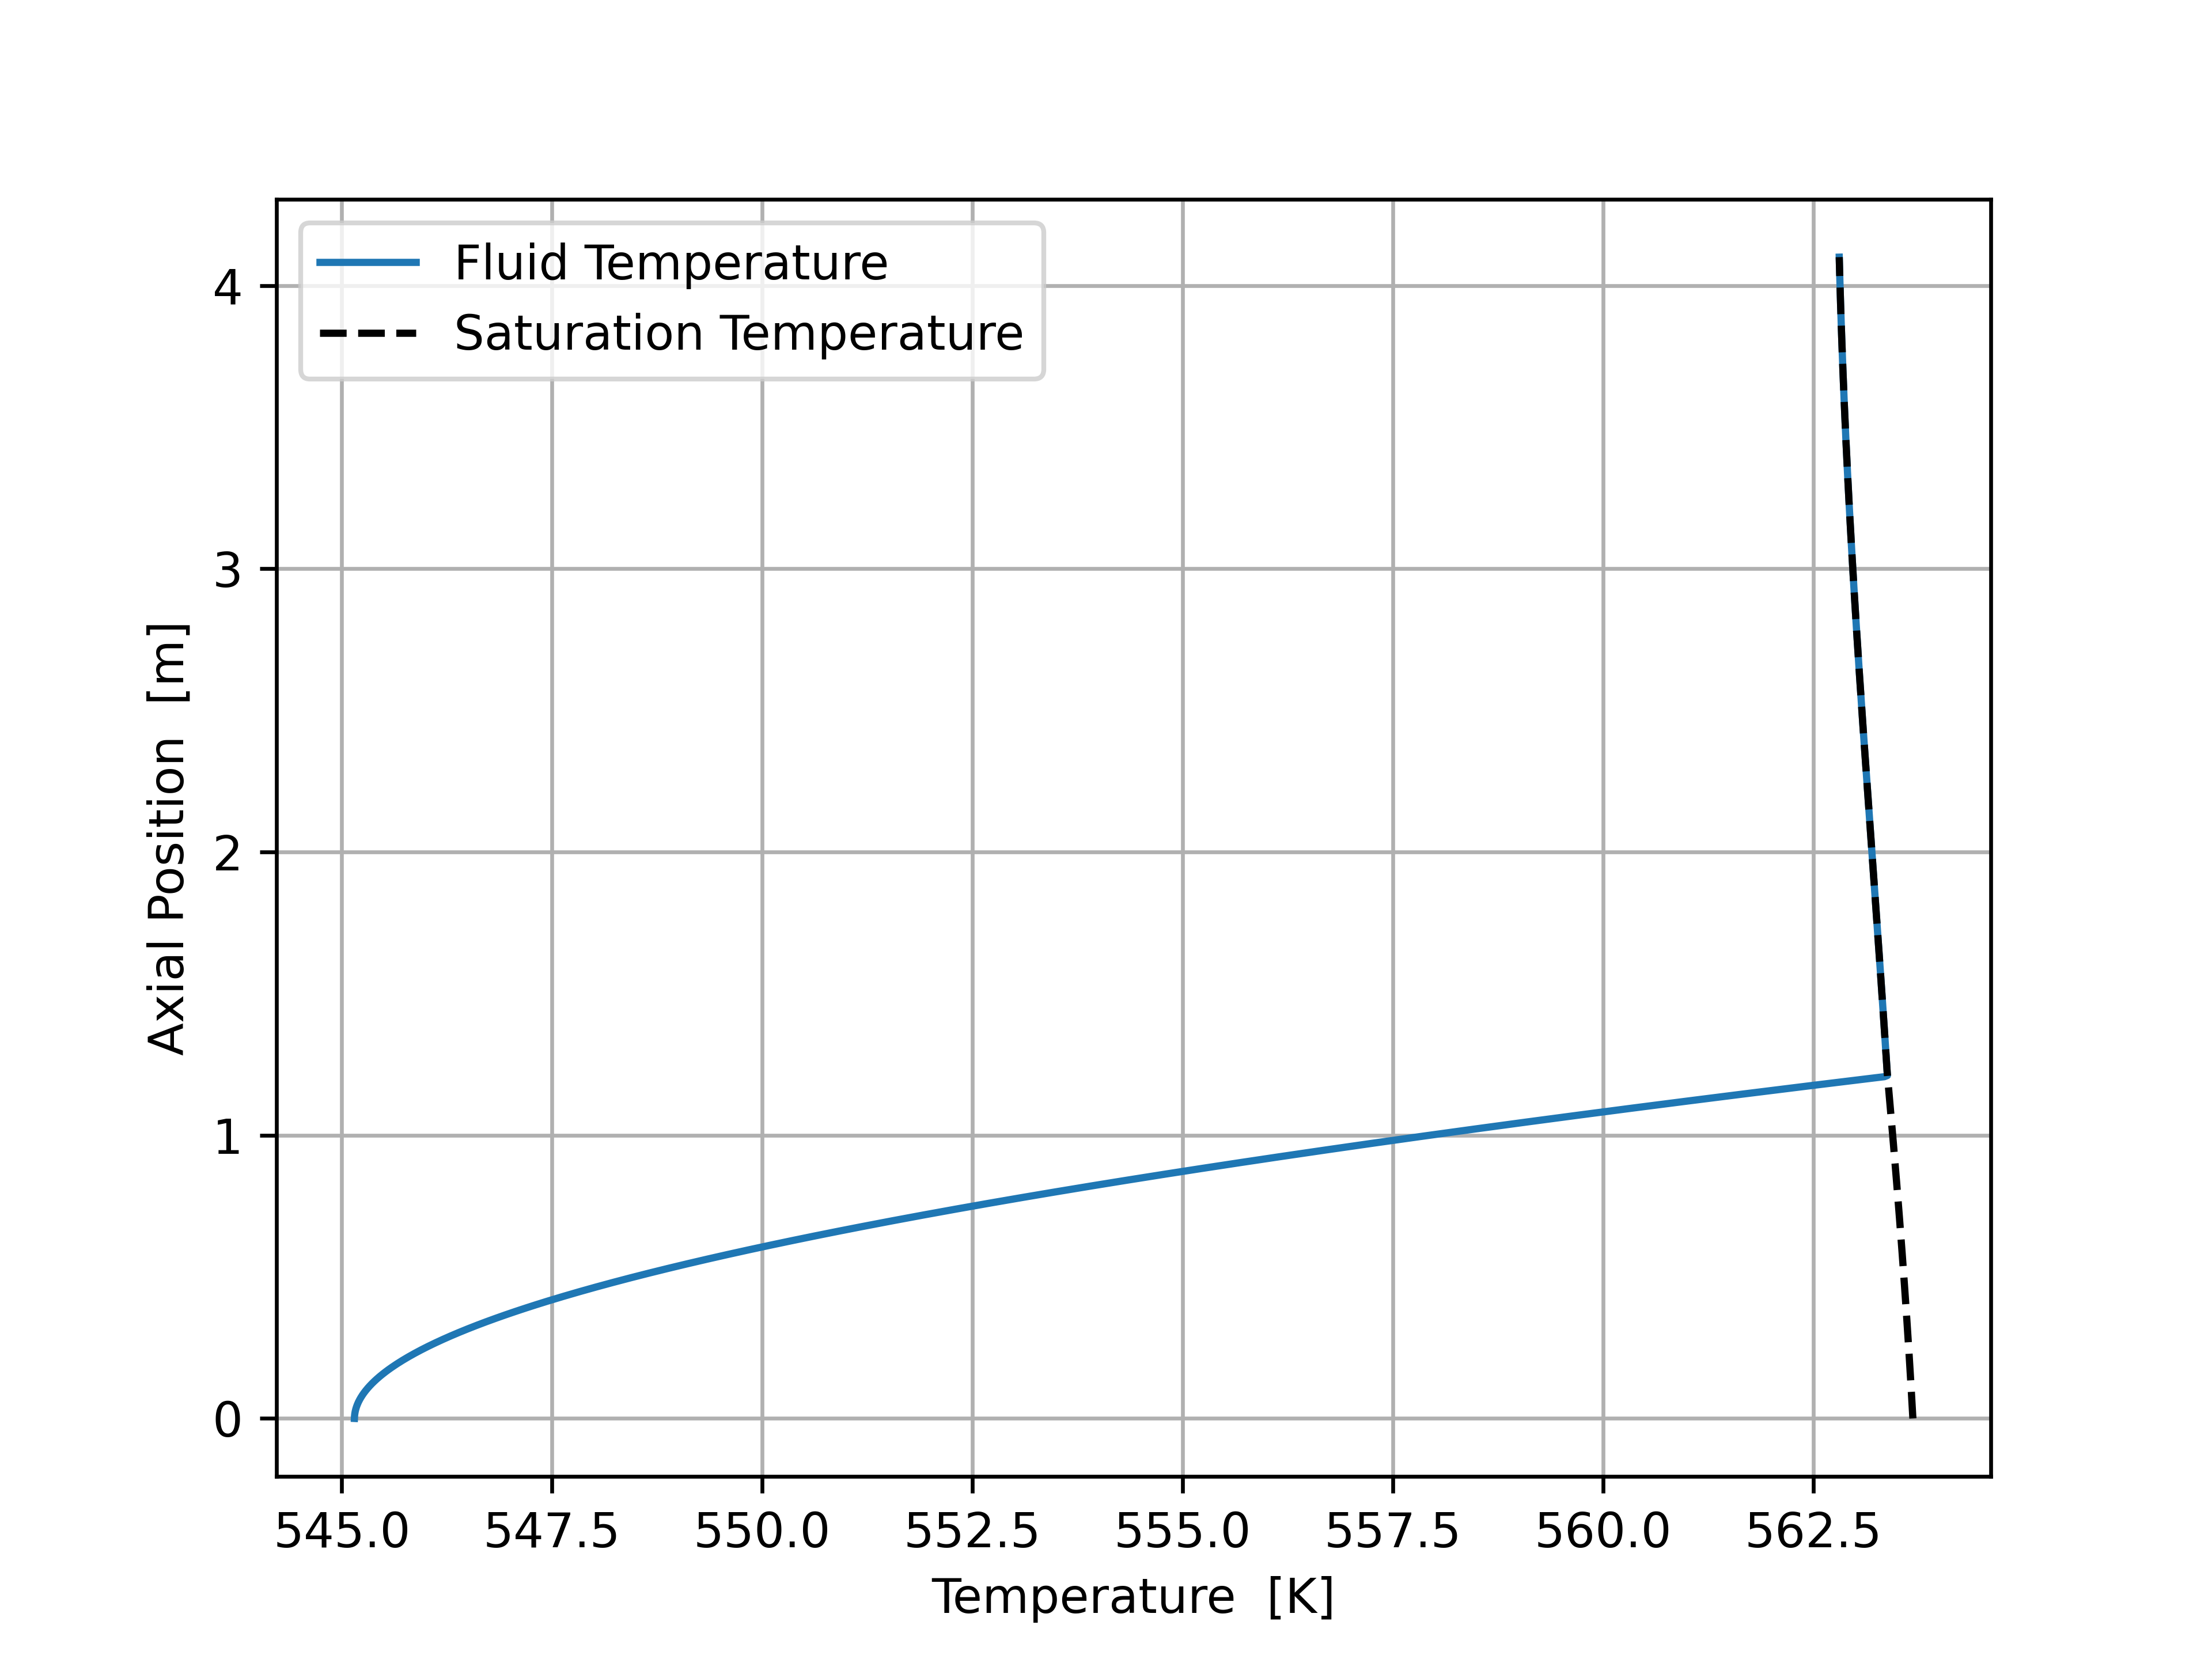
\includegraphics[width=\linewidth]{BWRplots/tfluid.png}
        \caption{BWR coolant temperature as a function of axial location}
        \label{fig:bwrcoolant}
        \vspace{4ex}
    \end{minipage}
    \begin{minipage}[b]{.45\linewidth}
    \centering
        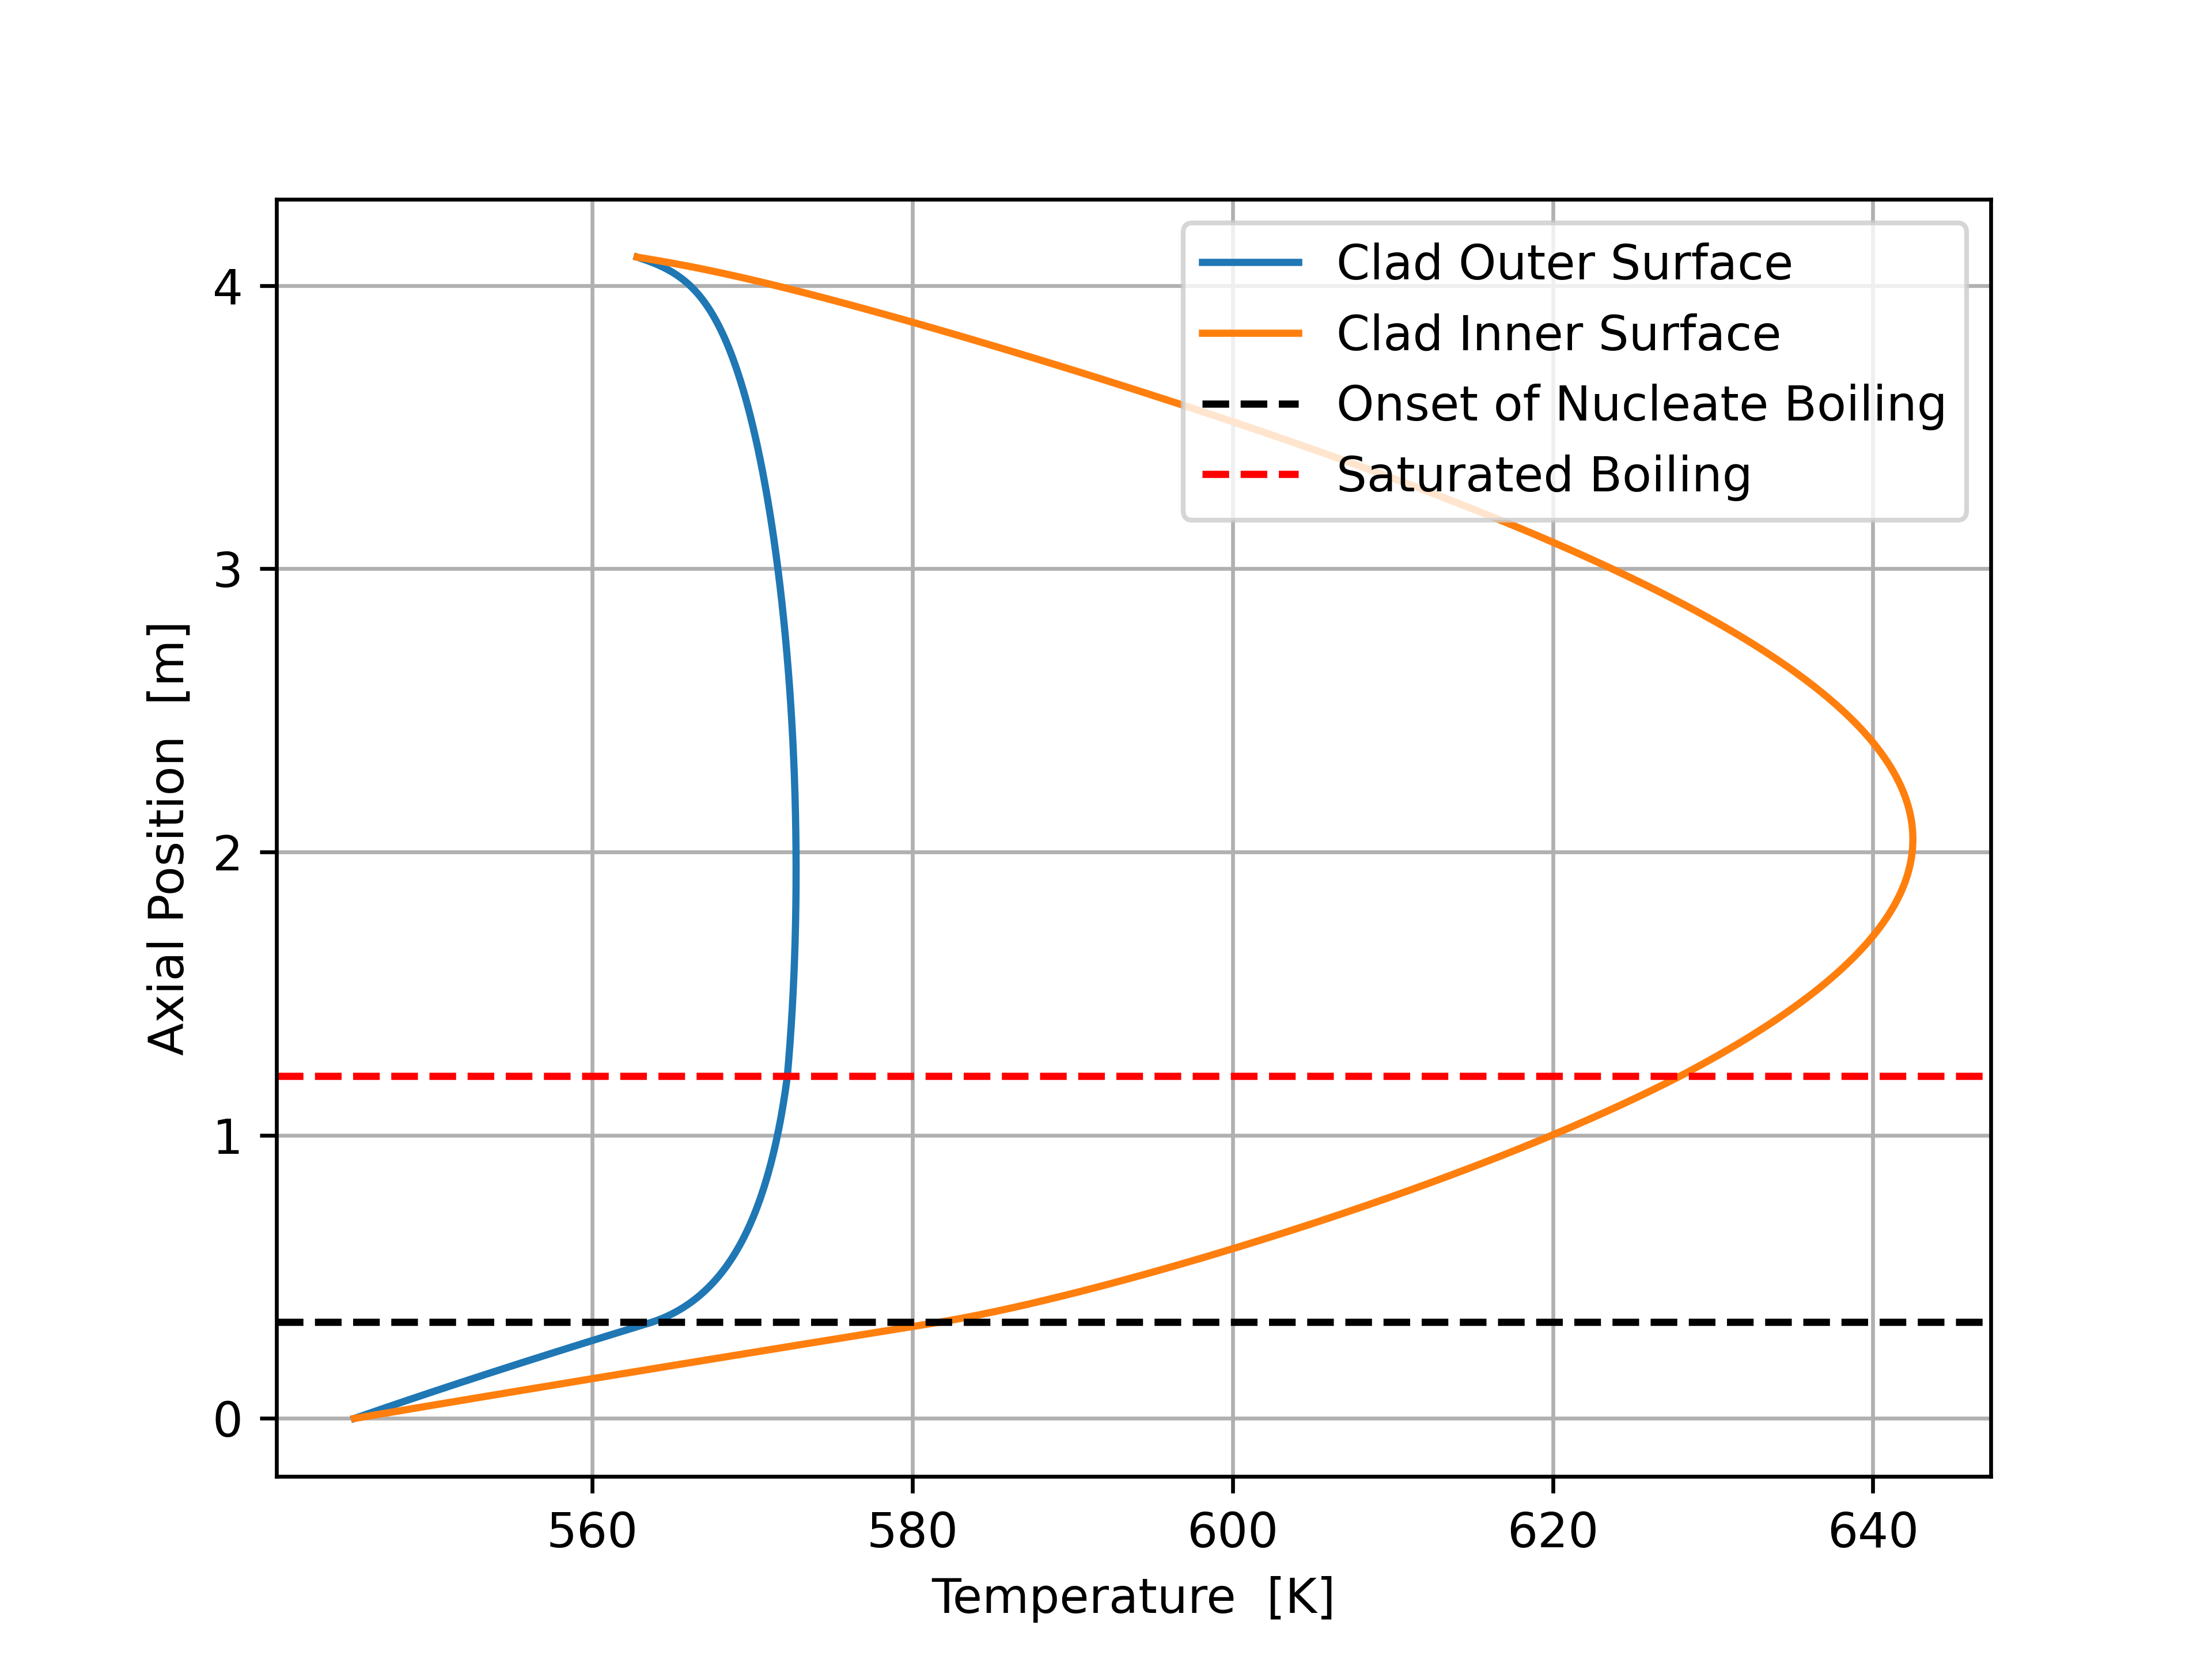
\includegraphics[width=\linewidth]{BWRplots/tclad.png}
        \caption{BWR clad temperature as a function of axial location}
        \label{fig:bwrclad}
        \vspace{4ex}
    \end{minipage}
    \begin{minipage}[b]{.45\linewidth}
    \centering
        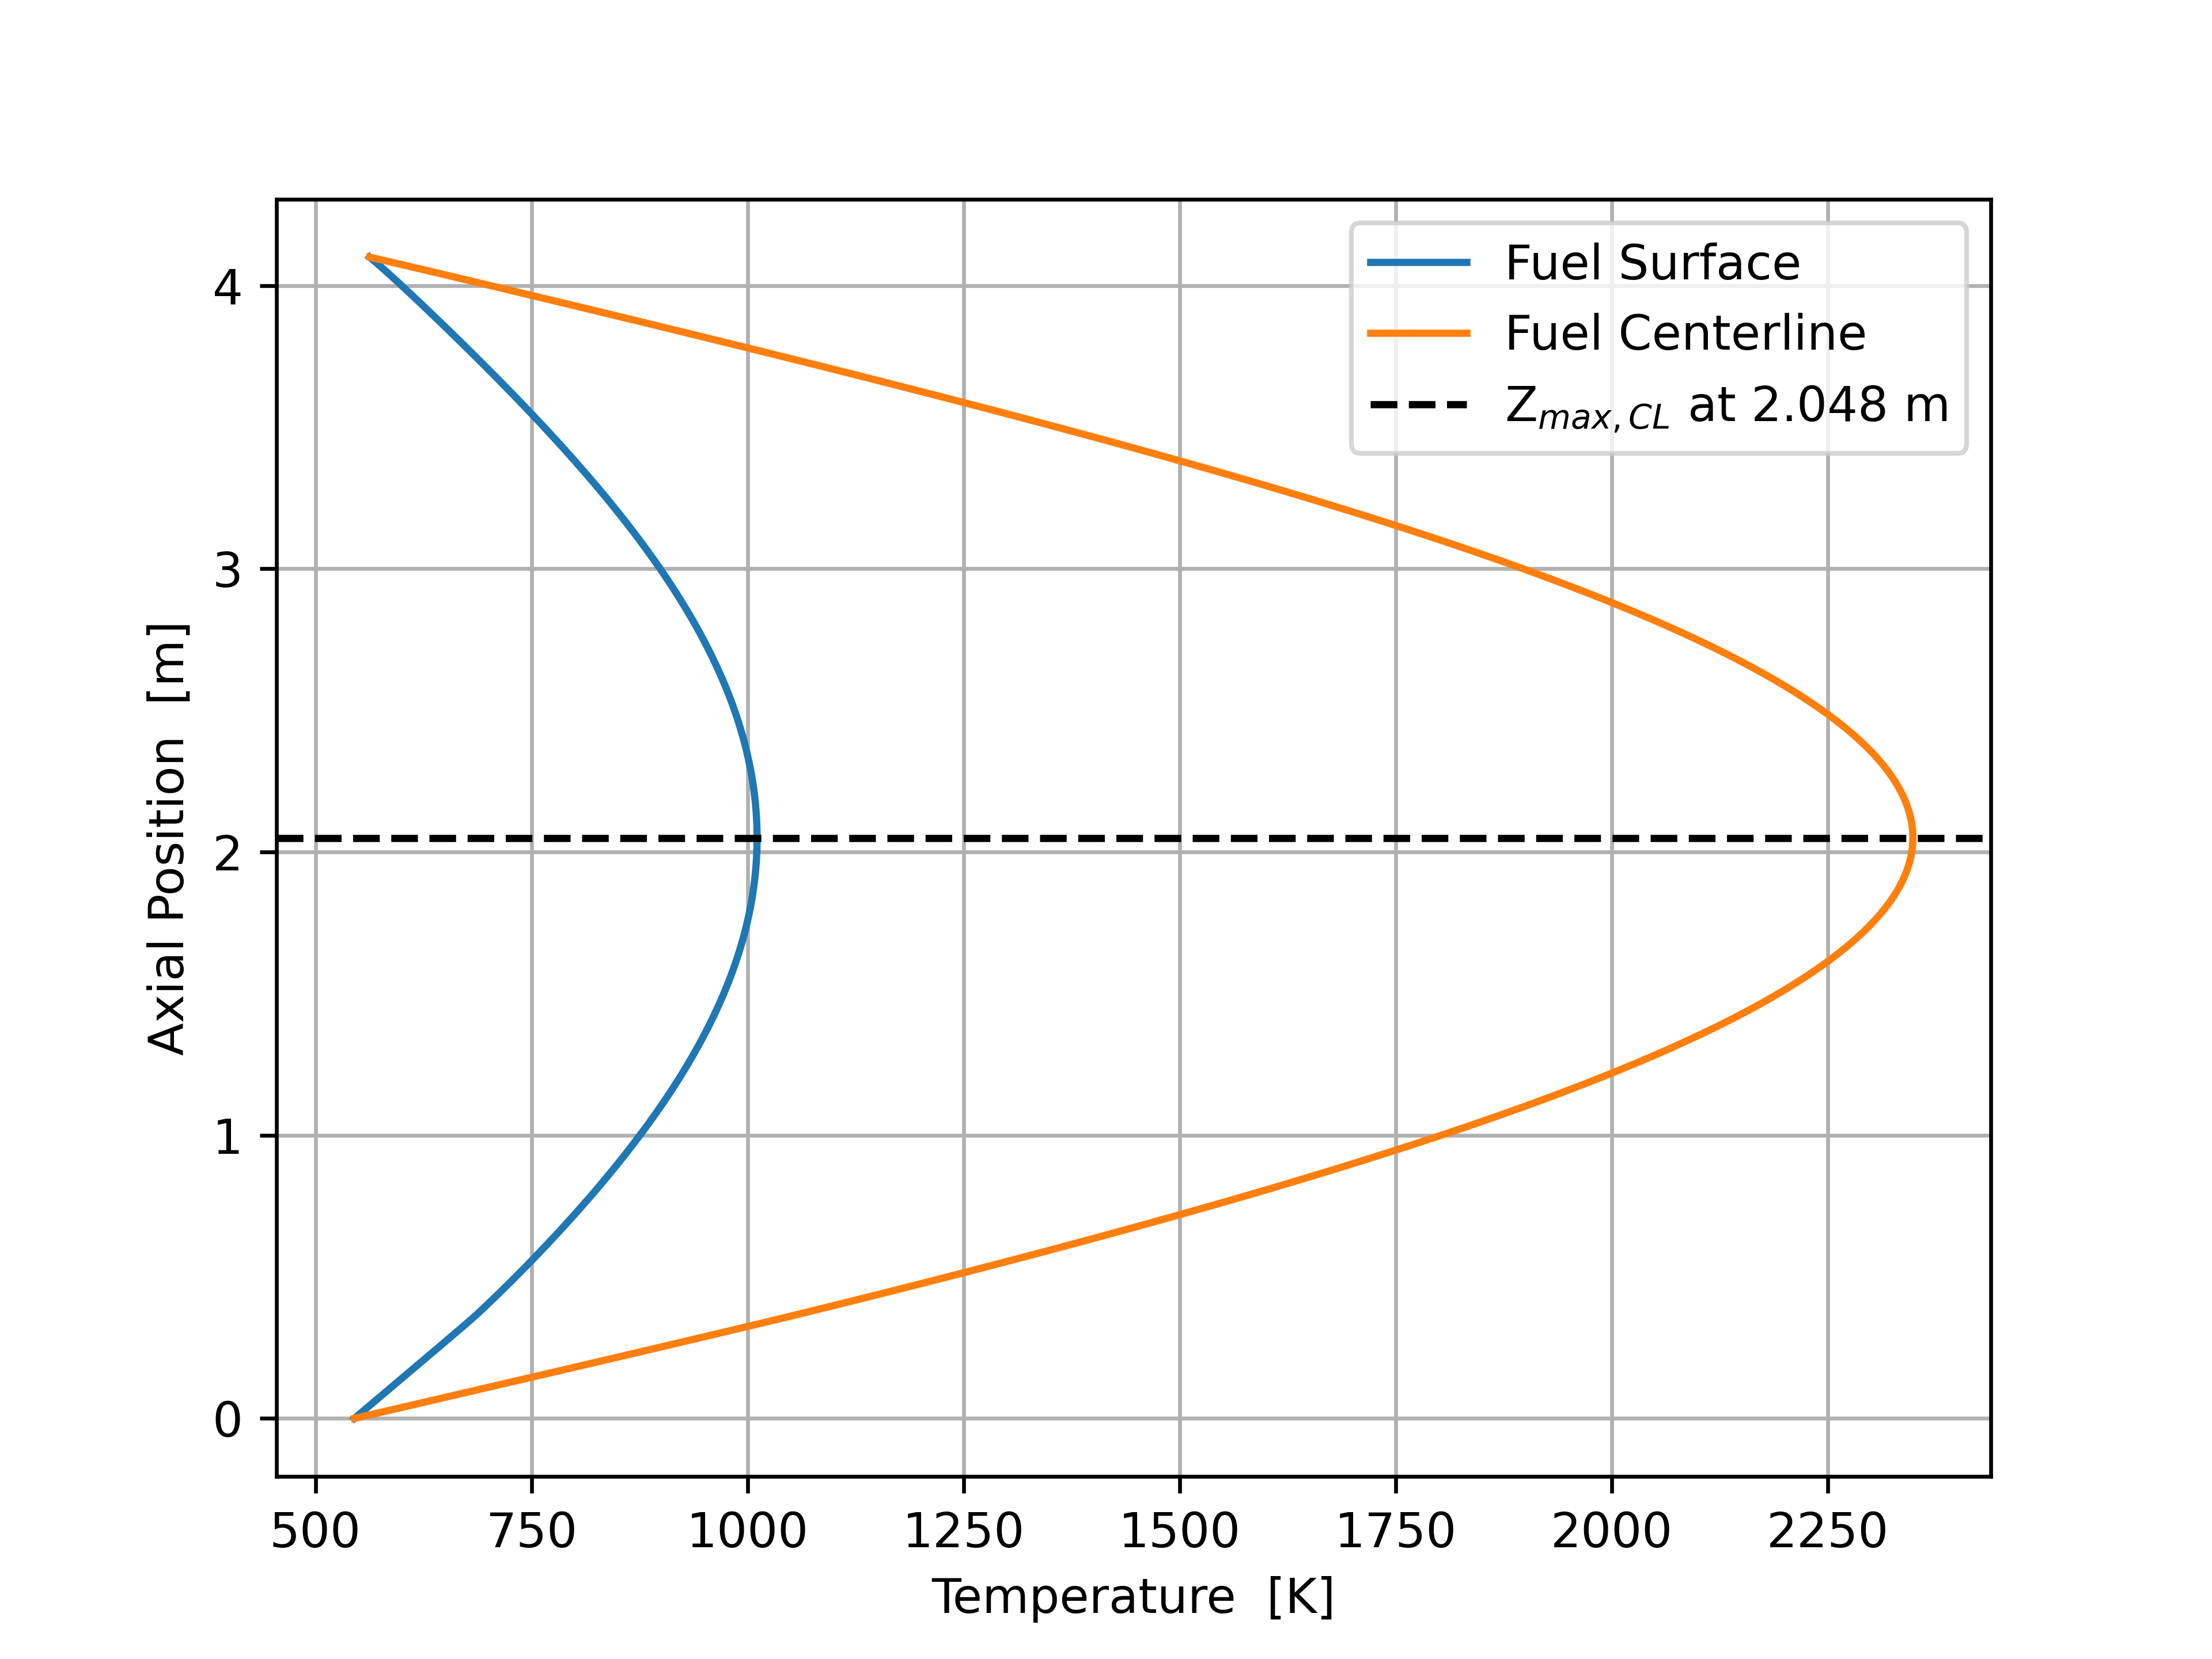
\includegraphics[width=\linewidth]{BWRplots/tfuel.png}
        \caption{BWR fuel temperature as a function of axial location}
        \label{fig:bwrfuel}
        \vspace{4ex}
    \end{minipage}
    \begin{minipage}[b]{.45\linewidth}
    \centering
        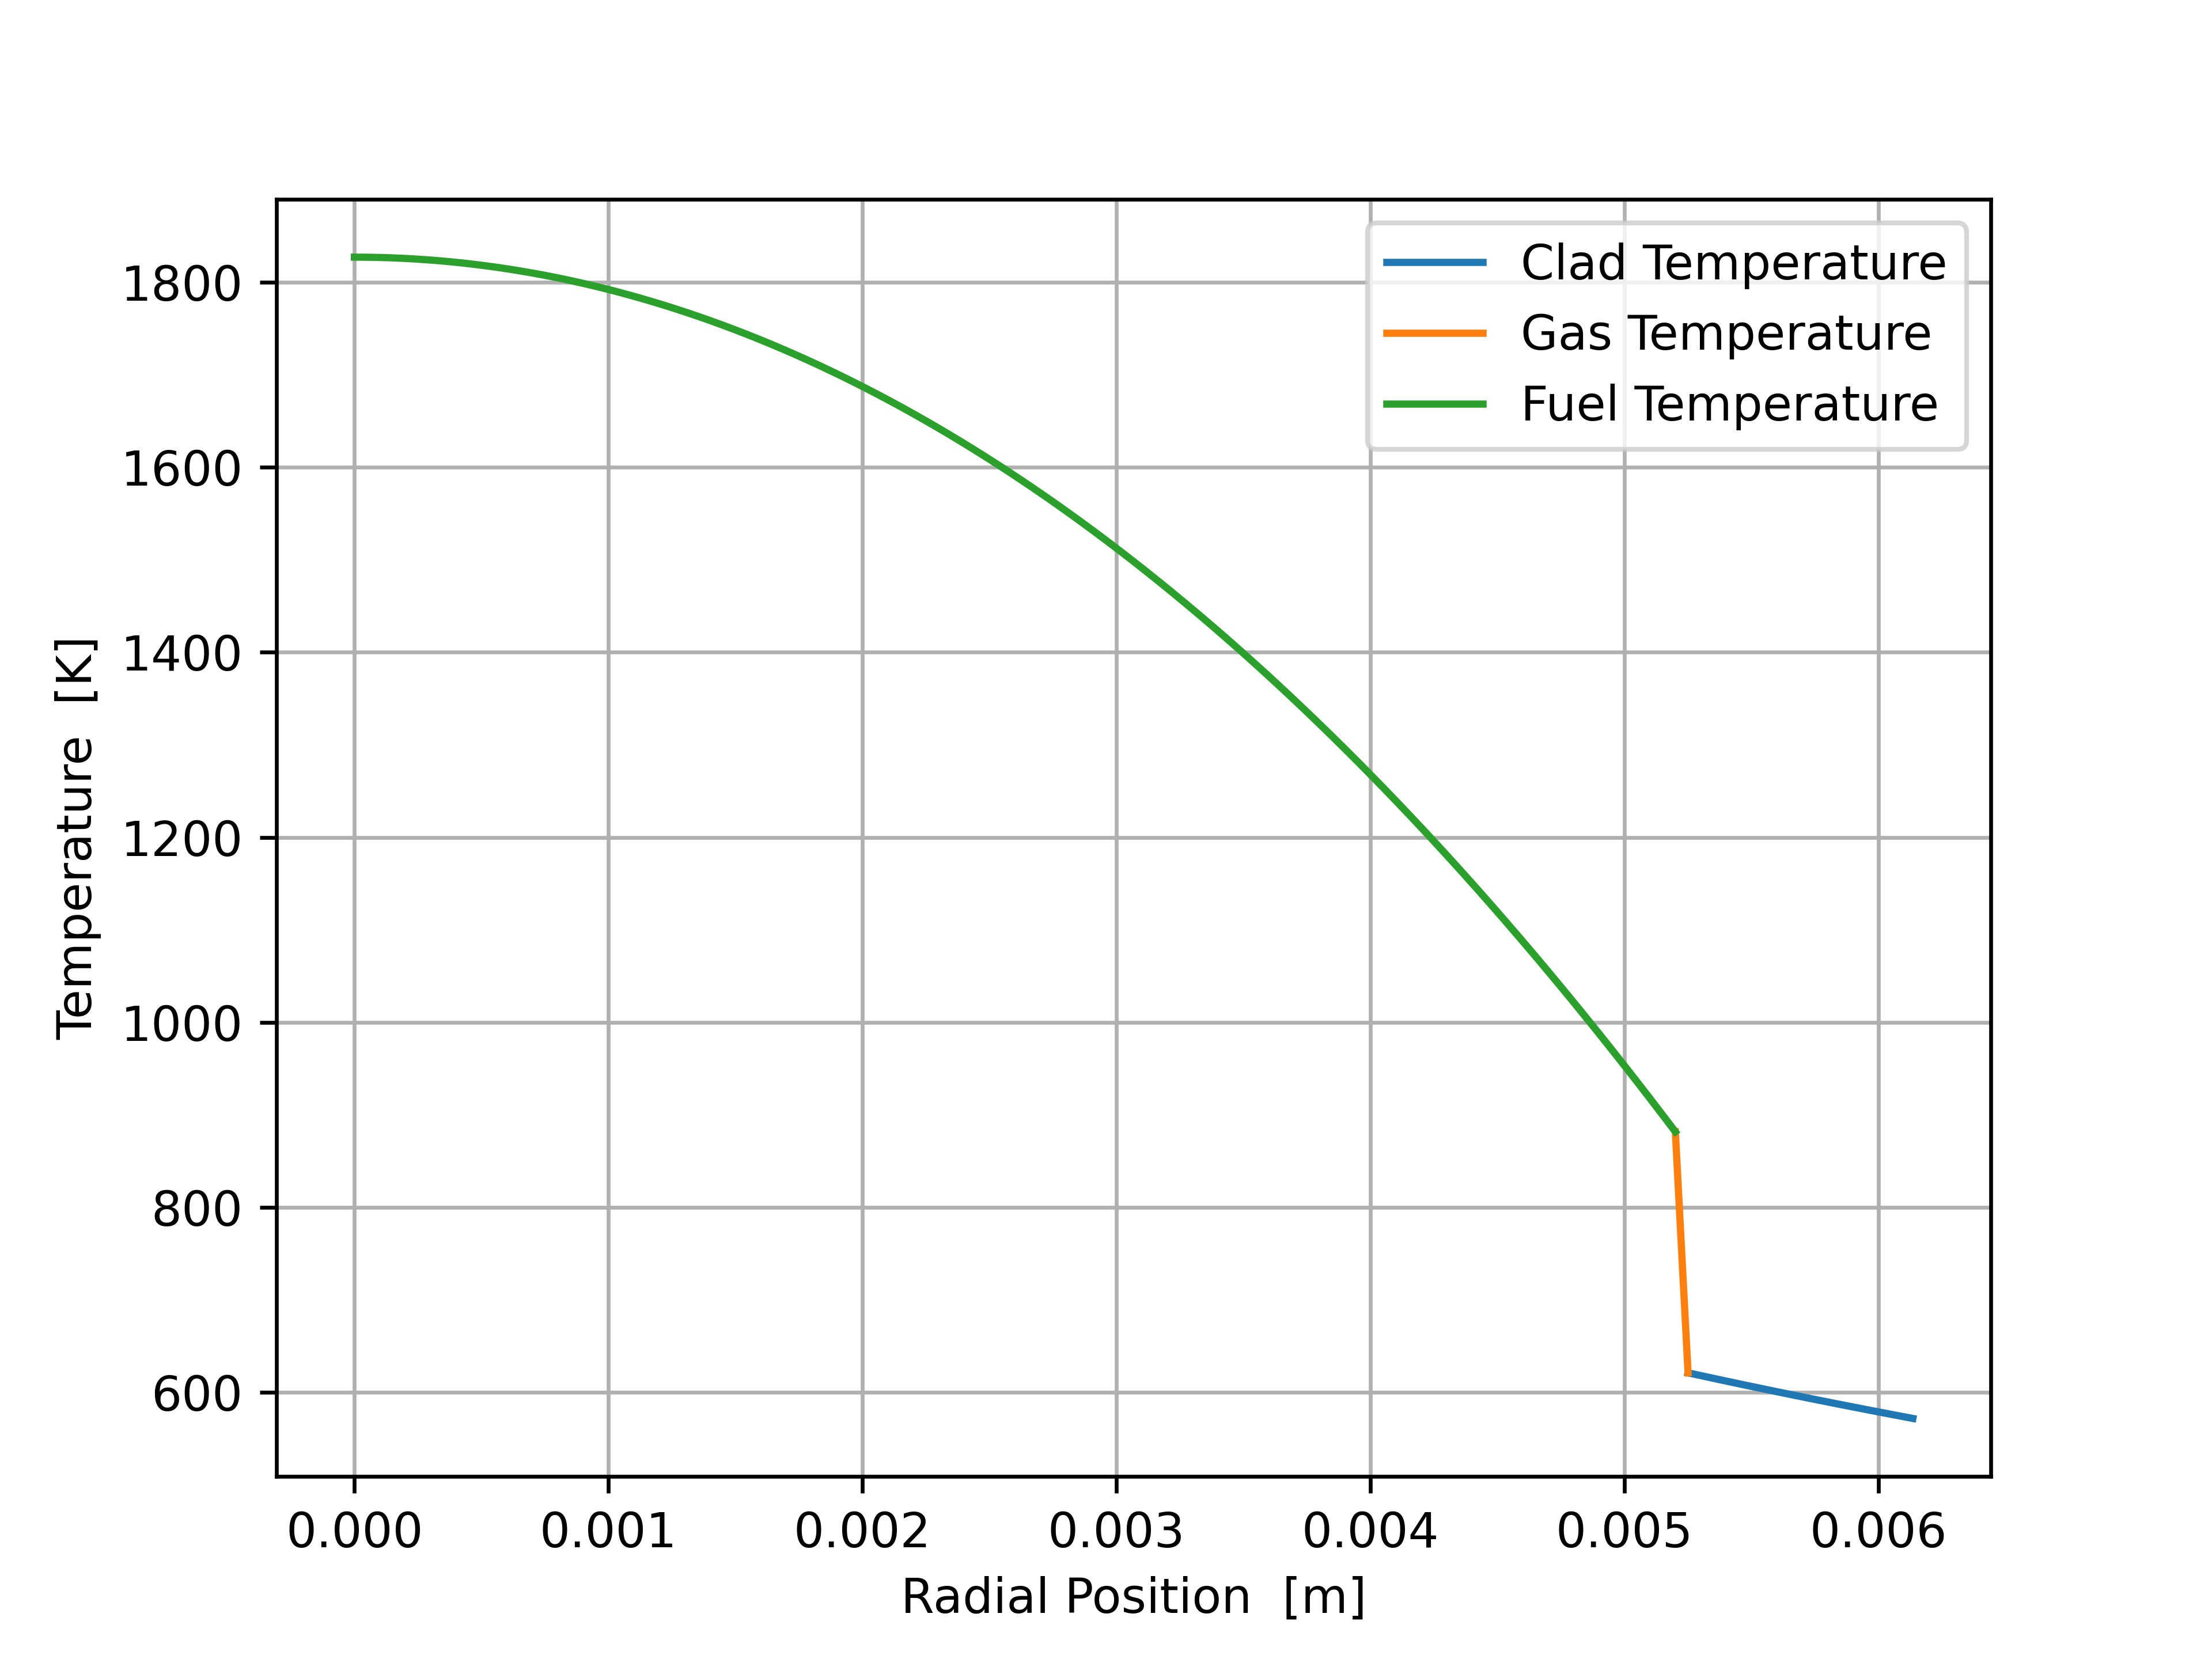
\includegraphics[width=\linewidth]{BWRplots/r-at-1.025.png}
        \caption{Radial BWR pin temperature distribution at H = 1.025 m}
        \label{fig:bwrh4}
        \vspace{4ex}
    \end{minipage}
    \begin{minipage}[b]{.45\linewidth}
    \centering
        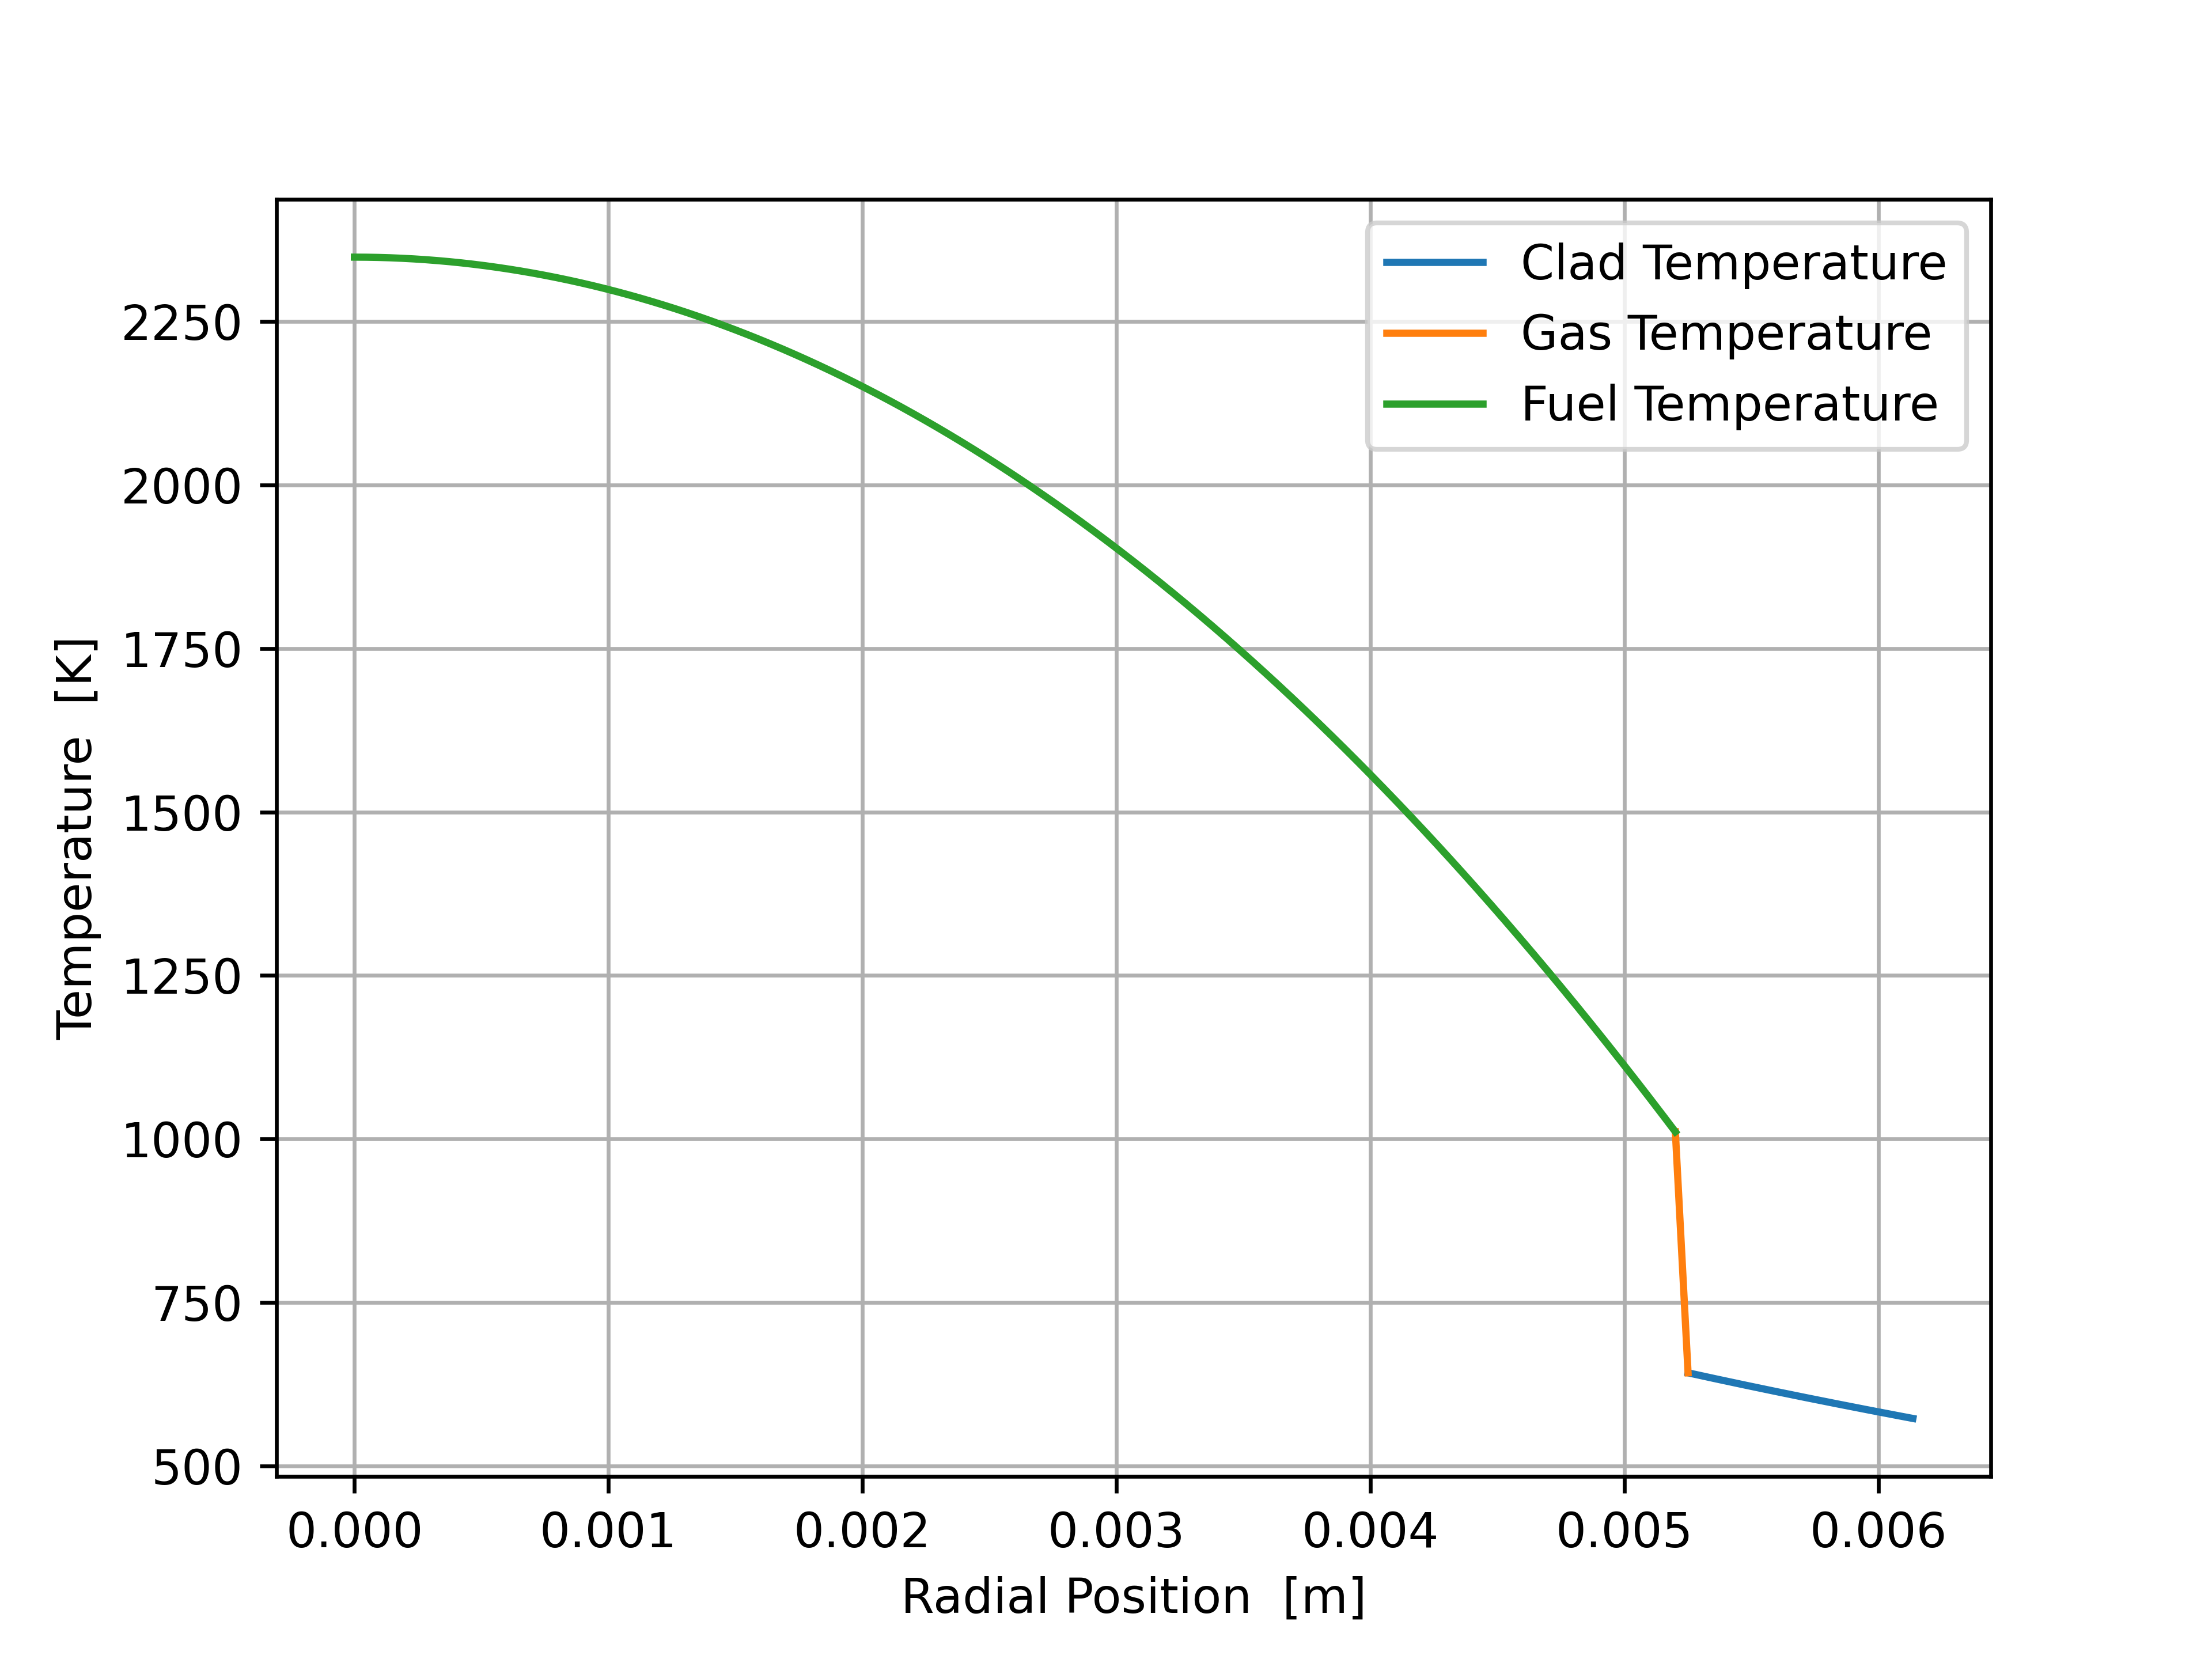
\includegraphics[width=\linewidth]{BWRplots/r-at-2.05.png}
        \caption{Radial BWR pin temperature distribution at H = 2.05 m}
        \label{fig:bwrh2}
        \vspace{4ex}
    \end{minipage}
    \begin{minipage}[b]{.45\linewidth}
    \centering
        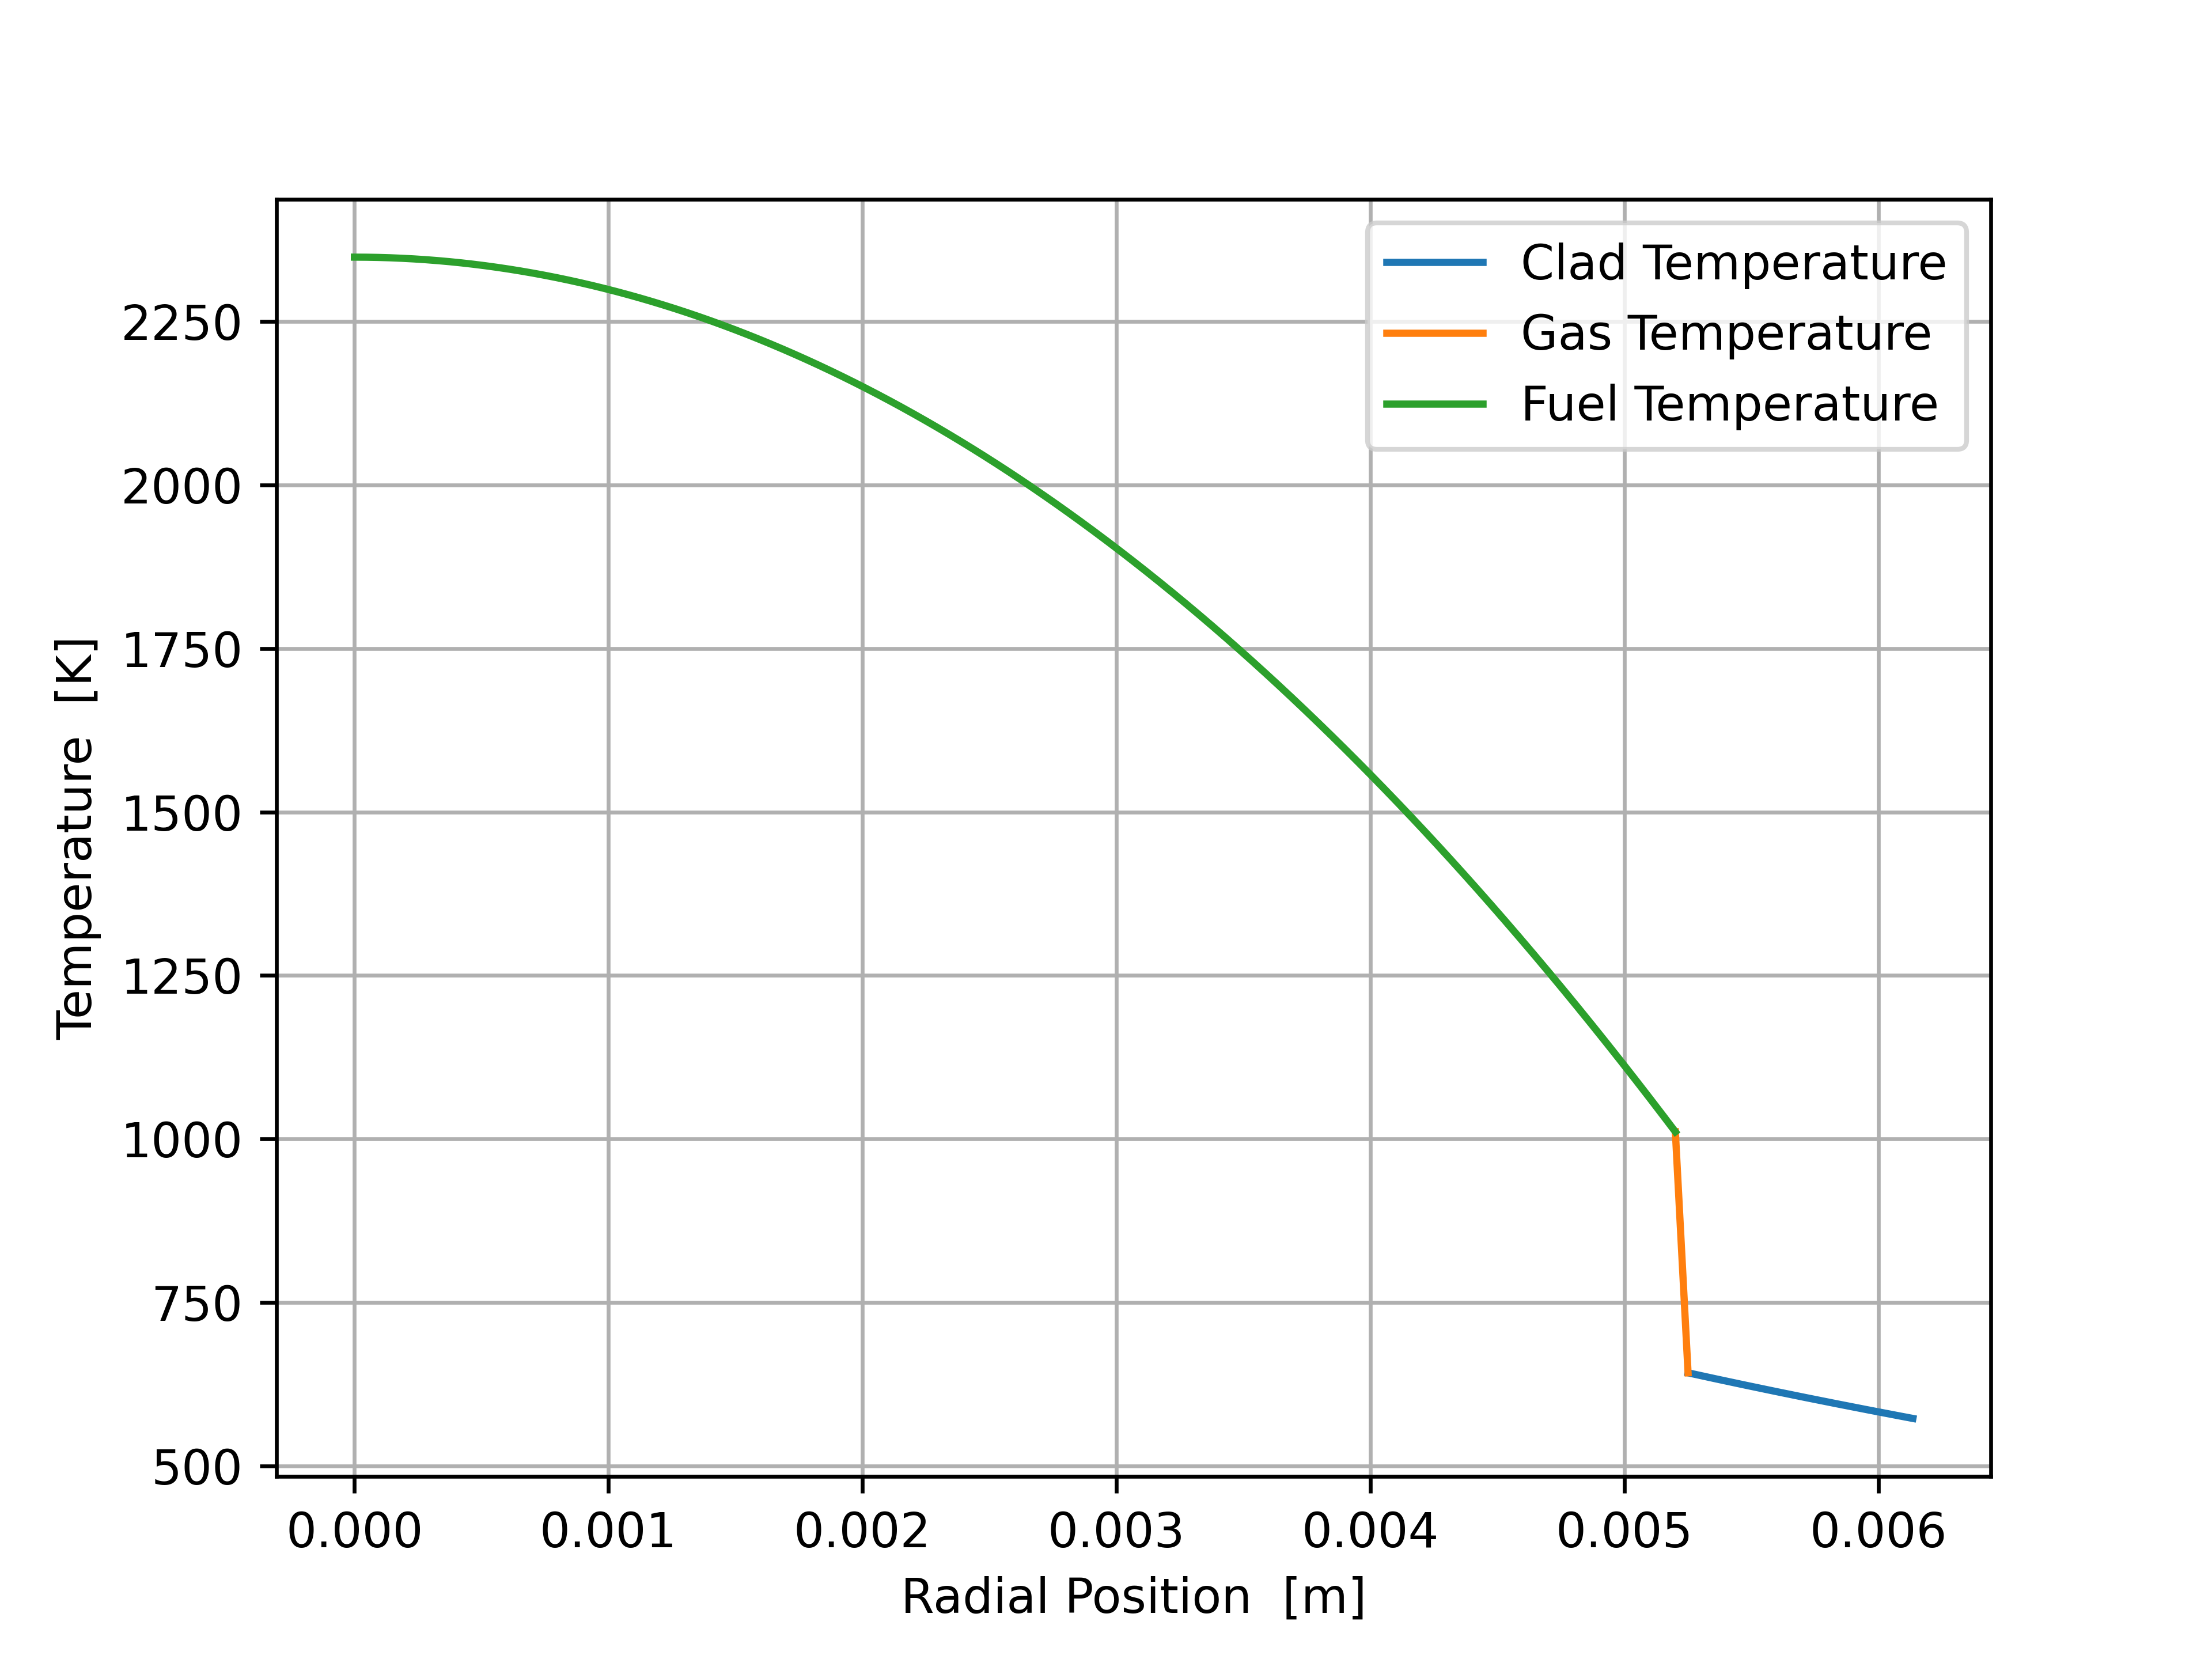
\includegraphics[width=\linewidth]{BWRplots/r-at-2.047947947947948.png}
        \caption{Radial BWR pin temperature distribution at H = 2.05 m}
        \label{fig:bwrzmax}
        \vspace{4ex}
    \end{minipage}
\end{figure}

\begin{figure}[!hp!]
    \centering
    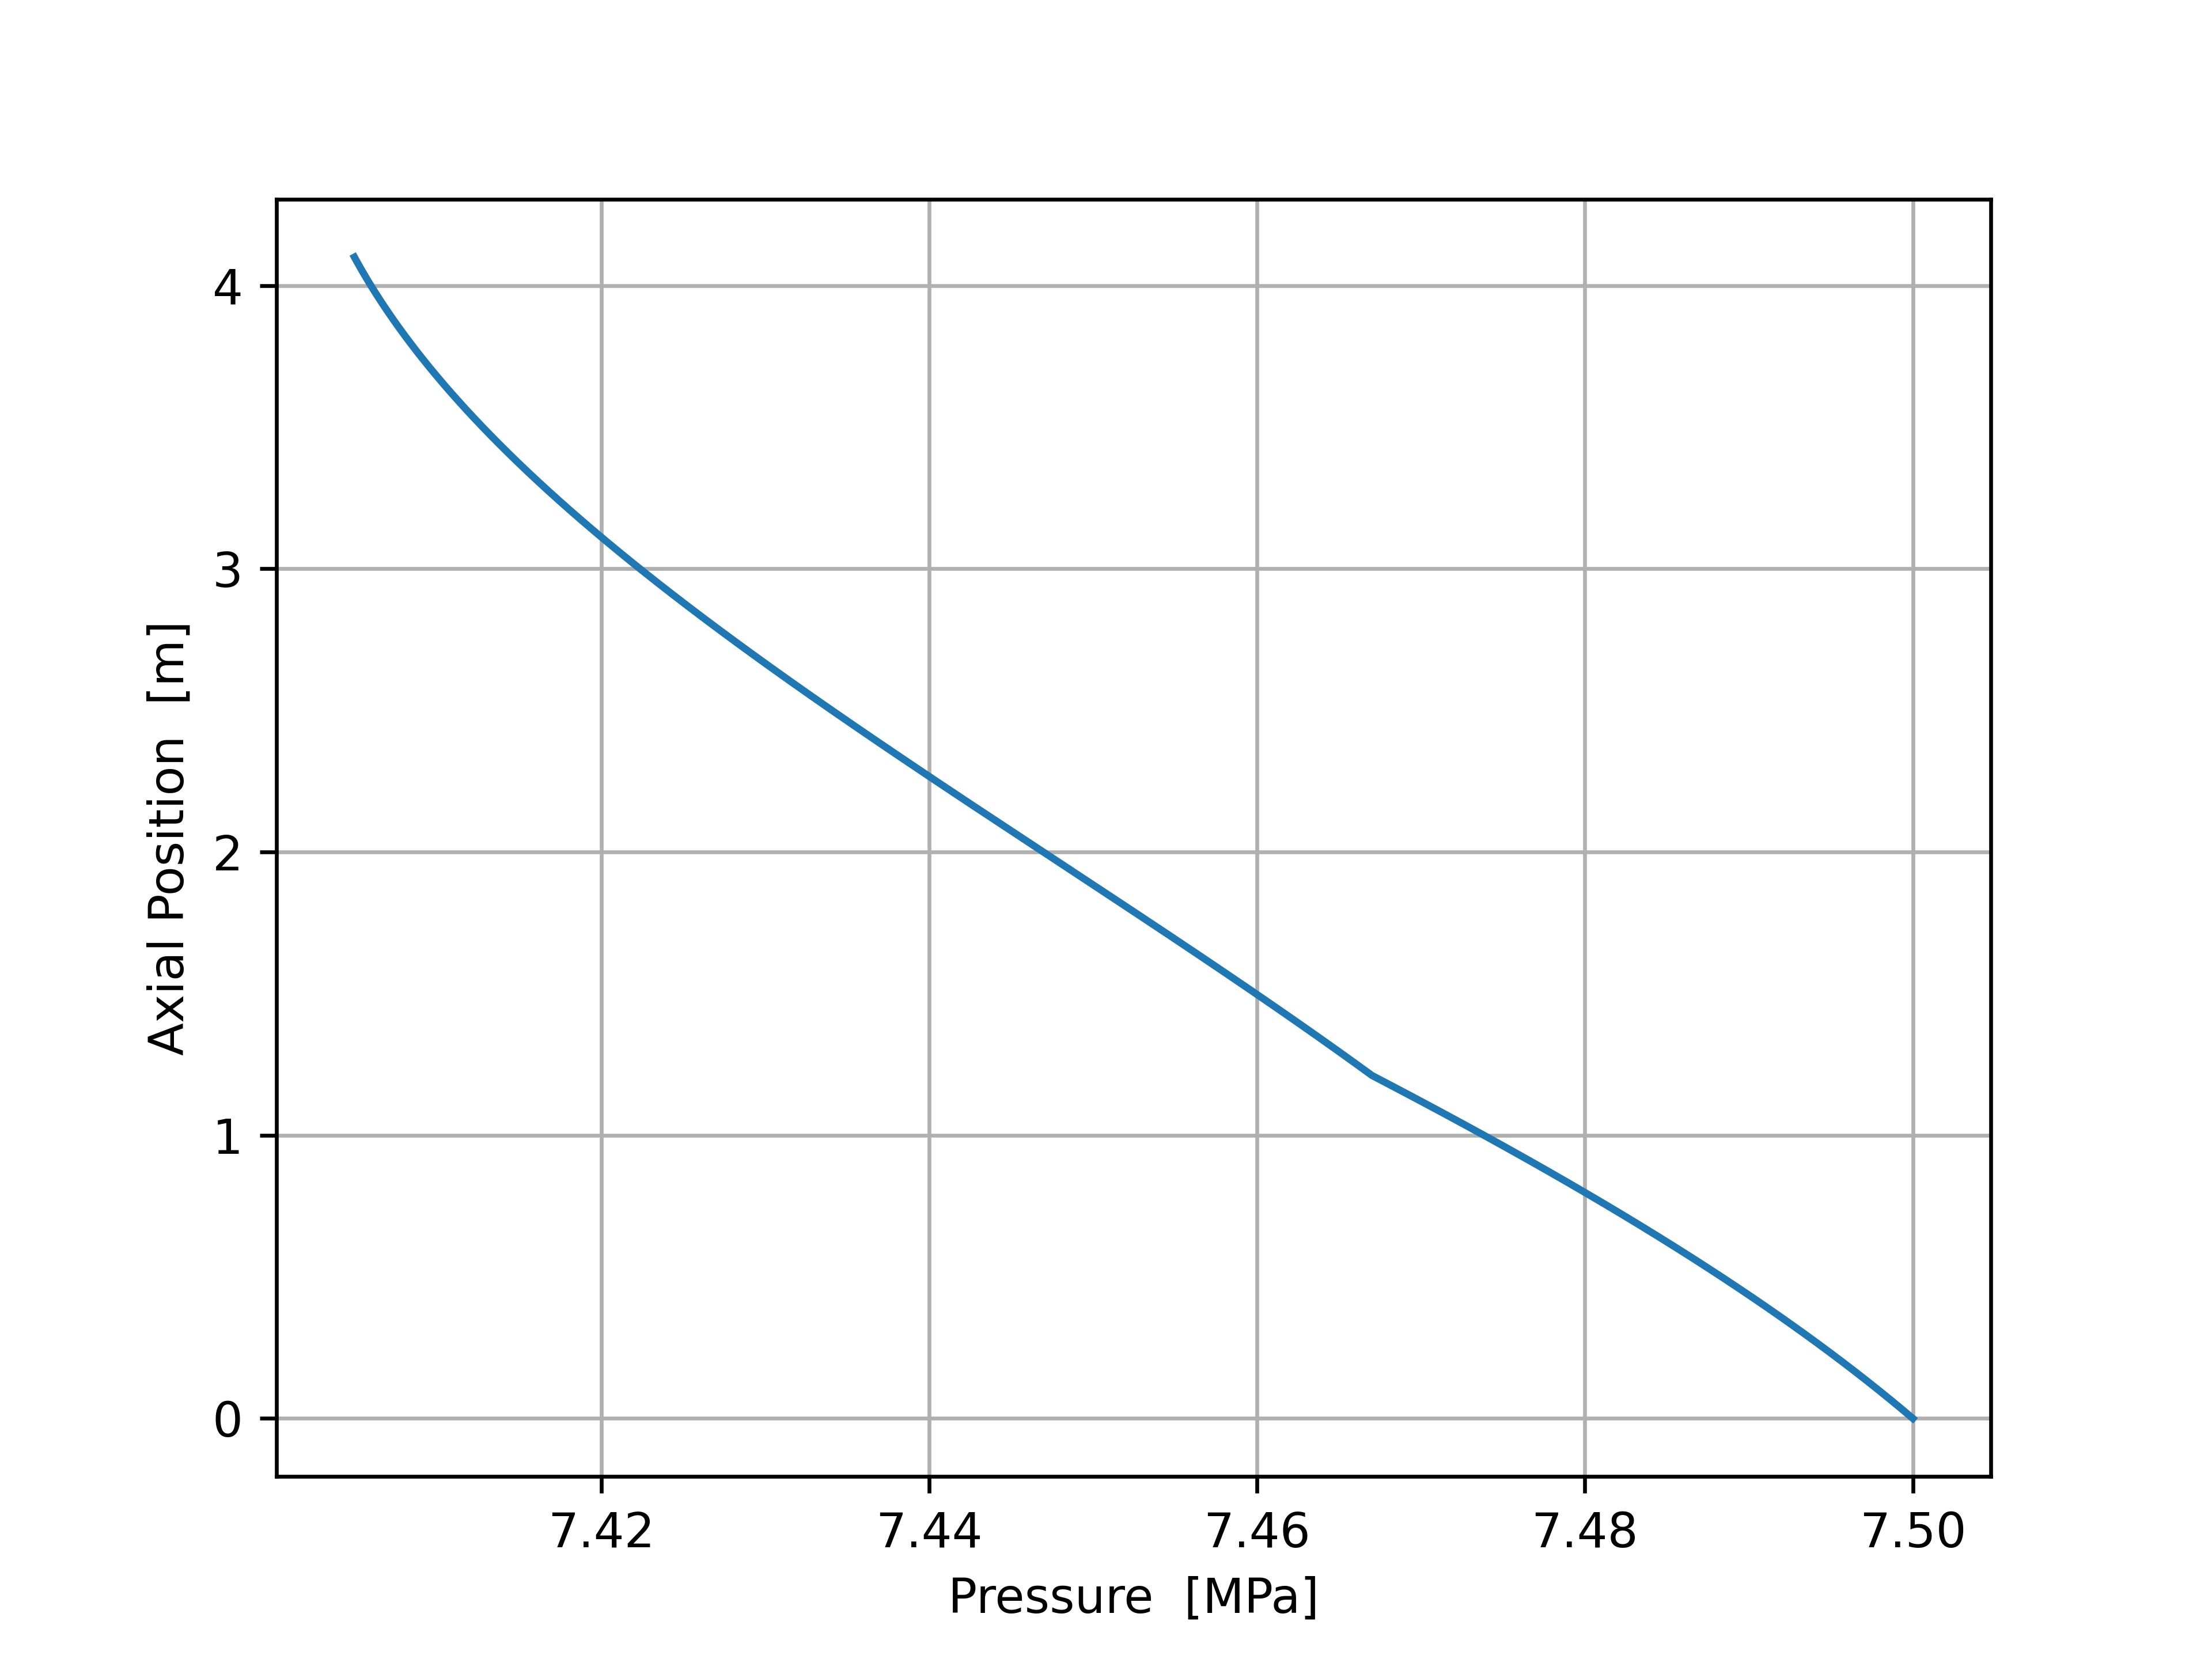
\includegraphics[width=0.5\linewidth]{BWRplots/pressure.png}
    \caption{BWR pressure as a function of axial location}
    \label{fig:bwrpressure}
\end{figure}

\begin{figure}[!hp!]
    \begin{minipage}[b]{.45\linewidth}
        \centering
        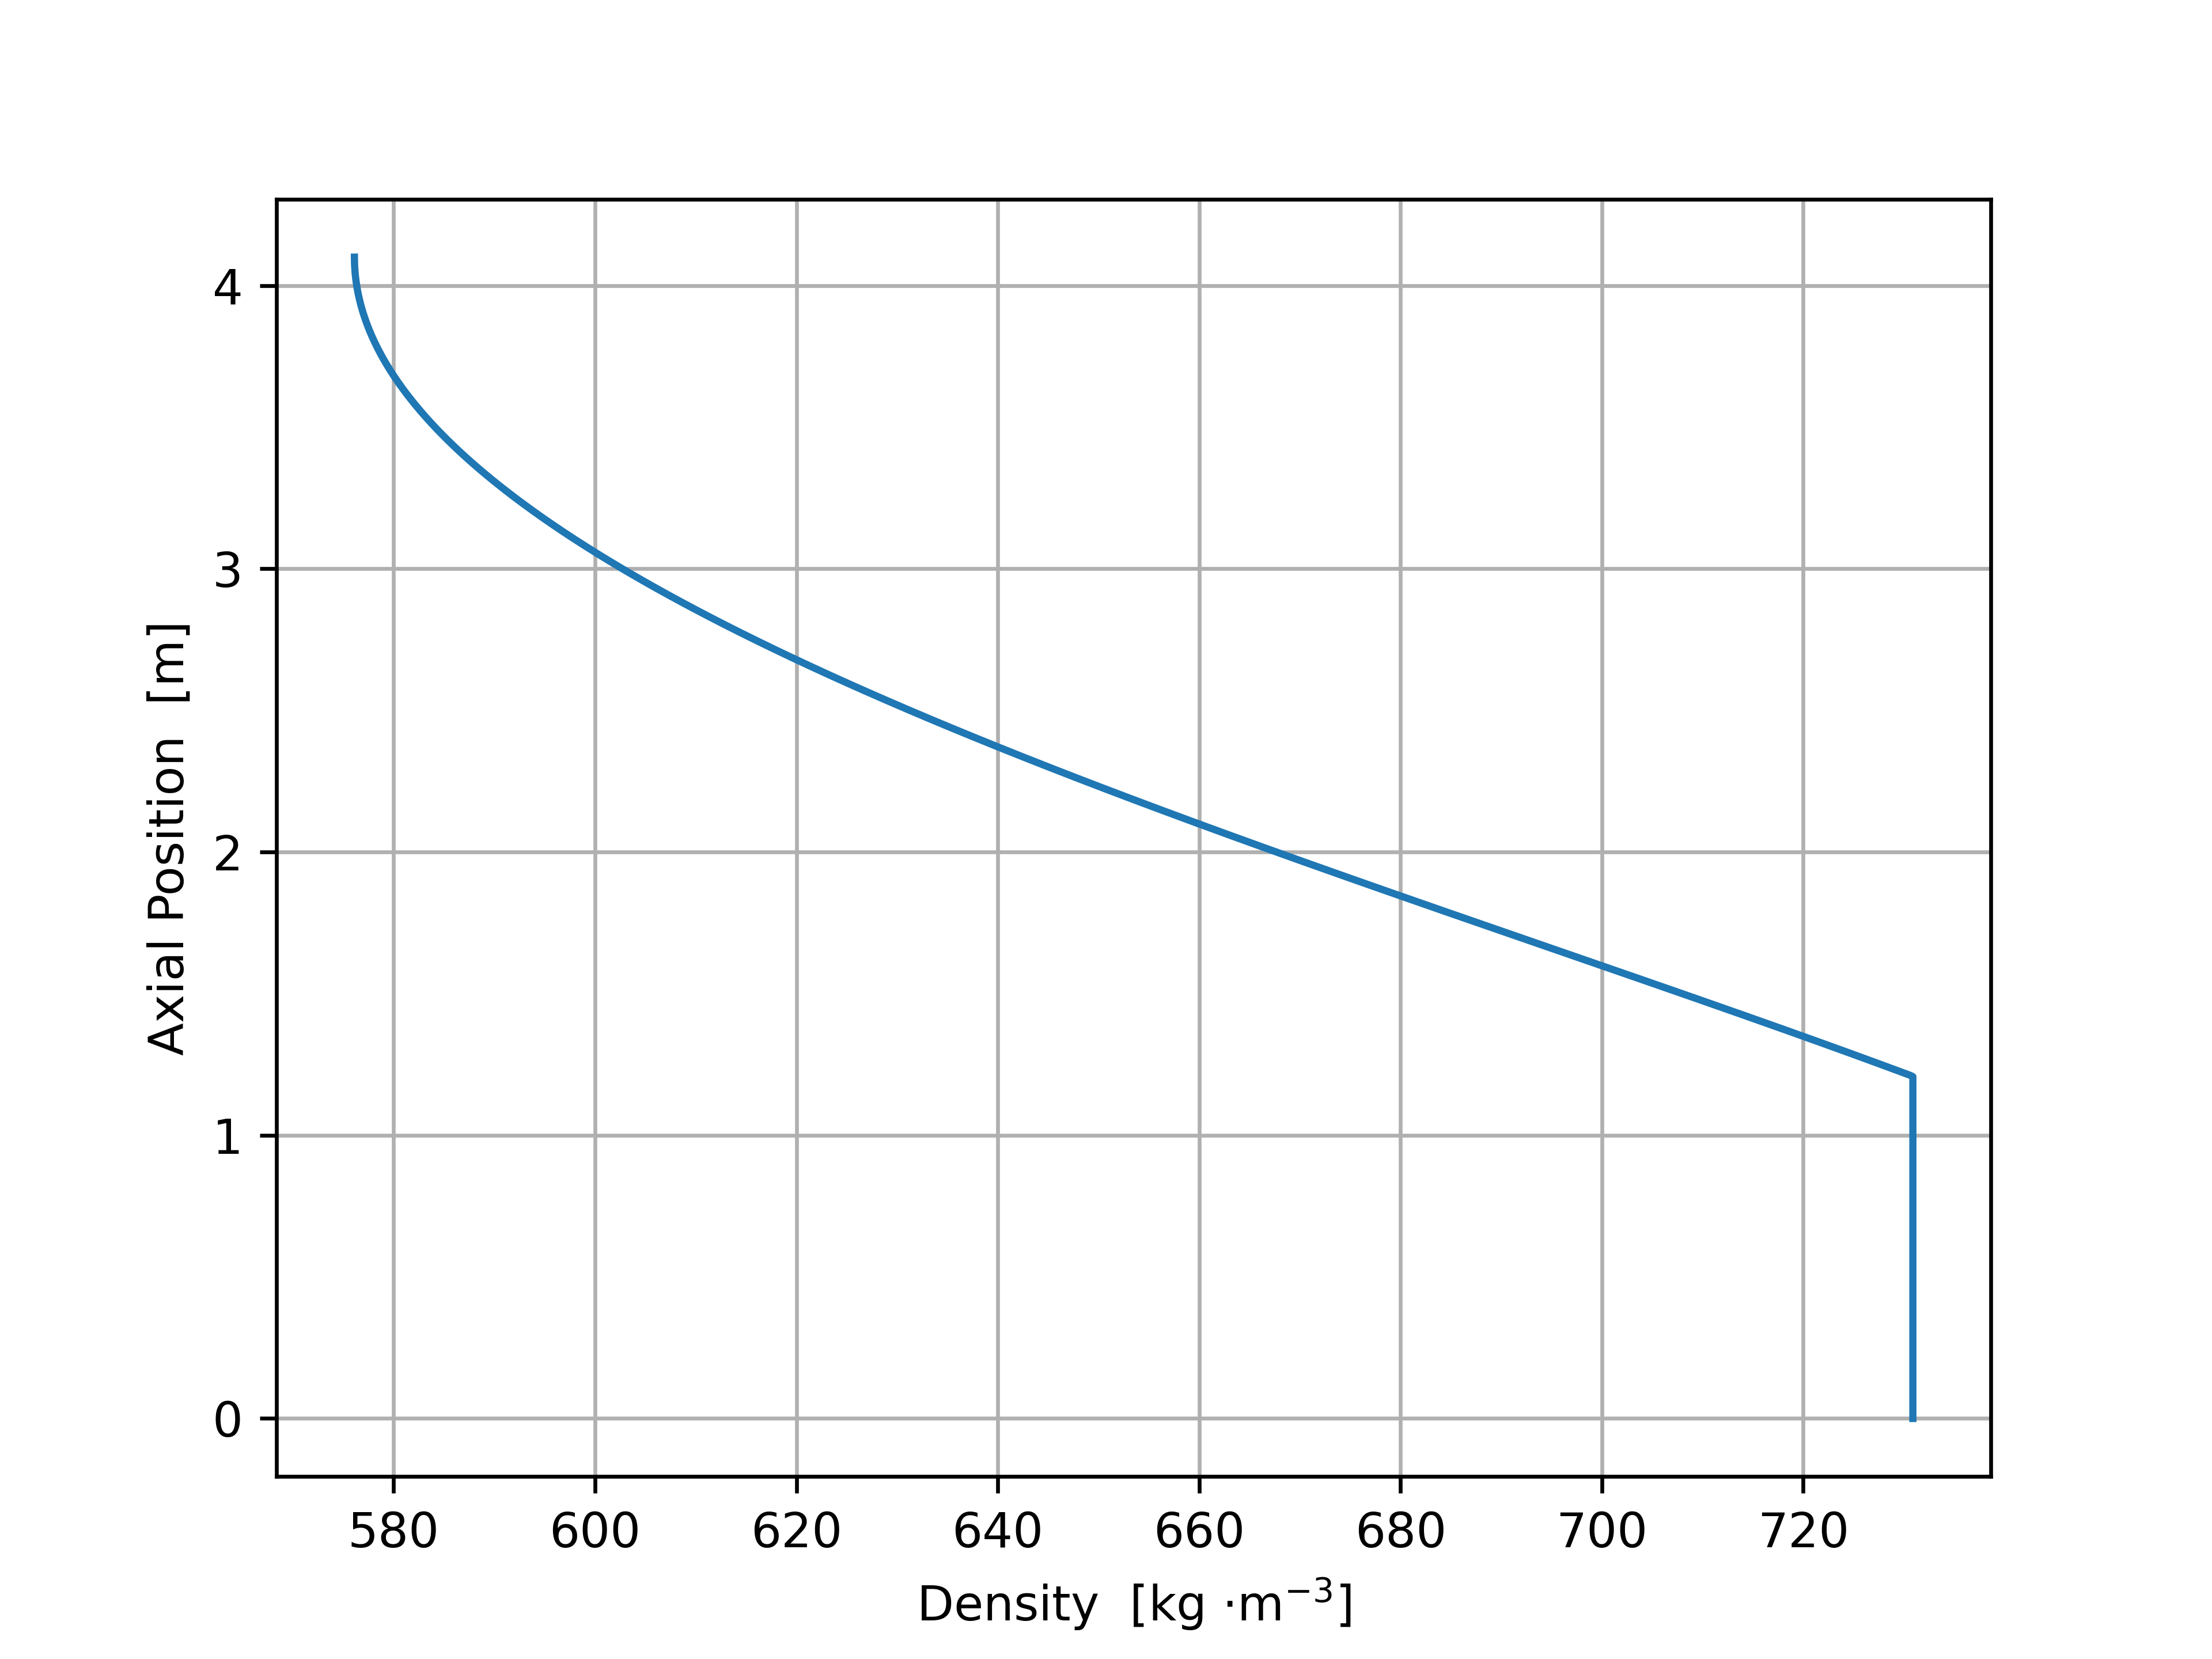
\includegraphics[width=\linewidth]{BWRplots/rho.png}
        \caption{BWR fluid density as a function of axial location}
        \label{fig:bwrdensity}
        \vspace{4ex}
    \end{minipage}
    \begin{minipage}[b]{.45\linewidth}
        \centering
        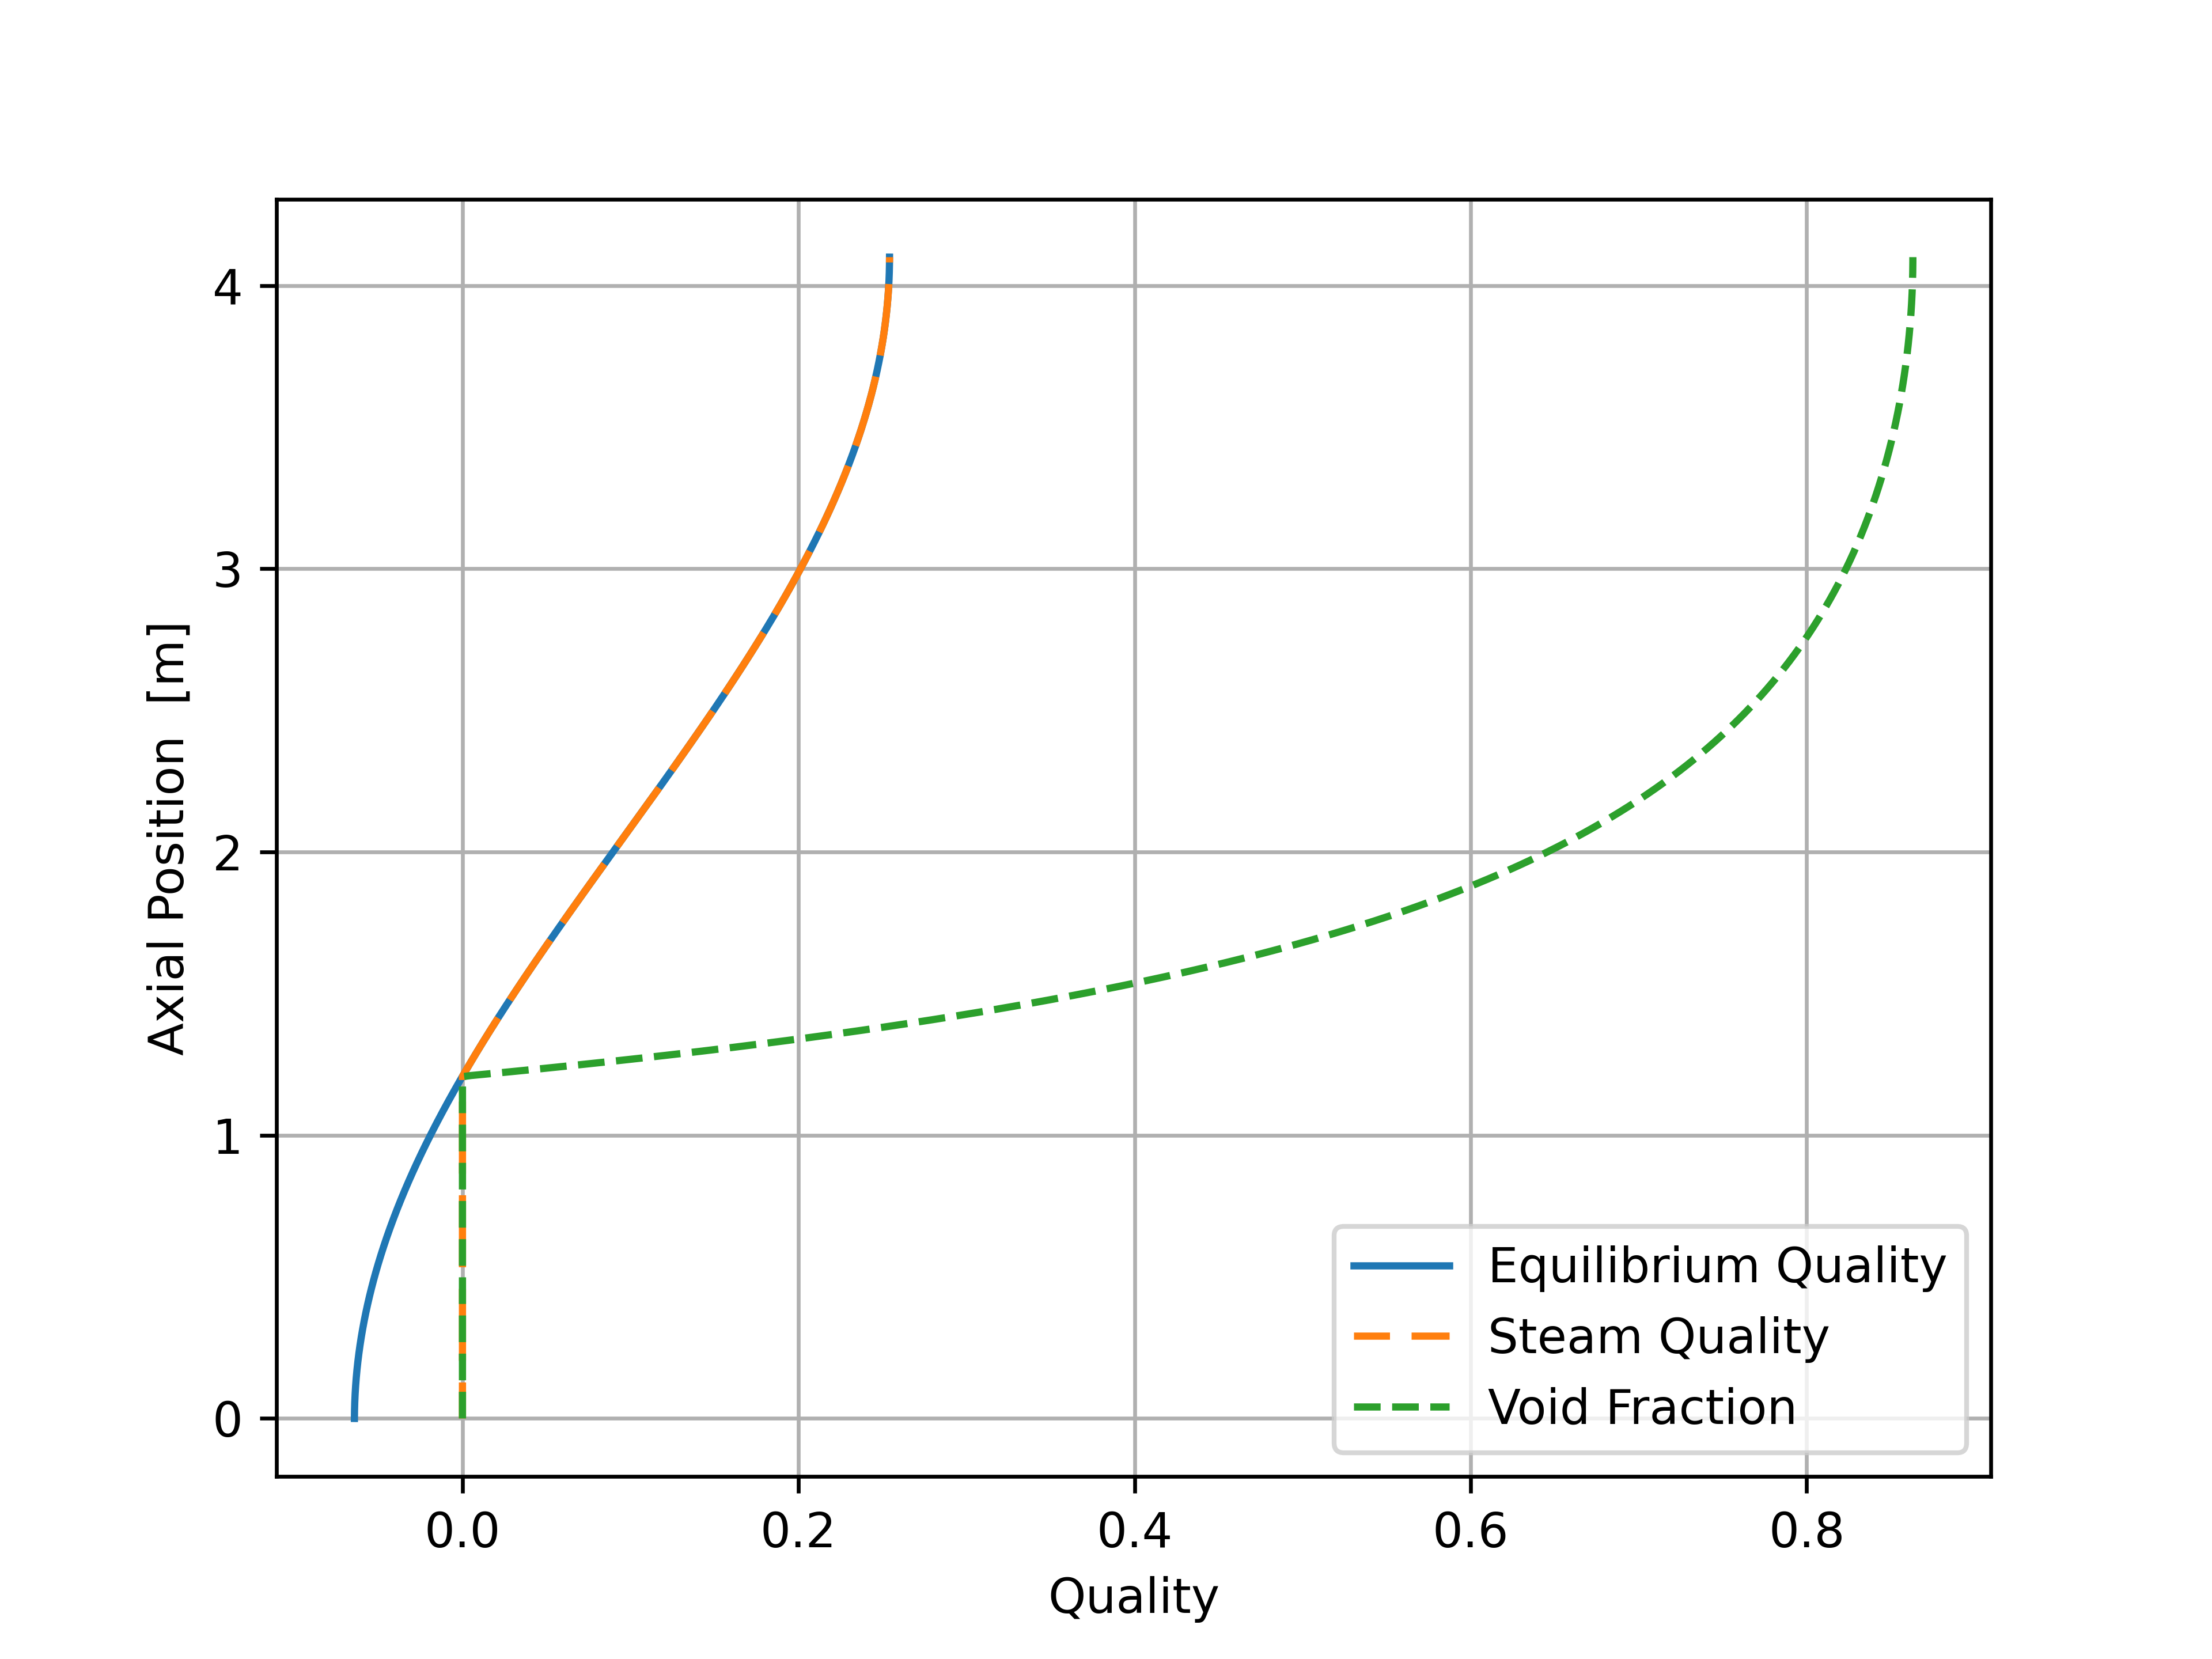
\includegraphics[width=\linewidth]{BWRplots/qualities.png}
        \caption{BWR equilibrium/steam qualities and void fraction as a function of axial location}
        \label{fig:bwrfraction}
        \vspace{4ex}
    \end{minipage}
\end{figure}

\begin{figure}[!hp!]
    \centering
    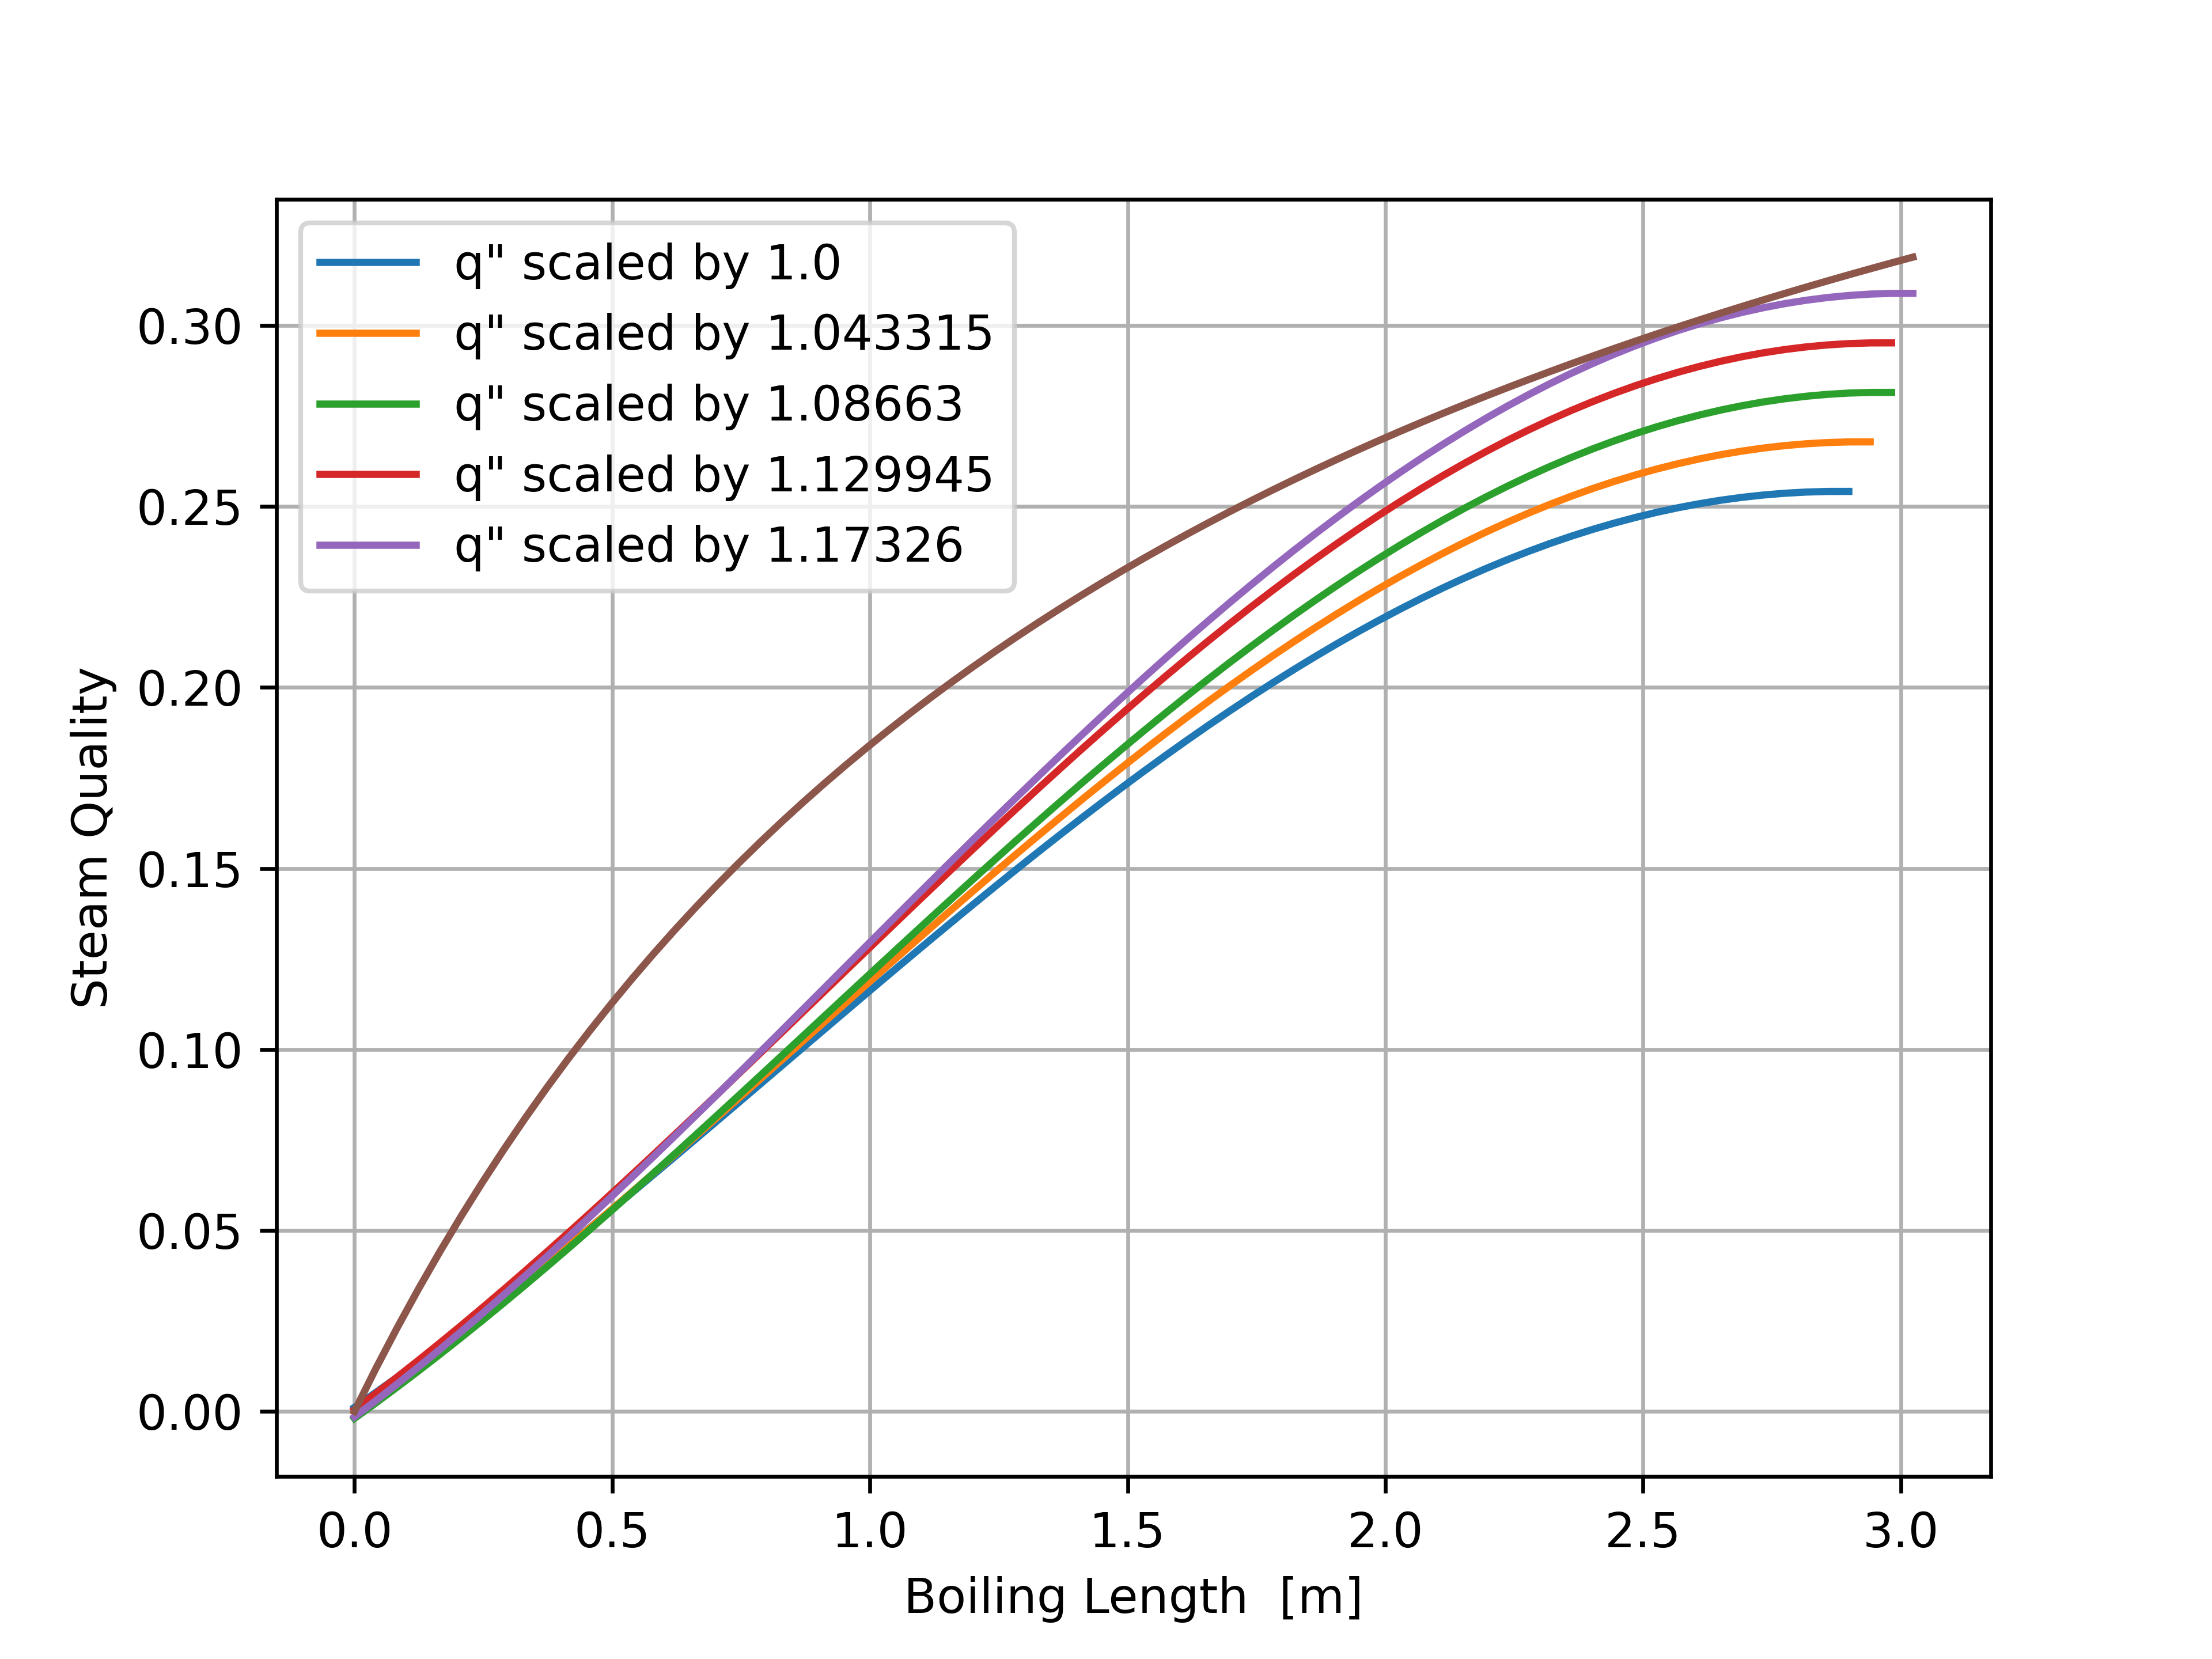
\includegraphics[width=0.5\linewidth]{BWRplots/cpr.png}
    \caption{Quality and Critical Quality as a function of boiling length}
    \label{fig:bwrcritx}
\end{figure}
\clearpage

\begin{figure}[!hp!]
    \begin{minipage}[b]{.45\linewidth}
    \centering
        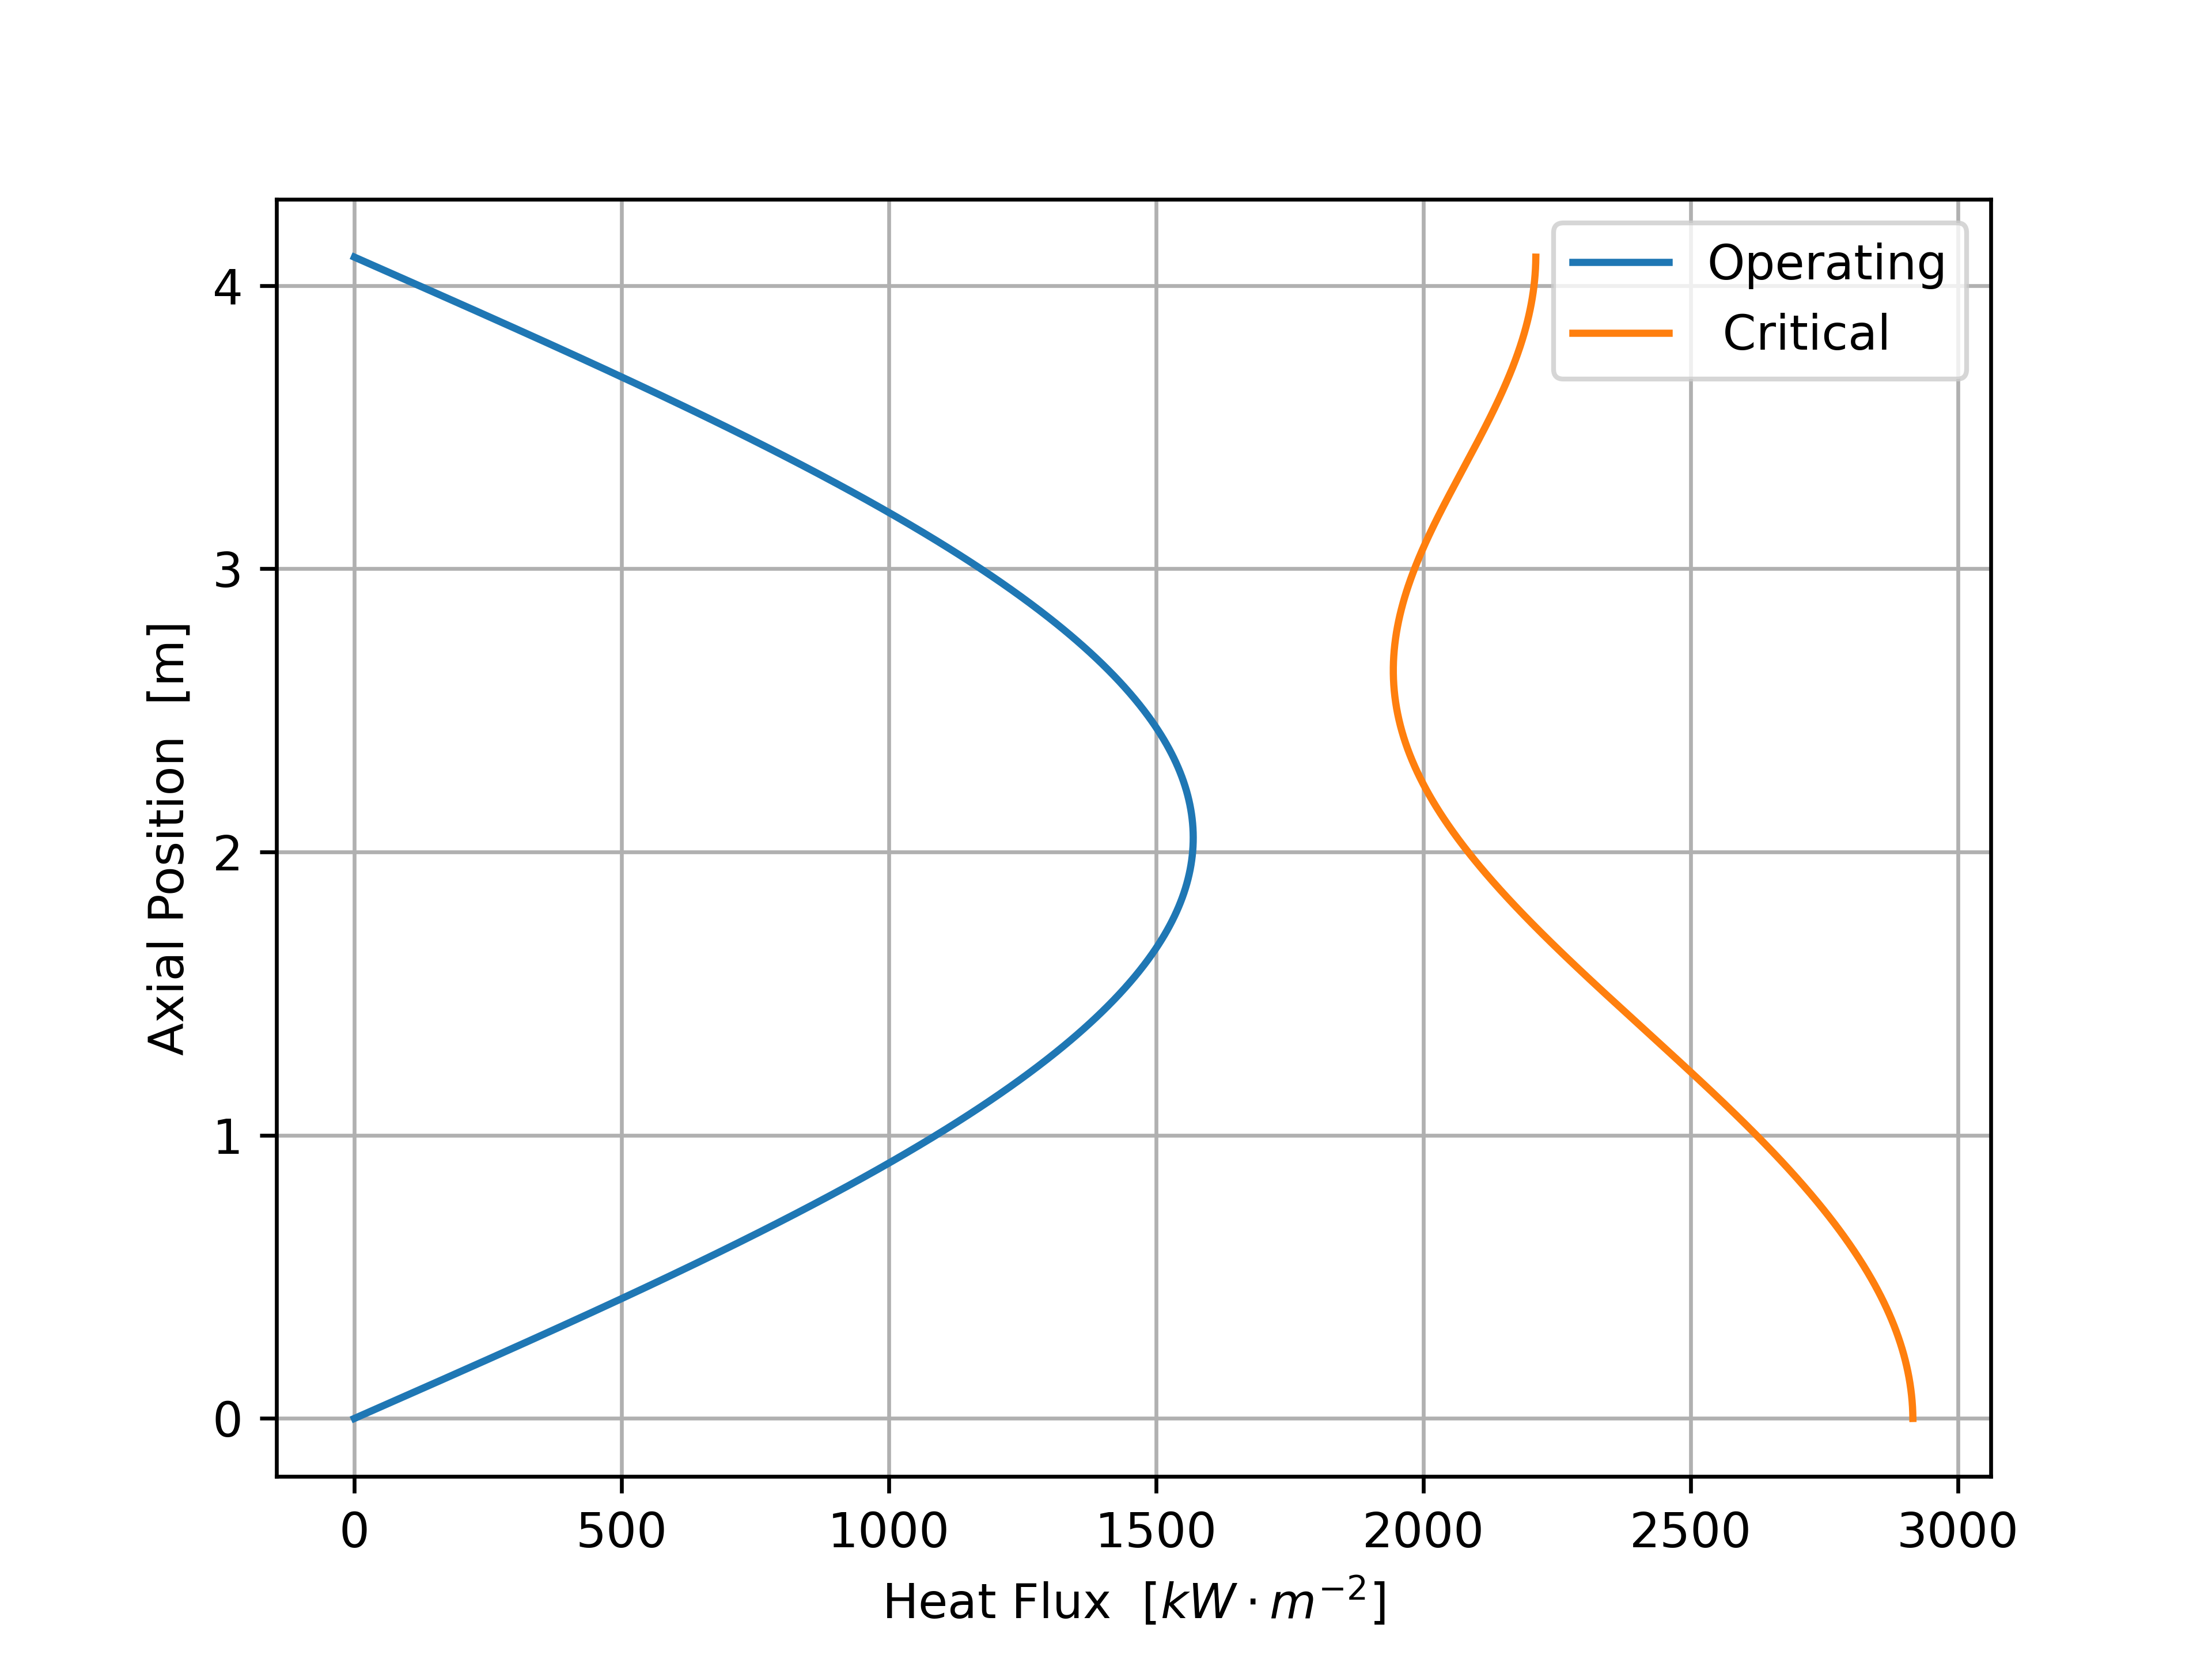
\includegraphics[width=\linewidth]{BWRplots/dnb.png}
        \caption{BWR critical and operational heat flux as functions of axial location}
        \label{fig:bwrdnb}
        \vspace{4ex}
    \end{minipage}
    \begin{minipage}[b]{.45\linewidth}
    \centering
        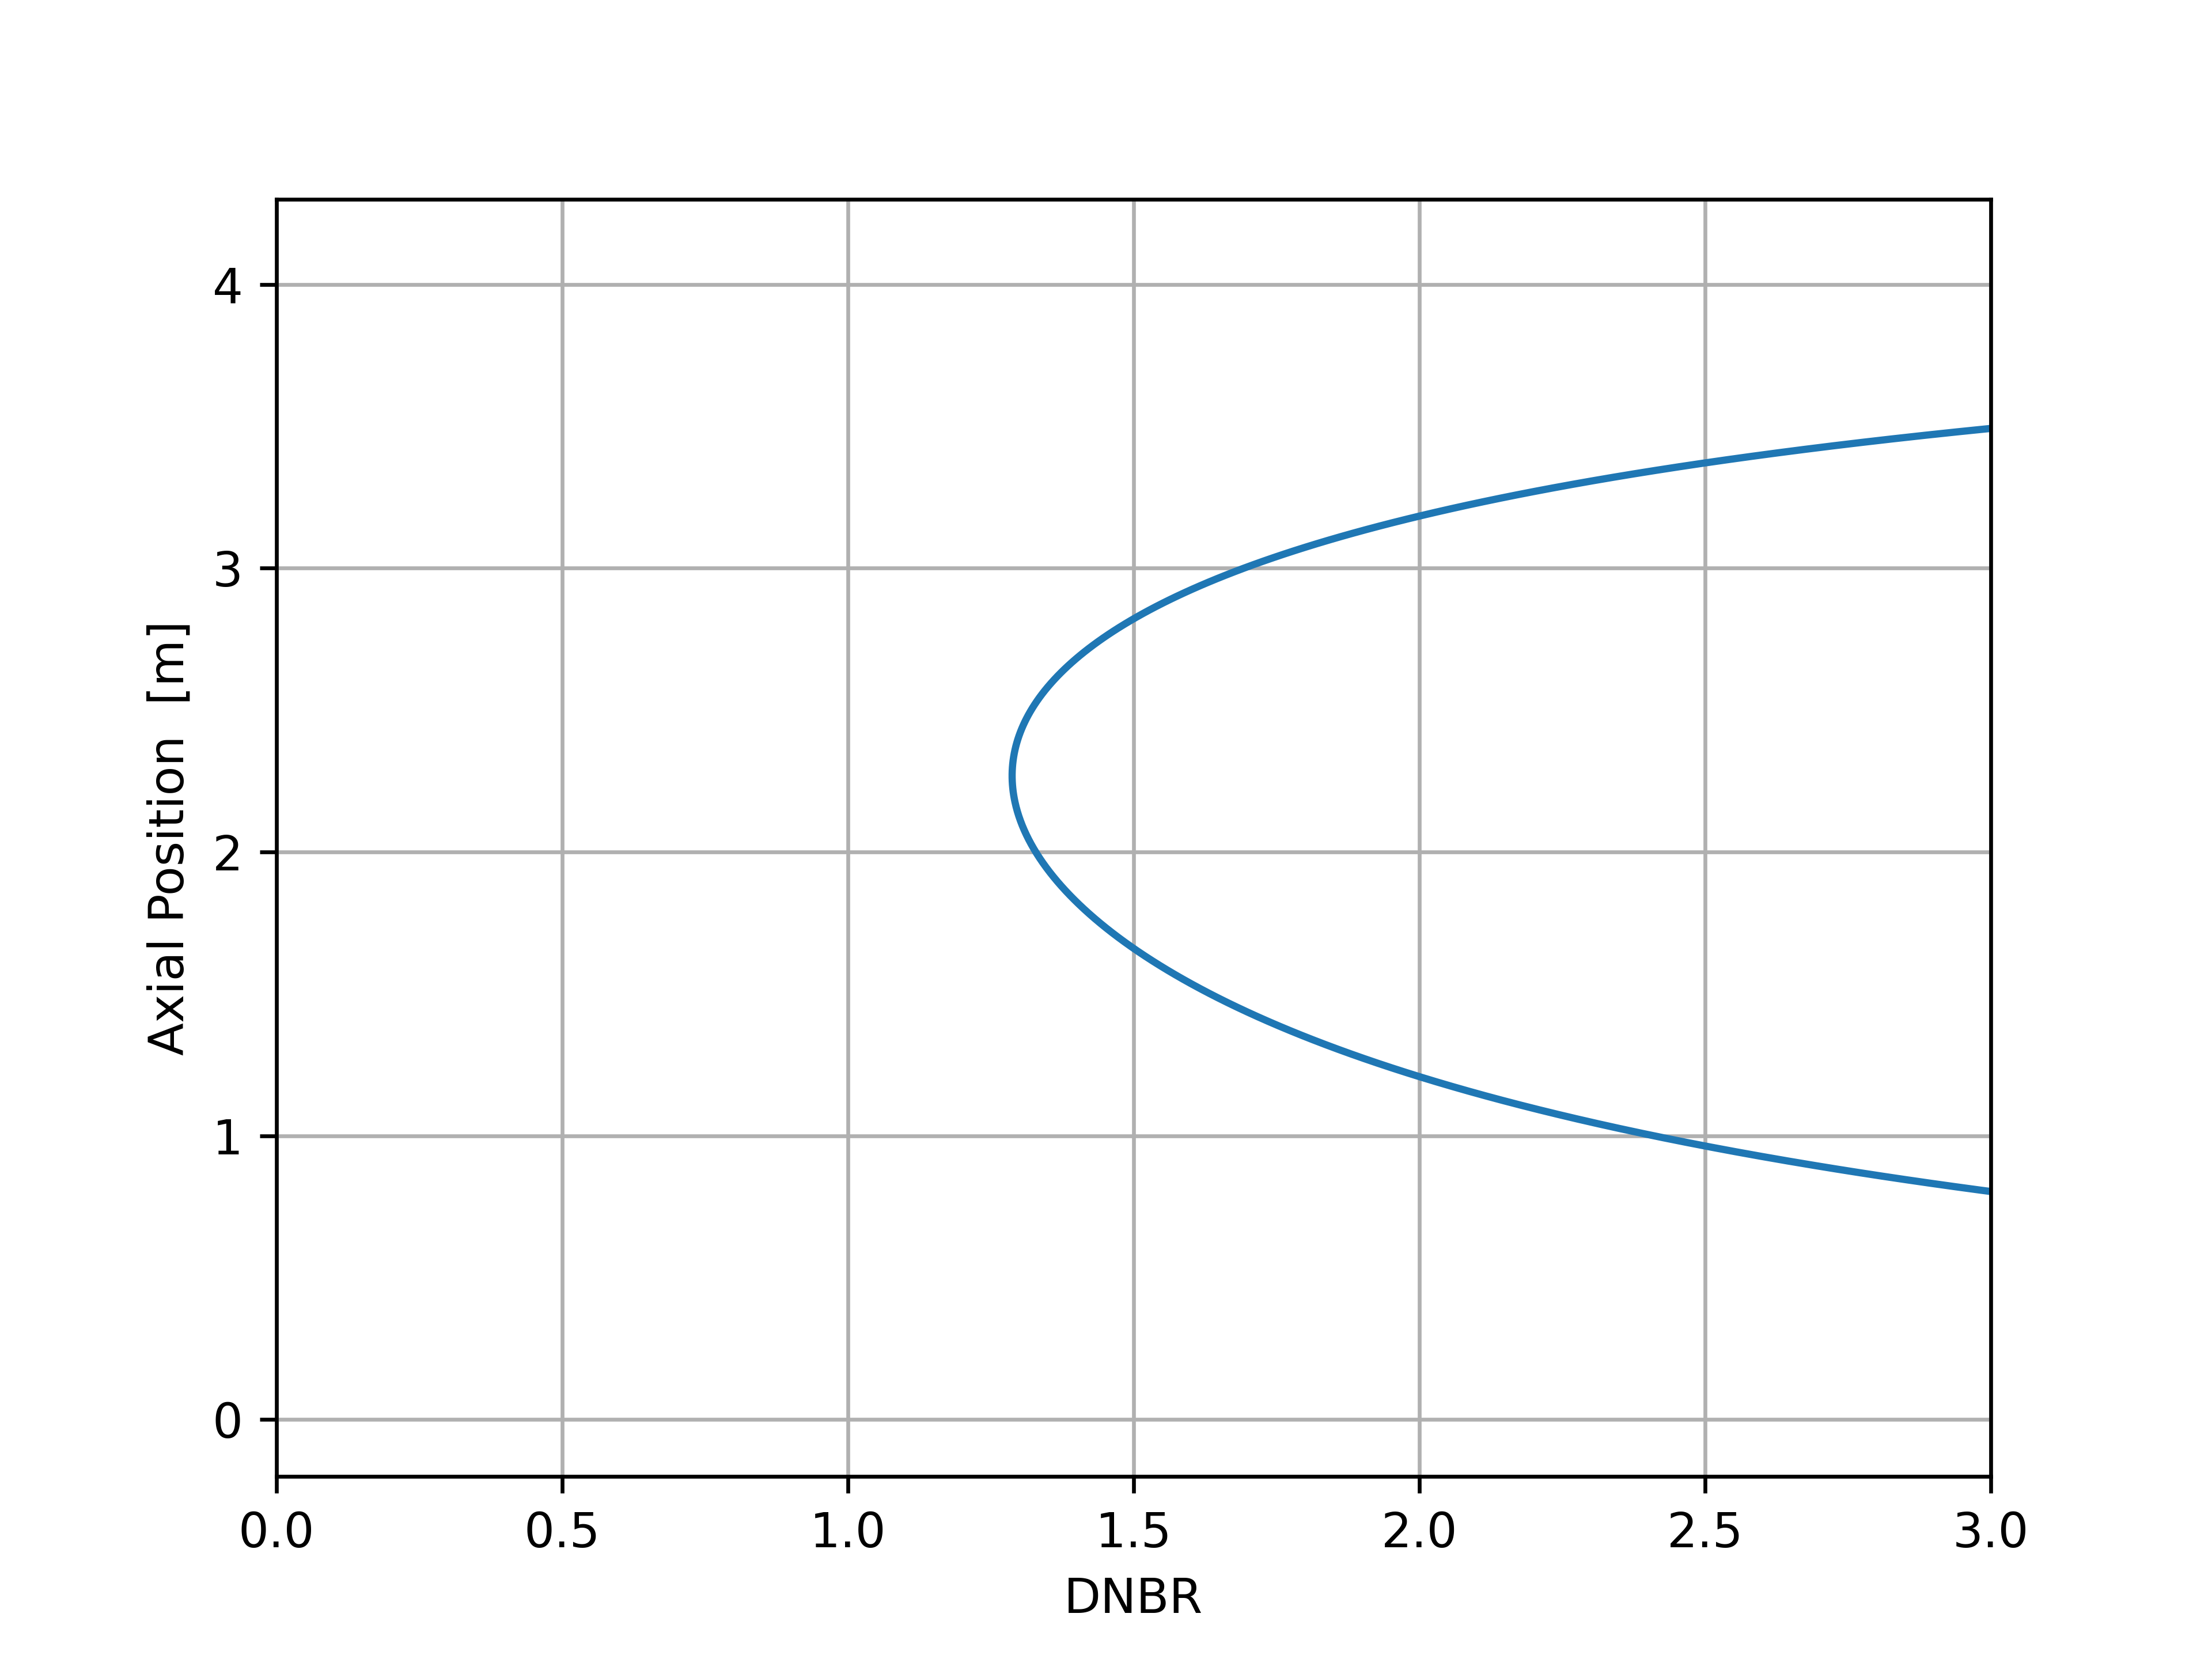
\includegraphics[width=\linewidth]{BWRplots/dnbr.png}
        \caption{BWR DNBR as a function of axial location}
        \label{fig:bwrdnbr}
        \vspace{4ex}
    \end{minipage}
\end{figure}
Finally, the sensitivity of the maximum center-line temperature to the predefined maximum linear power, mass flux, inlet fluid temperature, the inlet fluid pressure was investigated. To do this, simulations were re-run with 5 different values for each parameter, outputting only the maximum center-line temperature. These results are presented below in Table \ref{tab:bwrsens}.

\begin{table}[!hp!]
    \centering
    \renewcommand{\arraystretch}{1.5}
    \caption{Sensitivity of BWR maximum center-line temperature to select inputs}
    \label{tab:bwrsens}
    \begin{tabular}{|c|c|c|c|c|c|c|}
        \toprule
        \bottomrule
        $q'_{0}$  [$W\cdot cm^{-1}$] & 302.5 & 453.75 & 605.0 & 756.25 & 907.5 \\
        \hline
        $T_{max,CL}$  [$K$] & 1458.415 & 1903.436 & 2348.186 & 2792.779 & 3237.268 \\
        \toprule
        \bottomrule
        $G$  [$kg\cdot m^{-2} \cdot s^{-1}$] & 1175.0 & 1762.5 & 2350.0 & 2937.5 & 3525.0 \\
        \hline
        $T_{max,CL}$  [$K$] & 2348.155 & 2348.209 & 2348.186 & 2348.104 & 2347.977 \\
        \toprule
        \bottomrule
        $T_{fluid,inlet}$  [$K$] & 450.949 & 479.134 & 507.318 & 535.502 & 558.050 \\
        \hline
        $T_{max,CL} $ [$K$] & 2344.106 & 2346.634 & 2347.937 & 2348.145 & 2348.254 \\
        \toprule
        \bottomrule
        $P_{inlet}$  [$MPa$] & 5.625 & 6.5625 & 7.5 & 8.4375 & 9.375 \\
        \hline
        $T_{max,CL}$ [$K$] & 2331.805 & 2339.879 & 2348.186 & 2355.734 & 2362.664 \\
        \toprule
    \end{tabular}
\end{table}

\subsubsection{Analysis}
To begin, investigating Figure \ref{fig:bwrcoolant}, the fluid temperature reaches the saturation temperature, and then stays consistent with the saturation temperature. This is to be expected, as there is bulk boiling in a BWR, and thus while the steam quality is below 1 the fluid temperature is simply the saturation temperature. Next, investigating the clad temperature distribution, we notice some odd behavior occurring after the onset of nucleate boiling. This rapid de-acceleration of the temperature increase is due to much better heat transfer, as $2\Phi$ heat transfer is orders of magnitude stronger at transferring heat than $1\Phi$. Unfortunately, similair to the PWR scenario, the onset of nucleate boiling has little impact on the fuel temperature distributions. There are two reasons for this: gap resistance and thermal conductivity. First, the gap being present adds a large resistance to heat conduction between the fuel and clad, as seen in Figures \ref{fig:bwrh4} through \ref{fig:bwrzmax}, where the gap temperature distribution is again practically vertical. Further, the thermal conductivity of the fuel is exceedingly poor, resulting in larger temperature gradients in the fuel than ideal. Additionally, the rod diameter increased from the PWR scenario, and thus the heat has to travel further distance, and the gap thickness was nearly doubled, drastically increasing the resistance of the gap. Both of these combined result in a much higher center-line temp than observed in the PWR. To continue, the pressure drop is nearly perfectly linear, again to be expected as their are no minor losses from pipe bends or other geometry changes. The minor discrepancy from linear is explained by the rapid change in density and void fraction as the fluid traverses the channel. Further, investigating the density, void fraction, and qualities, we notice very strong differences in results. Notably, the void fraction is much higher than the quality. This is explained by quality being a mass ratio, and void fraction being a volume ratio, and vapor takes up more space per unit mass than water. Finally, the MDNBR for this BWR channel is 1.2873, lower than the thermal design criteria of 1.3, and thus this BWR is not safe with regards to the thermal design criteria for DNBR. Further, the MCPR for this BWR channel is 1.17326, again lower than the thermal design criteria for the CPR. Thus this BWR design does not meet the required thermal design criteria and is not safe to operate. 

Lastly, Investigating the sensitivity of the maximum center-line temperature on the maximal linear power, mass flux, inlet fluid temperature, and inlet pressure. First, we notice a strong correlation between the maximal linear power and the center-line temperature, to the point of increasing the linear power by a factor of only 1.5 results in fuel meltdown. This makes sense as the predominant component governing the center-line temperature is the volumetric power, which is related to the linear power by a constant (cross-sectional area of the fuel). Further, as expected when the mass flux increases  the center-line temperature decreases, albeit minimally. This minimal change is entirely due to the high thermal resistance of the gap and the thermal conductivity of the fuel, forcing poor conduction out of the fuel. However, this simulation result is not actually accurate, as an increase in the mass flux increases the rate of water being stripped from the clad surface by the flow, in turn increasing the probability of DNB, which would drastically increase the center-line temperature. Similarly, drastic changes in the inlet temperature of the fluid has minimal relative change on the maximum center-line temperature, again due to the poor fuel thermal conductivity and the gap resistance. The largest change in the center-line temperature as a result of altering an initial condition of the coolant flow was from decreasing the inlet pressure. This makes sense, as when the pressure decreases so does the saturation temperature, resulting in $2\Phi$ heat transfer and flow much sooner in the channel. 

\clearpage

\section{Conclusions}
In this report, sub-channel flow of two reactor channels was investigated: PWR and BWR. The HEM was utilized to approximate the effects of $2\Phi$ flow and heat transfer. The axial and radial temperature profiles of each pin was determined, aswell as the axial temperature and quality profiles of the coolant flow. The bulk flow through the PWR channel remained $1\Phi$ throughout, and the BWR bulk flow switched from $1\Phi$ to $2\Phi$, both as expected. The PWR was determined to be safe, operating well within the the safety margins imposed by MDNBR, 2.3973 as opposed to 1.3. On the contrary, the BWR was determined to be unsafe, and did not meet either thermal design criteria. The BWR channel had a MDNBR of 1.2873 as opposed to the required 1.3, and a MCPR of 1.17326 as opposed to the required 1.2. Finally, for both the PWR and BWR channels, the center-line temperature was most sensitive to the maximum linear power, and minimally sensitive to coolant flow conditions. The most impactful coolant flow condition on the center-line temperature for the PWR and BWR was the inlet temperature and the inlet pressure, respectively. 

\section{References}
\printbibliography[heading=none]

\clearpage
\section{Code Appendix}
\subsection{Execute Instructions}

There are two ways to execute the code for this report. The first is simply copy, paste, execute, and the second is a little bit harder but much, much less cluttered. 

The first way is to simply copy/paste the code in the next section into a single cell in a .ipynb file, and run the cell.

However, I recommend the following procedure, as there will be much less code to skip through to see the plots and output. To execute the code in the next section, please copy the code (excluding the final line) into a .py file, and remember where in your computer it is. With the file downloaded, a brief explanation of the code will no be presented. This code has 5 class objects, three for material properties and initial conditions, one for solving, and one for plotting. The three material property and initial condition classes are not meant to be interacted with. The solving class, called 'Solver', is the workhorse solver of the code, which actually solves for the temperature distributions and equilibrium quality. The plotting class, called 'Plotter', is the object I call to generate all relevant plots for that scenario. To use either, you must first import the .py file. This is done like so, assuming the .py file is named 'NPRE449CP.py:

\begin{python}
    import sys
    sys.path.append('path/to/.pyfile/') #path to the directory in your computer housing the .py file
    from NPRE449CP.py import *
\end{python}

now, with everything imported, to run the solver you simply run:

\begin{python}
    solver = Solver('PWR') # or 'BWR'
    solver.solveFluid(output=True) #put to false if you do not want the result at each node 
    solver.solvePinTemperature()
\end{python}

and to run the plotter (which does not need to have a solver run before it), run:

\begin{python}
    Plotter('PWR', show= True) # or 'BWR', True to show plots, False to close plots and only save
\end{python}

\clearpage
\subsection{Code}
\begin{python}
import numpy as np
from numpy.linalg import norm as norm
import scipy as scp
import matplotlib.pyplot as plt
from pyXSteam.XSteam import XSteam
np.set_printoptions(precision=3,suppress= True)
import warnings
warnings.filterwarnings("ignore") #ignore divide by zero in alpha

'''CHANGE THIS PARAMETER'''
option = 'PWR' # 'PWR' or 'BWR'
'''^^^^^^^^^^^^^^^^^^^^^'''
'''^^^^^^^^^^^^^^^^^^^^^'''
'''^^^^^^^^^^^^^^^^^^^^^'''
'''^^^^^^^^^^^^^^^^^^^^^'''

class Conditions:
    
    def __init__(self,which = 'PWR'):
        
        self.g = 9.81 # m/s2
        
        if which == 'PWR':
            self.G = 4000 #kg/m2 s
            self.qp0 = 430e2 #W/cm to W/m
            self.P0 = 15e6 #MPa to pa
            self.Tf0c = 277 #oC
        
        else:
            self.G = 2350 #kg/m2 s
            self.qp0 = 605e2 #W/cm to W/m
            self.P0 = 7.5e6 #MPa to pa
            self.Tf0c = 272 #oC
            
        self.Tf0 = self.Tf0c + 273.15

class PinProperties:
    
    def __init__(self,Conditions,which = 'PWR'):
    
        if which == 'PWR':
            
            self.H = 4 #m
            self.Drod = 0.95e-2 # cm to m 
            self.Pitch = 1.26e-2 # cm to m
            self.DFuel = 0.82e-2 # cm to m
            self.Gap_thickness = 0.006e-2 #cm to m
            self.kgap=0.25 #W/mK
            self.k_fuel=3.6 #W/mK
            self.k_cladding=21.5 #W/mK
            #self.mu = 97.575e-6
            self.muL = lambda a: 69.403e-6
            self.muV = lambda a: 22.716e-6
        
        else:
            
            self.H = 4.1 #m
            self.Drod = 1.227e-2 # cm to m
            self.Pitch = 1.62e-2 # cm to m 
            self.DFuel = 1.04e-2 # cm to m 
            self.Gap_thickness = 0.010e-2 # cm to m
            self.kgap=0.25 #W/mK
            self.k_fuel=3.6 #W/mK
            self.k_cladding=21.5 #W/mK
            #self.mu = 97.352e-6
            self.muL = lambda a: 89.451e-6
            self.muV = lambda a: 11.656e-6

        
        self.xih = self.Drod * np.pi #m
        self.SAf = self.DFuel *np.pi * self.H
        self.SAc = (self.DFuel + self.Gap_thickness) * np.pi * self.H
        self.Axsf = self.DFuel ** 2 / 4 * np.pi
        self.Rf = self.DFuel/2
        self.Rci = self.Rf + self.Gap_thickness/2
        self.Rco = self.Drod / 2 
        self.qp = lambda z: Conditions.qp0* np.sin(np.pi * z / self.H) #W/m
        self.qpp = lambda z: self.qp(z) / self.xih # w /m2
        self.q3p = lambda z: self.qp(z) / self.Axsf
        
        return

class FluidProperties:
    
    def __init__(self,ICs,Pin,poly_order=15):
        
        '''
        Steam Table
        -----------
        '''
        props = XSteam(XSteam.UNIT_SYSTEM_BARE)
        
        '''
        Constant Material Properties 
        ----------------------------
        '''
        _p0,_tf0 = ICs.P0/1e6,ICs.Tf0 # Initial Pressure [MPa] and Temp [K]
        self.cp = props.Cp_pt(_p0,_tf0) * 1e3 #kj/kg -> j/kg
        self.mu = props.my_pt(_p0,_tf0)  # N s / m2
        self.k = props.tc_pt(_p0,_tf0)  # W/ m K

        '''
        Pressure Variant Properties
        ---------------------------
        '''
        self.hg = lambda P: props.hV_p(P) * 1e3 # kJ/kg -> j/kg
        self.hf = lambda P: props.hL_p(P) * 1e3 # kJ/kg -> j/kg
        self.hfg = lambda P: self.hg(P) - self.hf(P)
        self.tsat = lambda P: props.tsat_p(P) # K

        '''
        Initial Properties
        ------------------
        '''
        self.X_e0 = self.cp*(_tf0 - self.tsat(_p0))/self.hfg(_p0)
        self.rho0 = props.rho_pt(_p0,_tf0) #kg /m3

        '''
        Pipe Dimensions
        ---------------
        '''
        self.Area = (Pin.Pitch**2 - 1/4 * np.pi * Pin.Drod**2) #m2
        self.xiw = Pin.xih #m
        self.Dh = 4 * self.Area / (self.xiw) #m
        
        '''
        Dimensionless Groups
        ----------------------
        '''
        self.Re = lambda Xe, P: ICs.G * self.Dh / self.mu#m(Xe,P)
        self.Pr = lambda Xe, P: self.cp * self.mu / self.k
        self.Nu = lambda Xe, P: 0.023 * self.Re(Xe, P)**(.8) * self.Pr(Xe, P) ** (0.4)
        self.h = lambda Xe, P: self.Nu(Xe, P) * self.k / self.Dh 
        self.__f = lambda Xe, P: self.Re(Xe, P) ** (-.25) * 0.316

        '''
        Two-Phase Properties
        --------------------
        '''
        self.rhosatratio = lambda P: props.rhoV_p(P) / props.rhoL_p(P)
        self.alpha = lambda Xe: 1 / (1 + (Xe**(-1) - 1) * self.rhosatratio(_p0))
        self.rhofg = props.rhoL_p(_p0) - props.rhoV_p(_p0)
        self.vgf = -1/props.rhoL_p(_p0) + 1/props.rhoV_p(_p0)
        self.rhoL = props.rhoL_p(_p0)
        self.rhoV = props.rhoV_p(_p0)
        self.rhom = lambda Xe, P: self.rhoL if Xe<0 else (1/self.rhoL + 1/self.rhofg*Xe)**(-1)
            #for props.my_pt, for whatever reason pyXSteam doesnt have mu at saturation
            #so you have to alter tsat a littlebit
        self.mum = lambda Xe, P: Pin.muL(P) if Xe <0 else (Xe / Pin.muV(P) + (1 - Xe)/Pin.muL(P))**(-1)
        self.f = lambda Xe, P: self.__f(Xe,P) if Xe < 0 else 0.046 * self.Re(Xe,P)**(-0.2) * (self.mum(Xe, P) / Pin.muL(P)) **(0.2)


        '''
        Material Property Fits
        ----------------------
        '''
        self.__pressures = np.linspace(1,20,1000)
        self.__hf_data = [self.hf(P) for P in self.__pressures] 
        self.__hg_data = [self.hg(P) for P in self.__pressures]

        #fitting with 15th order polynomial with numpy.polyfit and np.polynomial.Polynomials
        #polyfit returns high -> low, polynomial.Polynomial takes low -> high 
        #only setting as object for plotting
        self.__hf_fit = np.polynomial.Polynomial( np.flip( np.polyfit(self.__pressures*1e6,self.__hf_data,poly_order) ) ) 
        self.__hg_fit = np.polynomial.Polynomial( np.flip( np.polyfit(self.__pressures*1e6,self.__hg_data,poly_order) ) ) 

        self.dhfdp = self.__hf_fit.deriv()
        self.dhgdp = self.__hg_fit.deriv()
        
        return

    def plot(self):
        
        p,hfdata,hgdata = self.__pressures, self.__hf_data, self.__hg_data
        hf_fit = self.__hf_fit(p*1e6)
        hg_fit = self.__hg_fit(p*1e6)

        hf_norm = norm(hf_fit - hfdata,2) / norm(hfdata,2)
        hg_norm = norm(hg_fit - hgdata,2) / norm(hgdata,2)
        
        fig,ax = plt.subplot_mosaic([['h_f','h_g']],figsize = (12,5),gridspec_kw={'wspace':.2})
        
        ax['h_f'].plot(p, hfdata, label = 'pyXSteam Data')
        ax['h_f'].plot(p, hf_fit, label = 'h$_f$ Polynomial Fit')
        ax['h_f'].set_ylabel('h$_f$  [J $\cdot$ kg$^{-1}$]')

        ax['h_g'].plot(p, hgdata, label = 'pyXSteam Data')
        ax['h_g'].plot(p, hg_fit, label= 'h$_{g}$ Polynomial Fit')
        ax['h_g'].set_ylabel('h$_{g}$  [J $\cdot$ kg$^{-1}$]')

        for plot in ax:
            ax[plot].set_xlabel('Pressure  [MPa]')
            ax[plot].grid()
            ax[plot].legend()

        print(f'hf Fit L2 Norm: {hf_norm}\nhg Fit L2 Norm: {hg_norm}')
        
        
        return 
        
'''
SOLVER
'''
class Solver:
    
    def __init__(self,which = 'PWR',num_zsteps = 100,param=None,val=None):
        try:
            assert(which in ['PWR','BWR'])
        except AssertionError:
            errormessage = f"The reactor type '{which}' is not supported. Valid reactor types are: 'BWR' or 'PWR'"
            raise Exception(errormessage)
        self.which = which
        self.ICs = Conditions(which=which)
        if param != None:
            self.ICs.__dict__[param] = val
        self.pin = PinProperties(which=which,Conditions=self.ICs)
        self.fluid = FluidProperties(self.ICs,self.pin)
        self.z = np.linspace(0,self.pin.H,num_zsteps)
        
        return


    def solveFluid(self,output = True):
        
        ICs,pin, fluid = self.ICs, self.pin, self.fluid
        z = self.z
        P = [ICs.P0]
        X_e = [fluid.X_e0]
        T_f = [ICs.Tf0]
        if output:
            print('Z-Coordinate\tPressure\tSteam Quality\tFluid Temperature')
            print('-----------------------------------------------------------------')
            print(f'{np.trunc(z[0],)}\t\t{np.around(P[0]*1e-6,3)}\t\t{np.around(X_e[0],4)}\t\t{np.around(T_f[0],3)}')
        for i in range(1, len(z)):
            
            dz = z[i]- z[i-1]
            
            '''
            Solving for Pressure
            Solve for pressure using the material properties at the previous z
            '''
            rhom = fluid.rhom(X_e[i-1],P[i-1]*1e-6)
            f = fluid.f(X_e[i-1],P[i-1]*1e-6)
            topP1 = 1/2 * fluid.xiw / fluid.Area * f * ICs.G**2 / rhom
            topP2 = rhom * ICs.g
            topP3 = ICs.G * pin.qp(z[i]) * fluid.vgf/ ( fluid.Area * fluid.hfg(P[i-1]*1e-6))
            botP1 =  fluid.dhfdp(P[i-1]) if X_e[i-1] < 0 else X_e[i-1] * fluid.dhgdp(P[i-1]) + (1-X_e[i-1]) * fluid.dhfdp(P[i-1])
            botP2 = 1 - ICs.G**2 * fluid.vgf/ (fluid.hfg(P[i-1]*1e-6)) * botP1
            insideP = (topP1 + topP2 + topP3) / botP2
            P_i = P[i-1] - dz *insideP

            '''
            Solving for Steam Quality
            Solve for steam quality using current pressure
            '''
            dpdz = (P_i - P[i-1]) / dz
            insideXe1 = fluid.dhfdp(P_i) * dpdz if X_e[i-1] < 0 else X_e[i-1] * fluid.dhgdp(P_i) * dpdz + (1 - X_e[i-1]) * fluid.dhfdp(P_i) * dpdz
            insideXe2 = pin.qp(z[i]) / (fluid.Area * ICs.G * fluid.hfg(P_i* 1e-6)) - 1/fluid.hfg(P_i * 1e-6) * insideXe1
            X_e_i = dz * insideXe2 + X_e[i-1]

            '''
            Solving for Temperature
            Find temperature with current properties
            '''
            T_f_i = fluid.hfg(P_i*1e-6) / fluid.cp * X_e_i + fluid.tsat(P_i*1e-6) if X_e_i < 0 else fluid.tsat(P_i*1e-6)

            '''
            Printing
            '''
            if output:
                print(f'{np.around(z[i],3)}\t\t{np.around(P_i*1e-6,3)}\t\t{np.around(X_e_i,4)}\t\t{np.around(T_f_i,3)}')
            
            '''
            Appending Pressure, Steam Quality, and Fluid Temperature lists
            lists are better than numpy arrays for on the fly changing...
            '''
            P.append(P_i)
            X_e.append(X_e_i)
            T_f.append(T_f_i)
            
        
        self.PFunc = scp.interpolate.interp1d(z,np.array(P)*1e-6)
        self.XeFunc = scp.interpolate.interp1d(z,X_e)
        self.TFluidFunc = scp.interpolate.interp1d(z,T_f)
        
        return


    def __solveCladSurface(self):

        ICs, pin, fluid = self.ICs, self.pin, self.fluid

        Pc = 22.064
        M = 18.01528
        F = lambda Xe,P: 1 if Xe < 0 else (1 + Xe * fluid.Pr(Xe,P) * (fluid.rhosatratio(P) - 1)) ** (0.35)
        S = lambda Xe,z: (1 + 0.055 * F(Xe,self.PFunc(z)) ** (0.1) * (fluid.Re(Xe, self.PFunc(z)))**(0.16)) ** (-1)
        hnb = lambda z: 55 * (self.PFunc(z) / Pc) ** (0.12) * pin.qpp(z)**(2/3) * (-np.log10(self.PFunc(z)/Pc))**(-0.55) * M**(-0.5)
        def twophase(Tw,z,Xe):
            P = self.PFunc(z)
            fpart = (F(Xe,P) * fluid.h(Xe, P) * (Tw - self.TFluidFunc(z)))**2
            spart = (S(Xe,z) * hnb(z) *(Tw - fluid.tsat(self.PFunc(z))))**2
            return pin.qpp(z) - (fpart + spart) **(.5)
        def onephase(z,Xe):
            P = self.PFunc(z)
            return pin.qpp(z) / fluid.h(Xe,P) + self.TFluidFunc(z)

        T_cs = []
        guess = fluid.tsat(ICs.P0/1e6) #* 1.5
        for i,z in enumerate(self.z):
            X_e_i = self.XeFunc(z)
            tempGuess = onephase(z, X_e_i)
            if tempGuess < fluid.tsat(self.PFunc(z)):
                T_cs.append(tempGuess)
            else:
                try:
                    _ = self.ONB * 3
                except:
                    self.ONB = z
                func = lambda Tw: twophase(Tw,z,X_e_i)
                root = scp.optimize.root(func,guess).x[0]
                T_cs.append(root)

        try:
            self.SatBoil = scp.optimize.root(self.XeFunc, pin.H/3).x[0]
        except ValueError:
            pass
        self.TCladS = scp.interpolate.interp1d(self.z,T_cs)
        return
            

    def solvePinTemperature(self):

        self.__solveCladSurface()
        ICs,pin, fluid = self.ICs, self.pin, self.fluid

        C3 = lambda z: -pin.q3p(z)*pin.Rf**2 / 2 / pin.kgap #yes
        C5 = lambda z: pin.kgap / pin.k_cladding * C3(z) 
        C6 = lambda z: self.TCladS(z) - C5(z)*np.log(pin.Rco)
        C4 = lambda z: C5(z)* np.log(pin.Rci) - C3(z)* np.log(pin.Rci) + C6(z)
        C2 = lambda z: pin.q3p(z) * pin.Rf**2 / 4 / pin.k_fuel + C3(z) * np.log(pin.Rf) + C4(z)

        self.TFuelFunc = lambda r, z: -pin.q3p(z) * r**2 / 4 / pin.k_fuel + C2(z)
        self.TGapFunc = lambda r, z: C3(z) * np.log(r) + C4(z)
        self.TCladFunc = lambda r, z: C5(z) * np.log(r) + C6(z)
        
        return
        

class Plotter:
    
    def __init__(self, which = 'PWR', ideal_steps = 1000, show = False):

        self.zsteps = ideal_steps
        solver = Solver(which=which,num_zsteps=self.zsteps)
        solver.solveFluid(output=False)
        solver.solvePinTemperature()
        self.solution = solver
        self.savepath = which + 'plots/'
        try:
            assert(which in ['PWR','BWR'])
        except AssertionError:
            errormessage = f"The reactor type '{which}' is not supported. Valid reactor types are: 'BWR' or 'PWR'"
            raise Exception(errormessage)
        self.__MESH(which,show)
        self.__BOTH(show)
        if which == 'BWR':
            self.__BWR(show)
        self.__SENSITIVITY(which)
        return
    def __finisher(self, ax, xlabel='t',legend=0,loc=None):
        xlabel = 'Temperature  [K]' if xlabel == 't' else 'Pressure  [MPa]'
        ax.grid()
        if legend:
            ax.legend(loc = loc)
        ax.set_xlabel(xlabel)
        ax.set_ylabel('Axial Position  [m]')
    def __radfinisher(self, ax):
        ax.grid()
        ax.legend()
        ax.set_xlabel('Radial Position  [m]')
        ax.set_ylabel('Temperature  [K]')

    
    def __show(self,show,name):
        plt.savefig(self.savepath+name+'.png', dpi=600)
        if show:
            plt.show()
        else:
            plt.close()
        
    @staticmethod   
    def __latex(arr, name):
        component = f'{name} & '
        maxcl = 'T_{max,CL}  [$K$] & '
        for comp, tcl in arr:
            component += str(comp) + ' & '
            maxcl += str(np.around(tcl,3)) + ' & '

        print('\\toprule\n\\bottomrule')
        print(component[:-2]+'\\\\')
        print('\hline')
        print(maxcl[:-2]+'\\\\')
        
        return


    def __MESH(self, which,show =False):
        fig, ax = plt.subplots()
        for n in [2,3,5,10,100, 1000]:
            solve = Solver(which,n)
            solve.solveFluid(output=False)
            ax.plot(solve.TFluidFunc(solve.z), solve.z, label = f'{n} Nodes')
        self.__finisher(ax,legend=1)
        self.__show(show,'mesh')
        return

    def __BOTH(self, show = False):

        solution = self.solution
        z = solution.z

        TFluid = solution.TFluidFunc(z)
        TCladSO = solution.TCladS(z)
        TCladSI = solution.TCladFunc(solution.pin.Rci,z)
        TFuelS = solution.TFuelFunc(solution.pin.Rf,z)
        TFuelCL = solution.TFuelFunc(0,z)

        print('\tMaximum Temperatures')
        print('------------------------------------')
        print(f'Fuel: {max(TFuelCL)}\nClad: {max(TCladSI)}\nFluid: {max(TFluid)}')
        zmaxCL = z[np.where(TFuelCL == max(TFuelCL))[0][0]]
        Pressure = solution.PFunc(z)
        TSat = [solution.fluid.tsat(p) for p in Pressure]

        '''Temperatures'''
        fig, ax = plt.subplots()
        ax.plot(TFluid,z, label = 'Fluid Temperature')
        ax.plot(TSat, z, label = 'Saturation Temperature', color = 'k', linestyle = '--')
        self.__finisher(ax,legend=1)
        self.__show(show,'tfluid')

        fig, ax = plt.subplots()
        ax.plot(TCladSO,z,label = 'Clad Outer Surface')
        ax.plot(TCladSI,z , label = 'Clad Inner Surface')
        #ax.plot(TSat, z, label = 'Saturation Temperature', color = 'k', linestyle = '--')
        try:
            ax.axhline(solution.ONB,color = 'k', linestyle = '--',label = 'Onset of Nucleate Boiling')
        except: 
            pass
        try:
            ax.axhline(solution.SatBoil,color = 'r',linestyle = '--',label = 'Saturated Boiling')
        except:
            pass
        self.__finisher(ax, legend=1,loc='upper left')
        self.__show(show,'tclad')

        fig, ax = plt.subplots()
        ax.plot(TFuelS, z, label = 'Fuel Surface')
        ax.plot(TFuelCL, z, label = 'Fuel Centerline')
        ax.axhline(zmaxCL,linestyle = '--', color = 'k', label = 'Z$_{max,CL}$ at ' + f'{np.around(zmaxCL,3)} m')
        self.__finisher(ax, legend=1)
        self.__show(show,'tfuel')

        '''Pressure'''
        fig, ax = plt.subplots()
        ax.plot(Pressure, z)
        self.__finisher(ax, 'p')
        self.__show(show,'pressure')

        TFuel = solution.TFuelFunc
        Tgap = solution.TGapFunc
        TClad = solution.TCladFunc
        Rc = np.linspace(solution.pin.Rci,solution.pin.Rco,1000)
        Rg = np.linspace(solution.pin.Rf,solution.pin.Rci,100)
        Rf = np.linspace(0,solution.pin.Rf,1000)
        zlocs = [solution.pin.H/2,solution.pin.H/4,zmaxCL]

        for z in zlocs:
            fig, ax = plt.subplots()
            ax.plot(Rc,TClad(Rc,z), label = 'Clad Temperature')
            ax.plot(Rg, Tgap(Rg,z), label = 'Gas Temperature')
            ax.plot(Rf,TFuel(Rf,z), label = 'Fuel Temperature')
            self.__radfinisher(ax)
            self.__show(show, f'r-at-{z}')
        print(f'zmax: {z}')
        '''DNBR'''
        def qcr(z):
            P = self.solution.PFunc
            chi = self.solution.XeFunc
            p0,chi0 = P(0), chi(0)
            P = P(z)
            chi = chi(z)
            achi = abs(chi)
            G = self.solution.ICs.G
            hf = (self.solution.fluid.hf(P)) *1e-3
            hi = self.solution.fluid.hf(p0)* 1e-3
            Dh = self.solution.fluid.Dh

            c1 = (2.022-0.06238*P)+(0.1722-0.01427*P)*np.exp((18.177-0.5987*P)*chi)
            c2 = (0.1484-1.596*chi+0.1729*chi*achi)*2.326*G+3271
            c3 = 1.157-0.869*chi
            c4 = 0.2664+0.8357*np.exp(-124.1*Dh)
            c5 = 0.8258+0.0003413*(hf-hi)
            return c1*c2*c3*c4*c5
        
        z = self.solution.z
        qppcr = np.array([qcr(_) for _ in z])
        qpp = self.solution.pin.qpp(z)/1e3
        dnbr = qppcr[1:-1] / qpp[1:-1]

        fig, ax = plt.subplots()
        ax.plot(qpp, z, label = 'Operating')
        ax.plot(qppcr, z, label = ' Critical')
        ax.set_xlabel('Heat Flux  [$kW \cdot m^{-2}$]')
        ax.set_ylabel('Axial Position  [m]')
        ax.legend()
        ax.grid()
        self.__show(show,'dnb')

        fig, ax = plt.subplots()
        ax.plot(dnbr,z[1:-1])
        ax.set_ylabel('Axial Position  [m]')
        ax.set_xlabel('DNBR')
        ax.set_xlim(0,3.0)
        ax.grid()
        self.__show(show, 'dnbr')
        print(f'dnbr: {min(dnbr)}')

        return

    def __SENSITIVITY(self, which):
        percent = np.array([ .5, .75, 1, 1.25, 1.5])
        _qp0 = percent * self.solution.ICs.qp0
        _G = percent * self.solution.ICs.G
        percent = np.array([.8, .85 ,.9, .95, .99])
        _tfin =  percent * self.solution.fluid.tsat(self.solution.ICs.P0/1e6)
        percent = np.array([.75, .875, 1, 1.125, 1.25])
        _Pin = percent * self.solution.ICs.P0

        qpsens = []
        for qp0 in _qp0:
            solve = Solver(which,param='qp0',val=qp0)
            solve.solveFluid(False)
            solve.solvePinTemperature()
            maxTCL = max(solve.TFuelFunc(0, solve.z))
            qpsens.append(tuple((qp0/1e2,maxTCL)))
        
        Gsens = []
        for G in _G:
            solve = Solver(which, param = 'G', val = G)
            solve.solveFluid(False)
            solve.solvePinTemperature()
            maxTCL = max(solve.TFuelFunc(0, solve.z))
            Gsens.append(tuple((G,maxTCL)))

        tf0sens = []
        for TF0 in _tfin:
            solve = Solver(which, param='Tf0', val=TF0)
            solve.solveFluid(False)
            solve.solvePinTemperature()
            maxTCL = max(solve.TFuelFunc(0, solve.z))
            tf0sens.append(tuple((TF0,maxTCL)))
        
        p0sens = []
        for P0 in _Pin:
            solve = Solver(which, param='P0',val = P0)
            solve.solveFluid(False)
            solve.solvePinTemperature()
            maxTCL = max(solve.TFuelFunc(0, solve.z))
            p0sens.append(tuple((P0/1e6,maxTCL)))

        print('\n\n')
        print('\t    Sensitivity')
        print('-----------------------------------')
        self.__latex(qpsens, r"q'_{0}  [$W\cdotcm^{-1}$]")
        self.__latex(Gsens, r'G  [$kg\cdot m^{-2} \cdot s^{-1}$]')
        self.__latex(tf0sens, r'T_{f,in}  [$K$]')
        self.__latex(p0sens, r'P_{in}  [$MPa$]')
        return
    
    def __BWR(self, show):
        z = self.solution.z
        Xe = self.solution.XeFunc(z)
        P = self.solution.PFunc(z)
        X = []
        for xe in Xe:
            x = 0 if xe <0 else xe
            X.append(x)
        X = np.array(X)
        alpha = self.solution.fluid.alpha(X)
        Rho = [self.solution.fluid.rhom(x,p) for x,p in zip(Xe,P)]

        '''Density'''
        fig, ax = plt.subplots()
        ax.plot(Rho, z)
        ax.set_xlabel('Density  [kg $\cdot$m$^{-3}$]')
        ax.set_ylabel('Axial Position  [m]')
        ax.grid()
        self.__show(show,'rho')

        '''X and Xe'''
        fig, ax = plt.subplots()
        ax.plot(Xe, z, label = 'Equilibrium Quality')
        ax.plot(X, z,linestyle = (5, (10, 3)), label = 'Steam Quality')
        ax.plot(alpha, z,'--', label = 'Void Fraction')
        ax.set_ylabel('Axial Position  [m]')
        ax.set_xlabel('Quality')
        ax.legend()
        ax.grid()
        self.__show(show,'qualities')

        '''Void'''
        fig, ax = plt.subplots()
        ax.plot(alpha, z)
        ax.set_ylabel('Axial Position  [m]')
        ax.set_xlabel('Void Fraction')
        ax.grid()
        self.__show(show,'alpha')

        '''Dryout: using Bowring correlation for dryout''' 
        def qppcr(z):
            chi = self.solution.XeFunc(z)
            P = self.solution.PFunc(z)
            Pr = P *0.145
            hfg = self.solution.fluid.hfg(P)
            D,G = self.solution.pin.Drod, self.solution.ICs.G
            if Pr < 1:
                F1 = (Pr**18.942*np.exp(20.89*(1-Pr))+0.917)/1.917
                F2 = F1/((Pr**1.316*np.exp(2.444*(1-Pr))+0.309)/1.309)
                F3 = (Pr**17.023*np.exp(16.658*(1-Pr))+0.667)/1.667
                F4 = F3*Pr**1.649
            else: 
                F1 = Pr**(-0.368)*np.exp(0.648*(1-Pr))
                F2 = F1/(Pr**(-0.448)*np.exp(0.245*(1-Pr)))
                F3 = Pr**0.219
                F4 = F3*Pr**1.649

            n = 2. - 0.5 * Pr
            A = 2.317 * hfg * D * G / 4 * F1 / (1 + 0.0143 * F2 * D**.5 * G)
            B = D * G /4
            C = 0.077 * F3 * D * G / (1 + 0.347*F4 * (G / 1356)**n)

            return (A - B * hfg * chi ) / C

        fig, ax = plt.subplots()
        z = self.solution.z
        qpp = self.solution.pin.qpp
        ax.plot(qpp(z),z, label = 'Operating')
        ax.plot([qppcr(_) for _ in z], z, label = 'Critical, Dryout')
        ax.set_xlabel('Heat Flux  [$kW \cdot m^{-2}$]')
        ax.set_ylabel('Axial Position  [m]')
        ax.grid()
        ax.legend()
        self.__show(show, 'dryout')

        fig, ax = plt.subplots()
        dnbr = np.array([qppcr(_) for _ in z])[1:-1]/qpp(z)[1:-1]
        ax.plot(dnbr,z[1:-1])
        ax.set_ylabel('Axial Position  [m]')
        ax.set_xlabel('Dryout Ratio')
        ax.set_xlim(0,3.0)
        ax.grid()
        self.__show(show, 'dryoutr')
        print(f'dr: {min(dnbr)}')


        '''CPR'''
        def critChecker(n):
            qp0 = 605e2
            solver = Solver('BWR',num_zsteps=100,param='qp0',val= n*qp0)
            solver.solveFluid(False)
            arg = np.argmin(np.abs(solver.XeFunc(solver.z)))
            return solver.z[arg:], solver.XeFunc, solver.PFunc
        
        Dh = self.solution.fluid.Dh
        G = self.solution.ICs.G
        def correlation(n):
            z, Xe, P = critChecker(n)
            a = (1 - P(z)/22) / (G/1e3)**(1/3)
            b = 0.199 * (22 / P(z) - 1)**.4 * G * Dh**1.4
            crit = (a * (z -z[0]) / (z-z[0] + b) )
            return crit, z, Xe
        
        optimal_n = 1.17326
        narr = np.linspace(1,optimal_n,5)
        fig, ax = plt.subplots()
        for n in narr:
            crit, z, Xe = correlation(n)
            bl = z - z[0]
            ax.plot(bl,Xe(z), label = f'q" scaled by {n}')
        ax.plot(bl,crit)
        ax.legend()
        ax.grid()
        ax.set_xlabel('Boiling Length  [m]')
        ax.set_ylabel('Steam Quality')
        self.__show(show,'cpr')
        
        return

        Plotter(option, show = True)

\end{python}
\end{document}


